
% Start of subappendices environment
\AtBeginEnvironment{subappendices}{%
\chapter*{Appendices}
\addcontentsline{toc}{chapter}{Appendices}
}

% Modify the section mark for Appendix
\let\oldsectionmark\sectionmark % Save current sectionmark behavior
\renewcommand{\sectionmark}[1]{\markright{Appendix}}

\sectionmark{Appendix}

% Temporary removing figs and table from lof and lot
\captionsetup[figure]{list=no}
\captionsetup[table]{list=no}

% Add 'S' prefix before figures and tables
\renewcommand{\thefigure}{S\arabic{figure}}
\renewcommand{\thetable}{S\arabic{table}}   

% Remove the chapter part of the counter
\setcounter{figure}{0}
\setcounter{table}{0}

\hypertarget{appendixA-chapter3}{%
\section*{Appendix A - Datasets}\label{appendixA-chapter3}}
\addcontentsline{toc}{section}{Appendix A - Datasets}

\hypertarget{tbl:chap3tblS1}{}
\begin{longtable}[]{@{}
  >{\raggedright\arraybackslash}p{(\columnwidth - 2\tabcolsep) * \real{0.2035}}
  >{\raggedright\arraybackslash}p{(\columnwidth - 2\tabcolsep) * \real{0.7965}}@{}}
\caption{\label{tbl:chap3tblS1}Habitat states identified in the Chapter
2 and their description included in this study.}\tabularnewline
\toprule\noalign{}
\begin{minipage}[b]{\linewidth}\raggedright
\textbf{Habitat States}
\end{minipage} & \begin{minipage}[b]{\linewidth}\raggedright
\textbf{Description}
\end{minipage} \\
\midrule\noalign{}
\endfirsthead
\toprule\noalign{}
\begin{minipage}[b]{\linewidth}\raggedright
\textbf{Habitat States}
\end{minipage} & \begin{minipage}[b]{\linewidth}\raggedright
\textbf{Description}
\end{minipage} \\
\midrule\noalign{}
\endhead
\bottomrule\noalign{}
\endlastfoot
Branching coral & Branching coral of the Acroporidae familly \\
Brown algale & Brown foliose algae \\
Bushy Fucoid like & Bushy algae with a morphology similar to that of
\emph{Fucus spp.} \\
Crustose coralline algae & Crustose (nongeniculate) coralline algae
forming a thin calcerous cruste \\
Crustose coralline algae and turf & Crustose (nongeniculate) coralline
algae forming a thin calcerous cruste with turf algae (see below) \\
Filamentous algae & Long filamentous epiphytic algae growing over large
algae \\
Green calcified algae & Green calcified algae of the \emph{Halimeda}
genus with a green calcified thallus \\
Large canopy forming algae & Large canopy forming algae as species of
genus \emph{Laminaria}, \emph{Macrocystis}, \emph{Sargassum},
\emph{Durvillaea}, \emph{Ecklonia} and others \\
Other Sessile invertebrates & Other sessile invertebrates like mussel
beds, oyster reefs \\
Red algae & Red foliose algale \\
Seagrass & Marine angiosperms of various famillies as Cymodoceaceae,
Posidoniaceae, Potamogetonaceae, Ruppiaceae, Zannichelliaceae and
Zosteraceae \\
Soft coral and gorgonians & Soft coral and gorgonians \\
Substrate & Substrate including bare substrate, sand and unconsolidate
substrate \\
Turf & Small algae (2cm \textless{} in hight) forming dense and tangled
mats or carpets on marine substrates \\
\end{longtable}

\begin{figure}
\hypertarget{fig:chap3figS1}{%
\centering
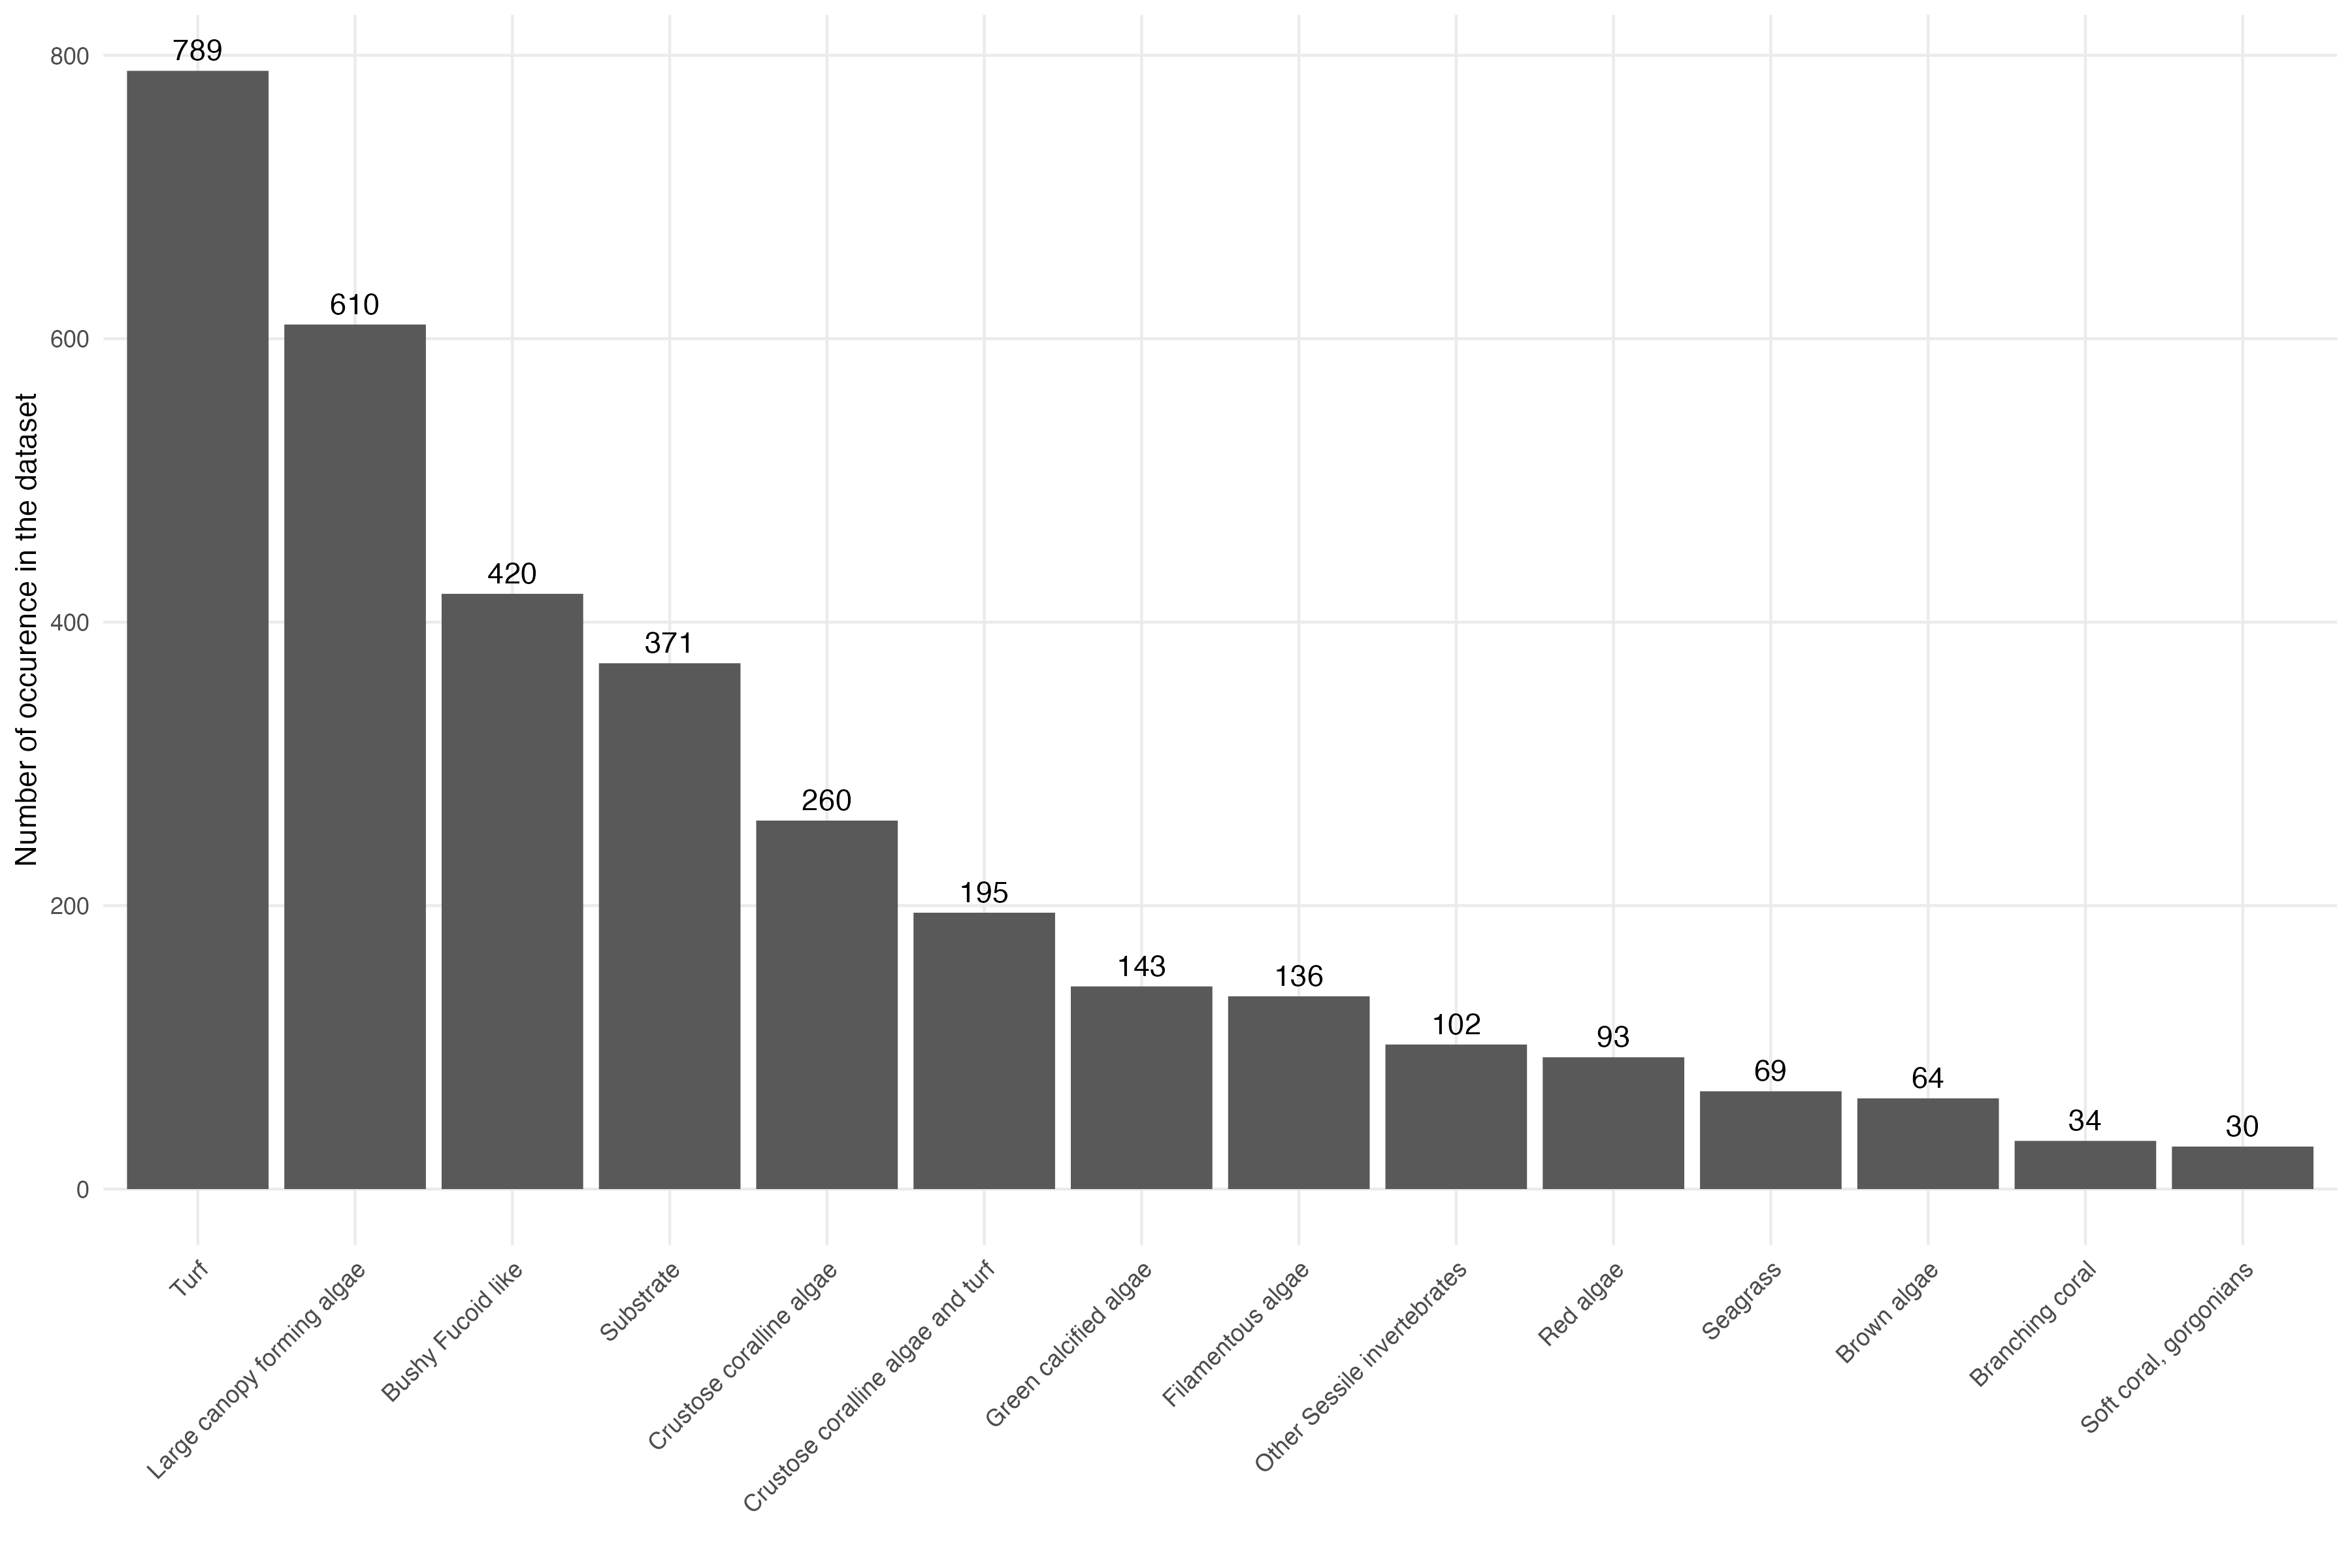
\includegraphics{03-Chapitre3/figures/supplementary/06-occurence_habitat_dataset.png}
\caption{Occurrence of the different habitat states in the
dataset}\label{fig:chap3figS1}
}
\end{figure}

\begin{figure}
\hypertarget{fig:chap3figS2}{%
\centering
\includegraphics{03-Chapitre3/figures/supplementary/05-pca_fishing.png}
\caption{PCA biplots of the fishing data.}\label{fig:chap3figS2}
}
\end{figure}

\begin{figure}
\hypertarget{fig:chap3figS3}{%
\centering
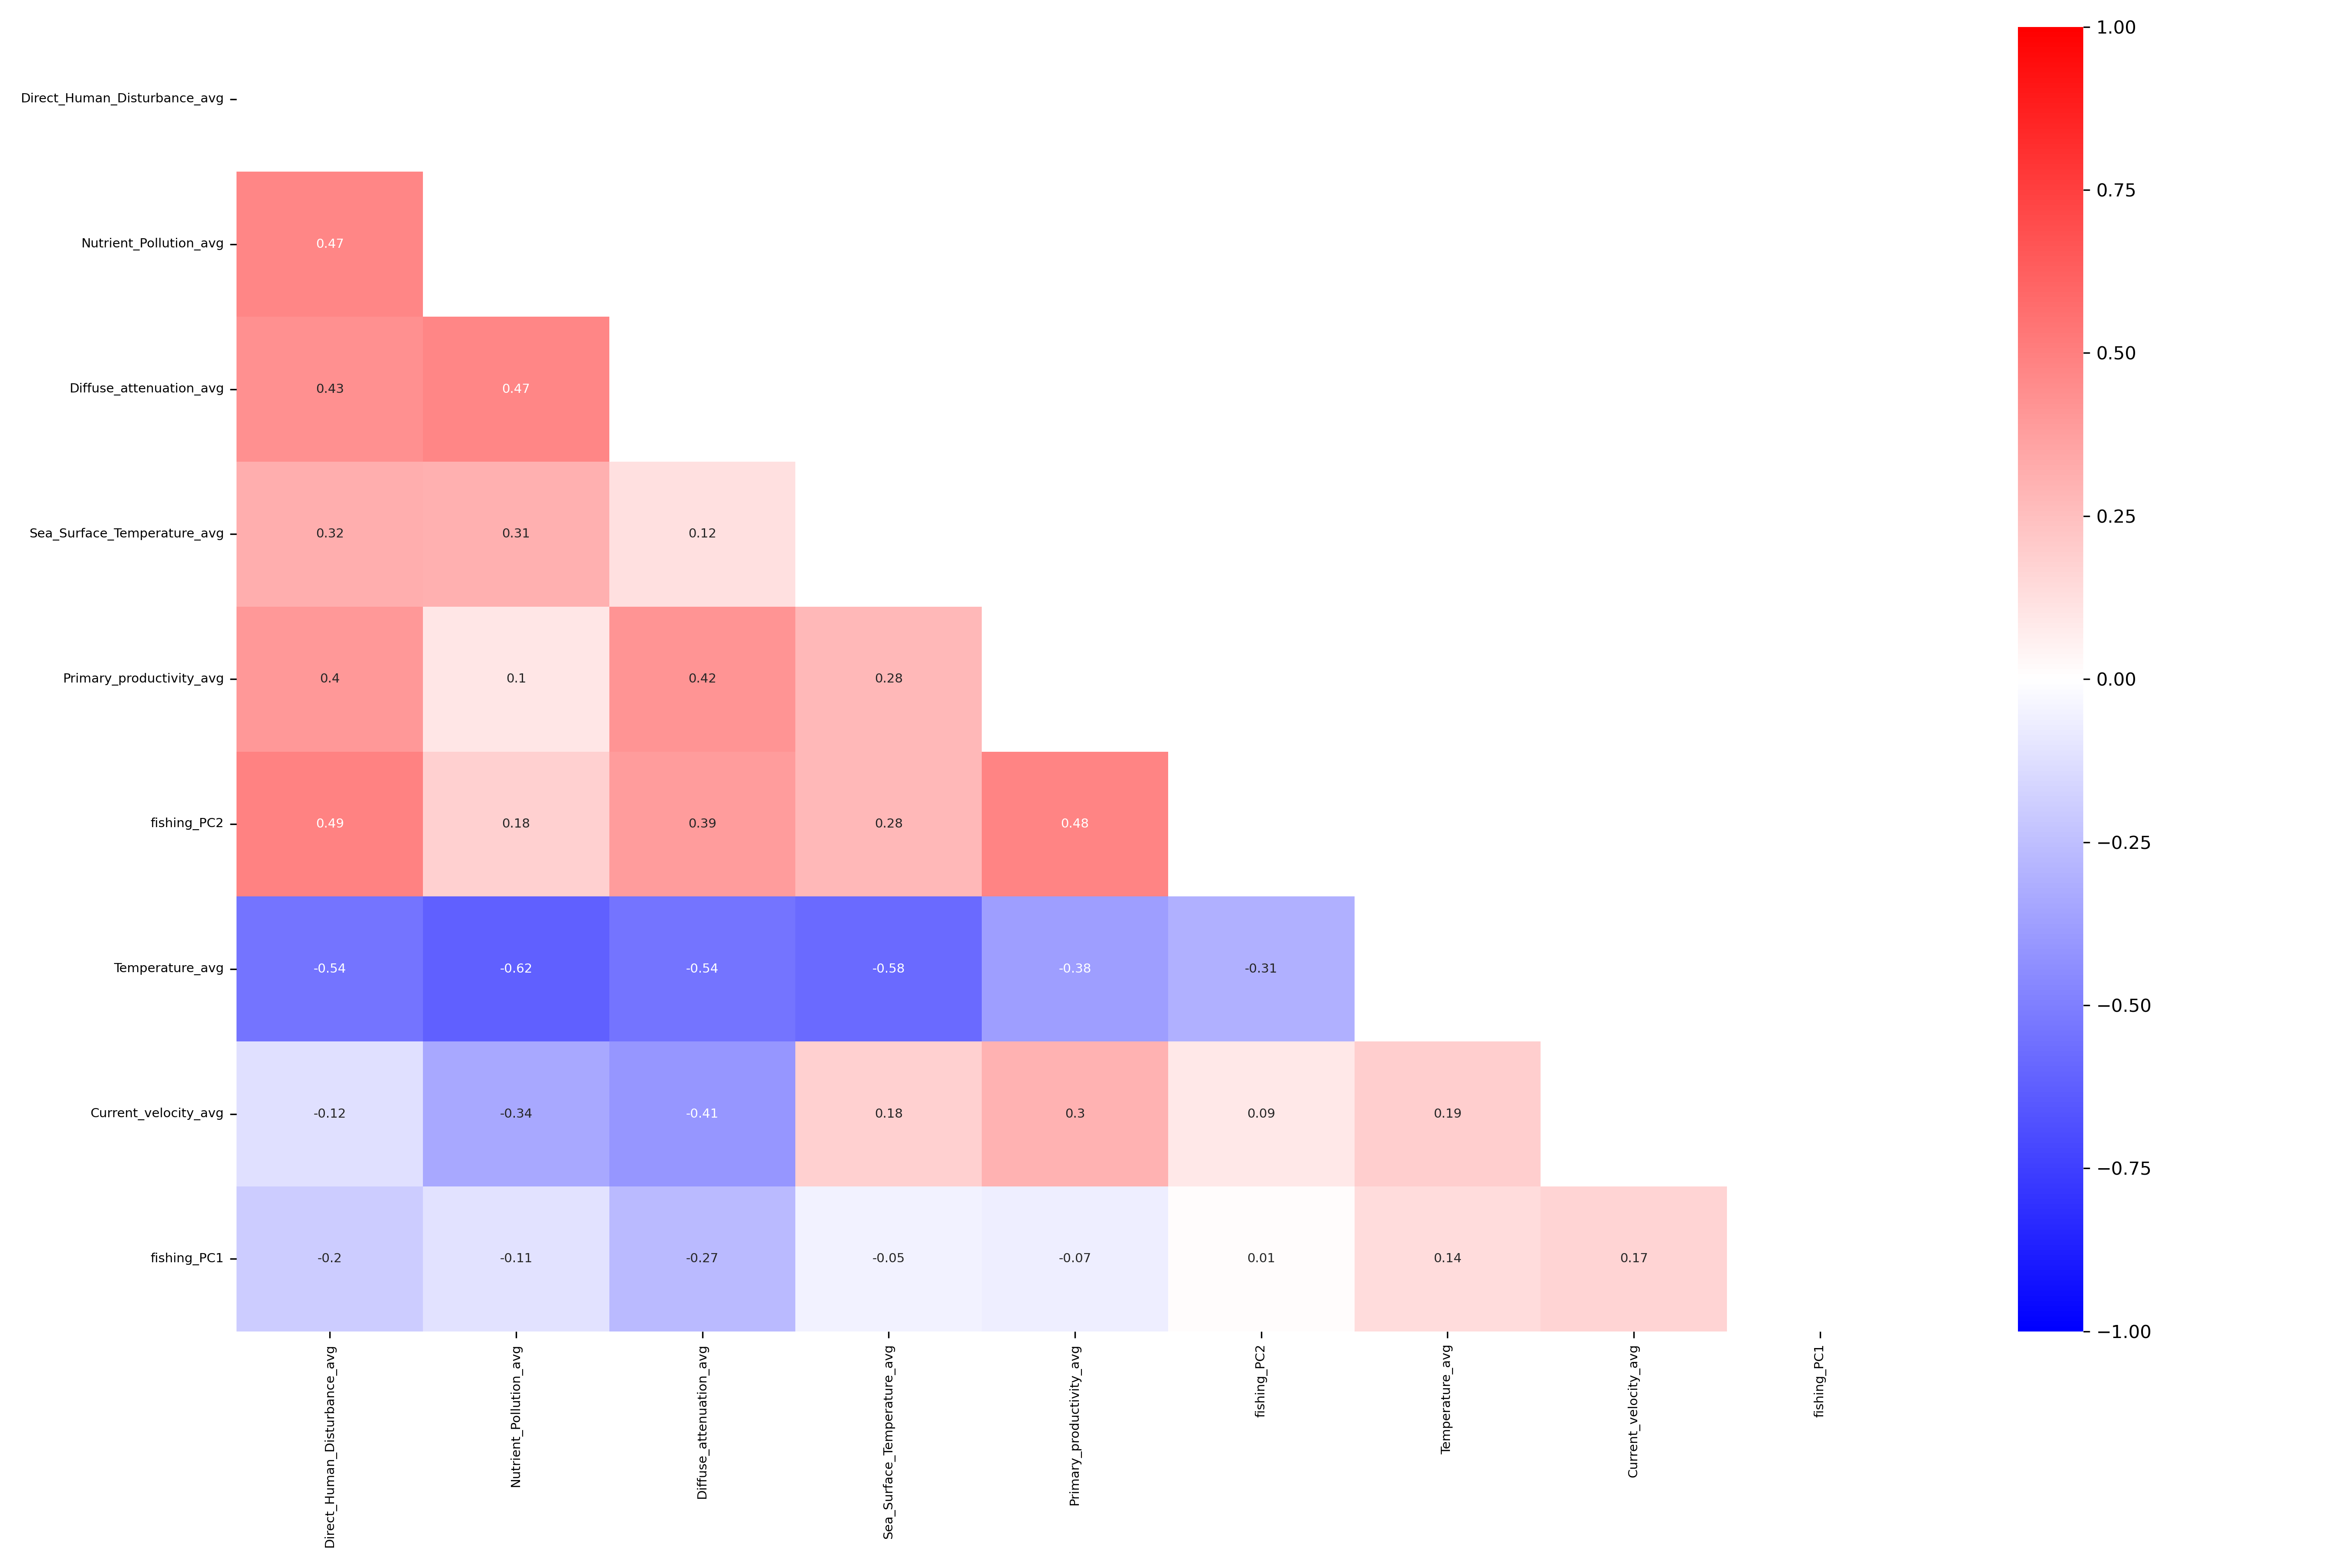
\includegraphics{03-Chapitre3/figures/supplementary/05c-corr_plot_all_vars.png}
\caption{Pearson's correlation matrix of selected
predictors.}\label{fig:chap3figS3}
}
\end{figure}

\begin{figure}
\hypertarget{fig:chap3figS4}{%
\centering
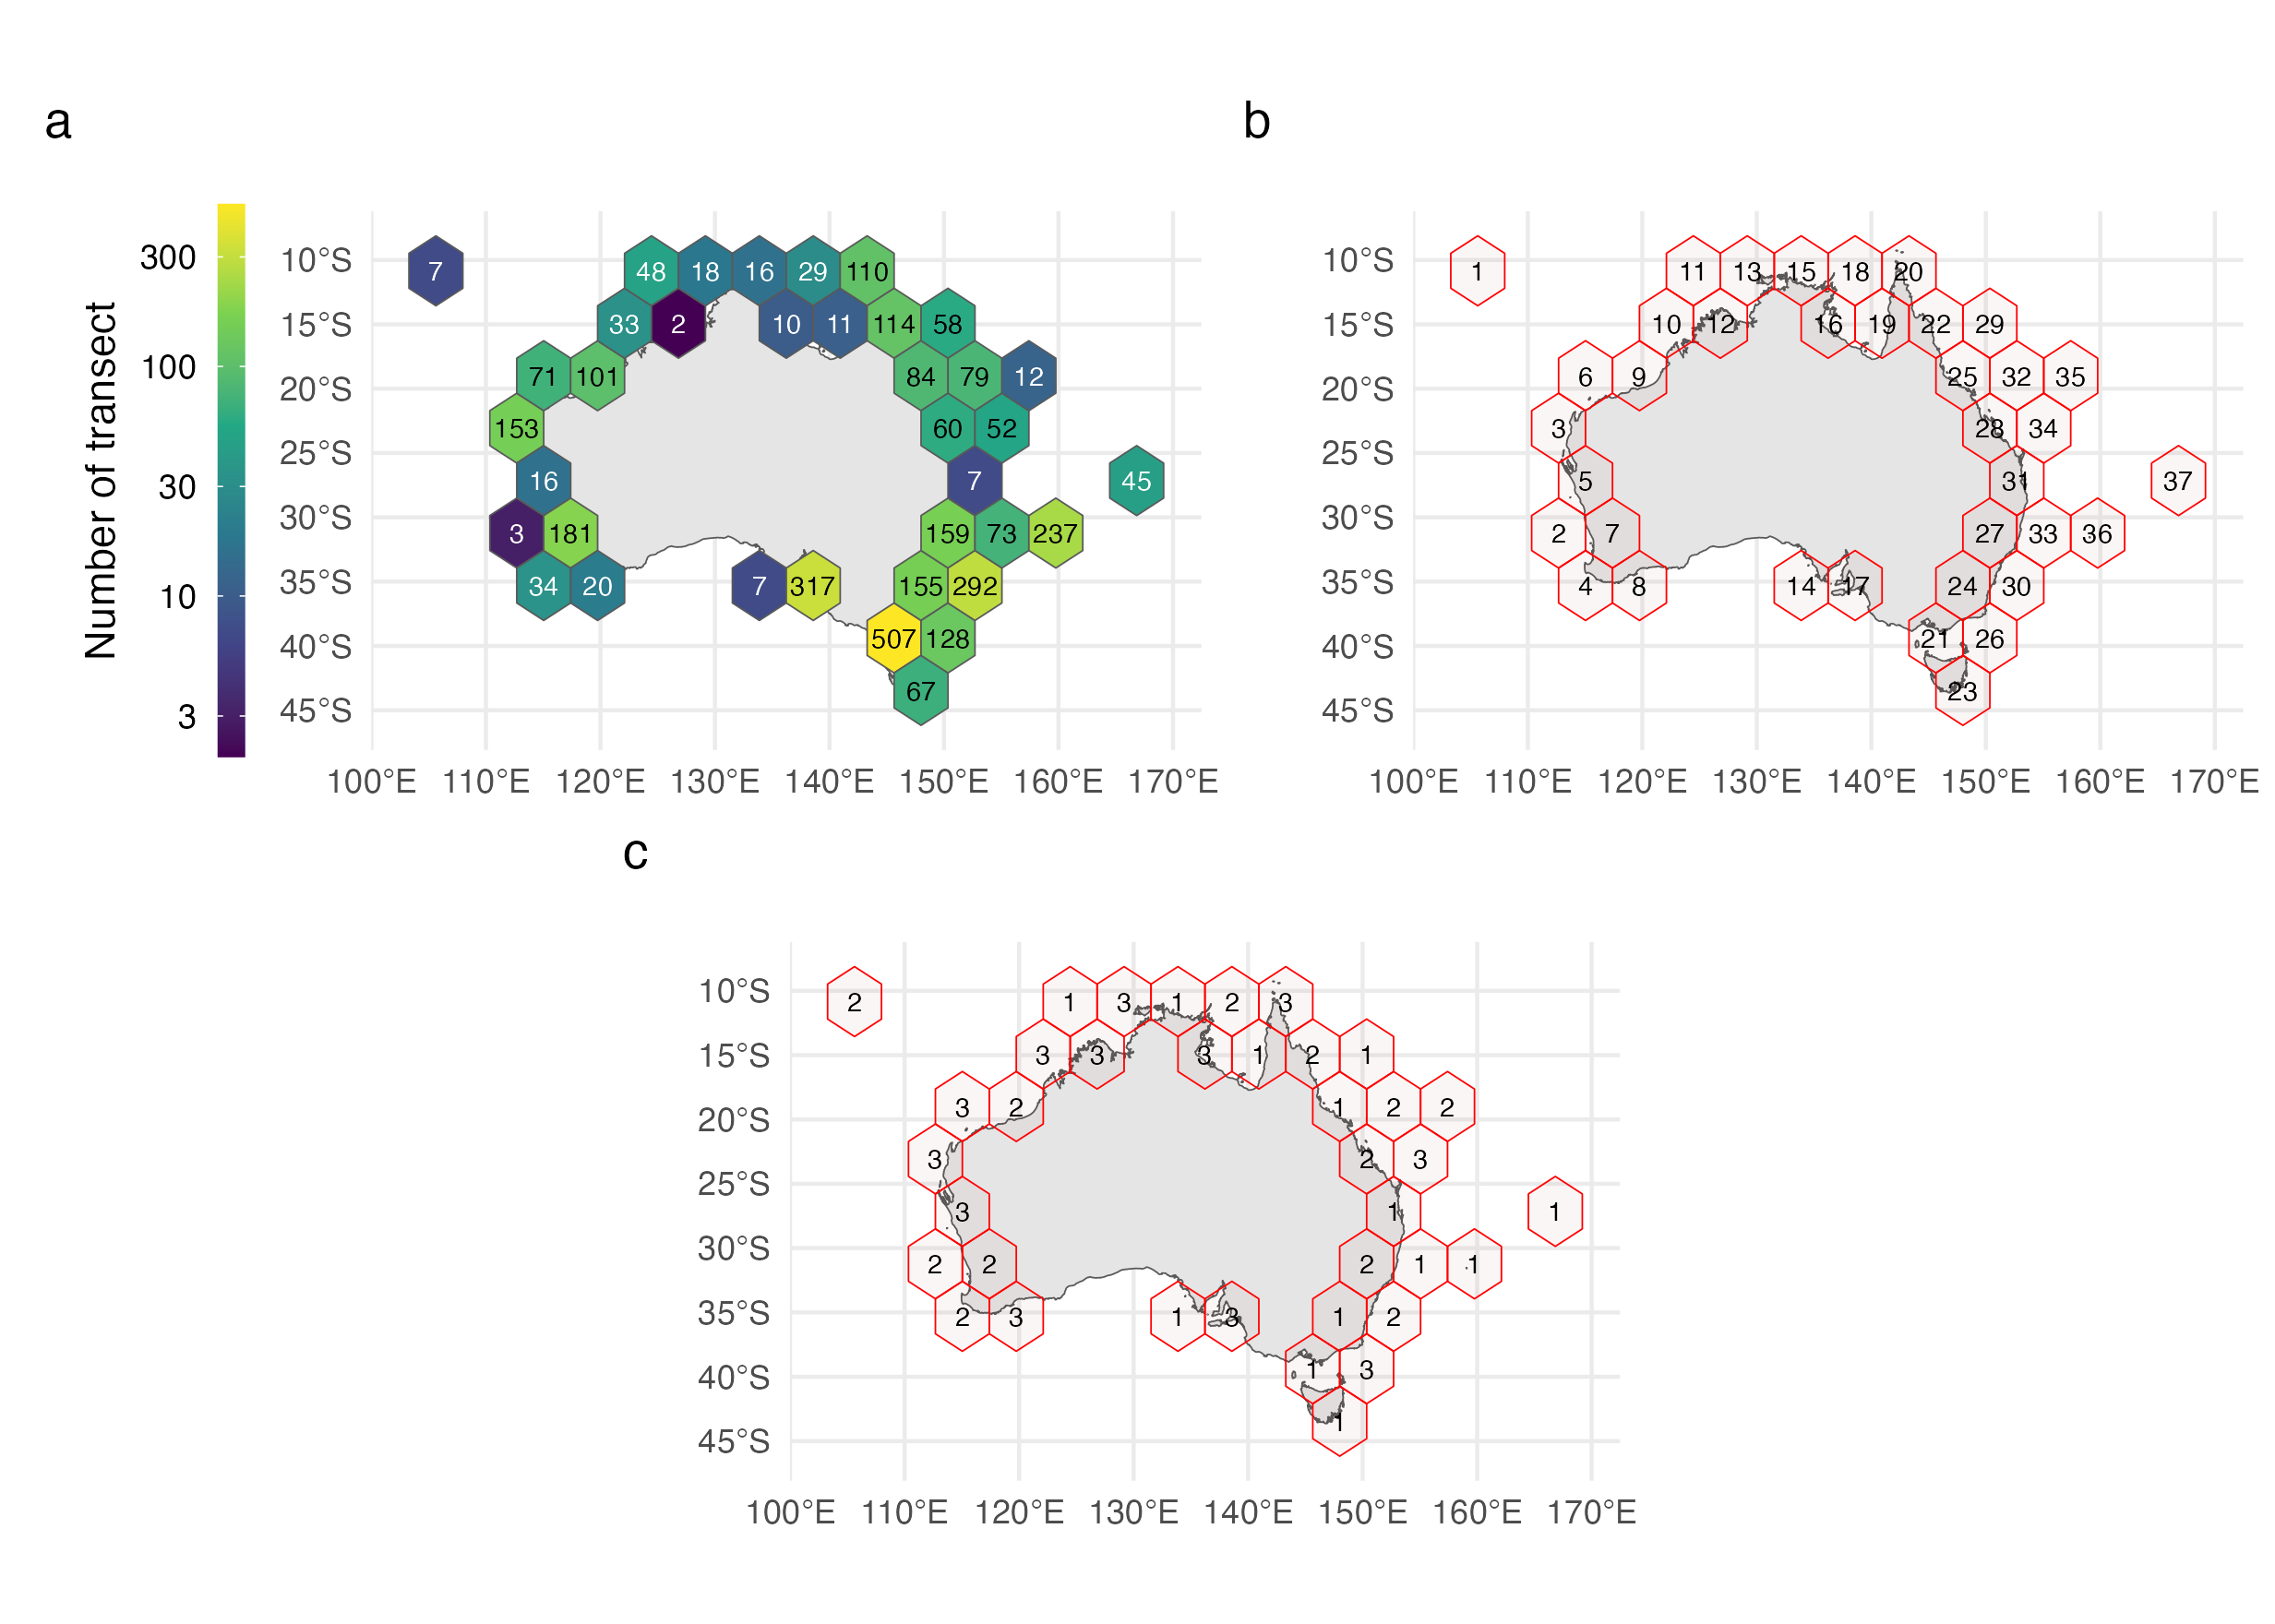
\includegraphics{03-Chapitre3/figures/supplementary/06-Spatial_fold_assignment.png}
\caption{a. Number of transect per spatial block. b. Map of the
distribution of spatial blocks along the Australian coast. c.~Map of
spatial block allocation in one of the three
folds.}\label{fig:chap3figS4}
}
\end{figure}

\begin{figure}
\hypertarget{fig:chap3figS5}{%
\centering
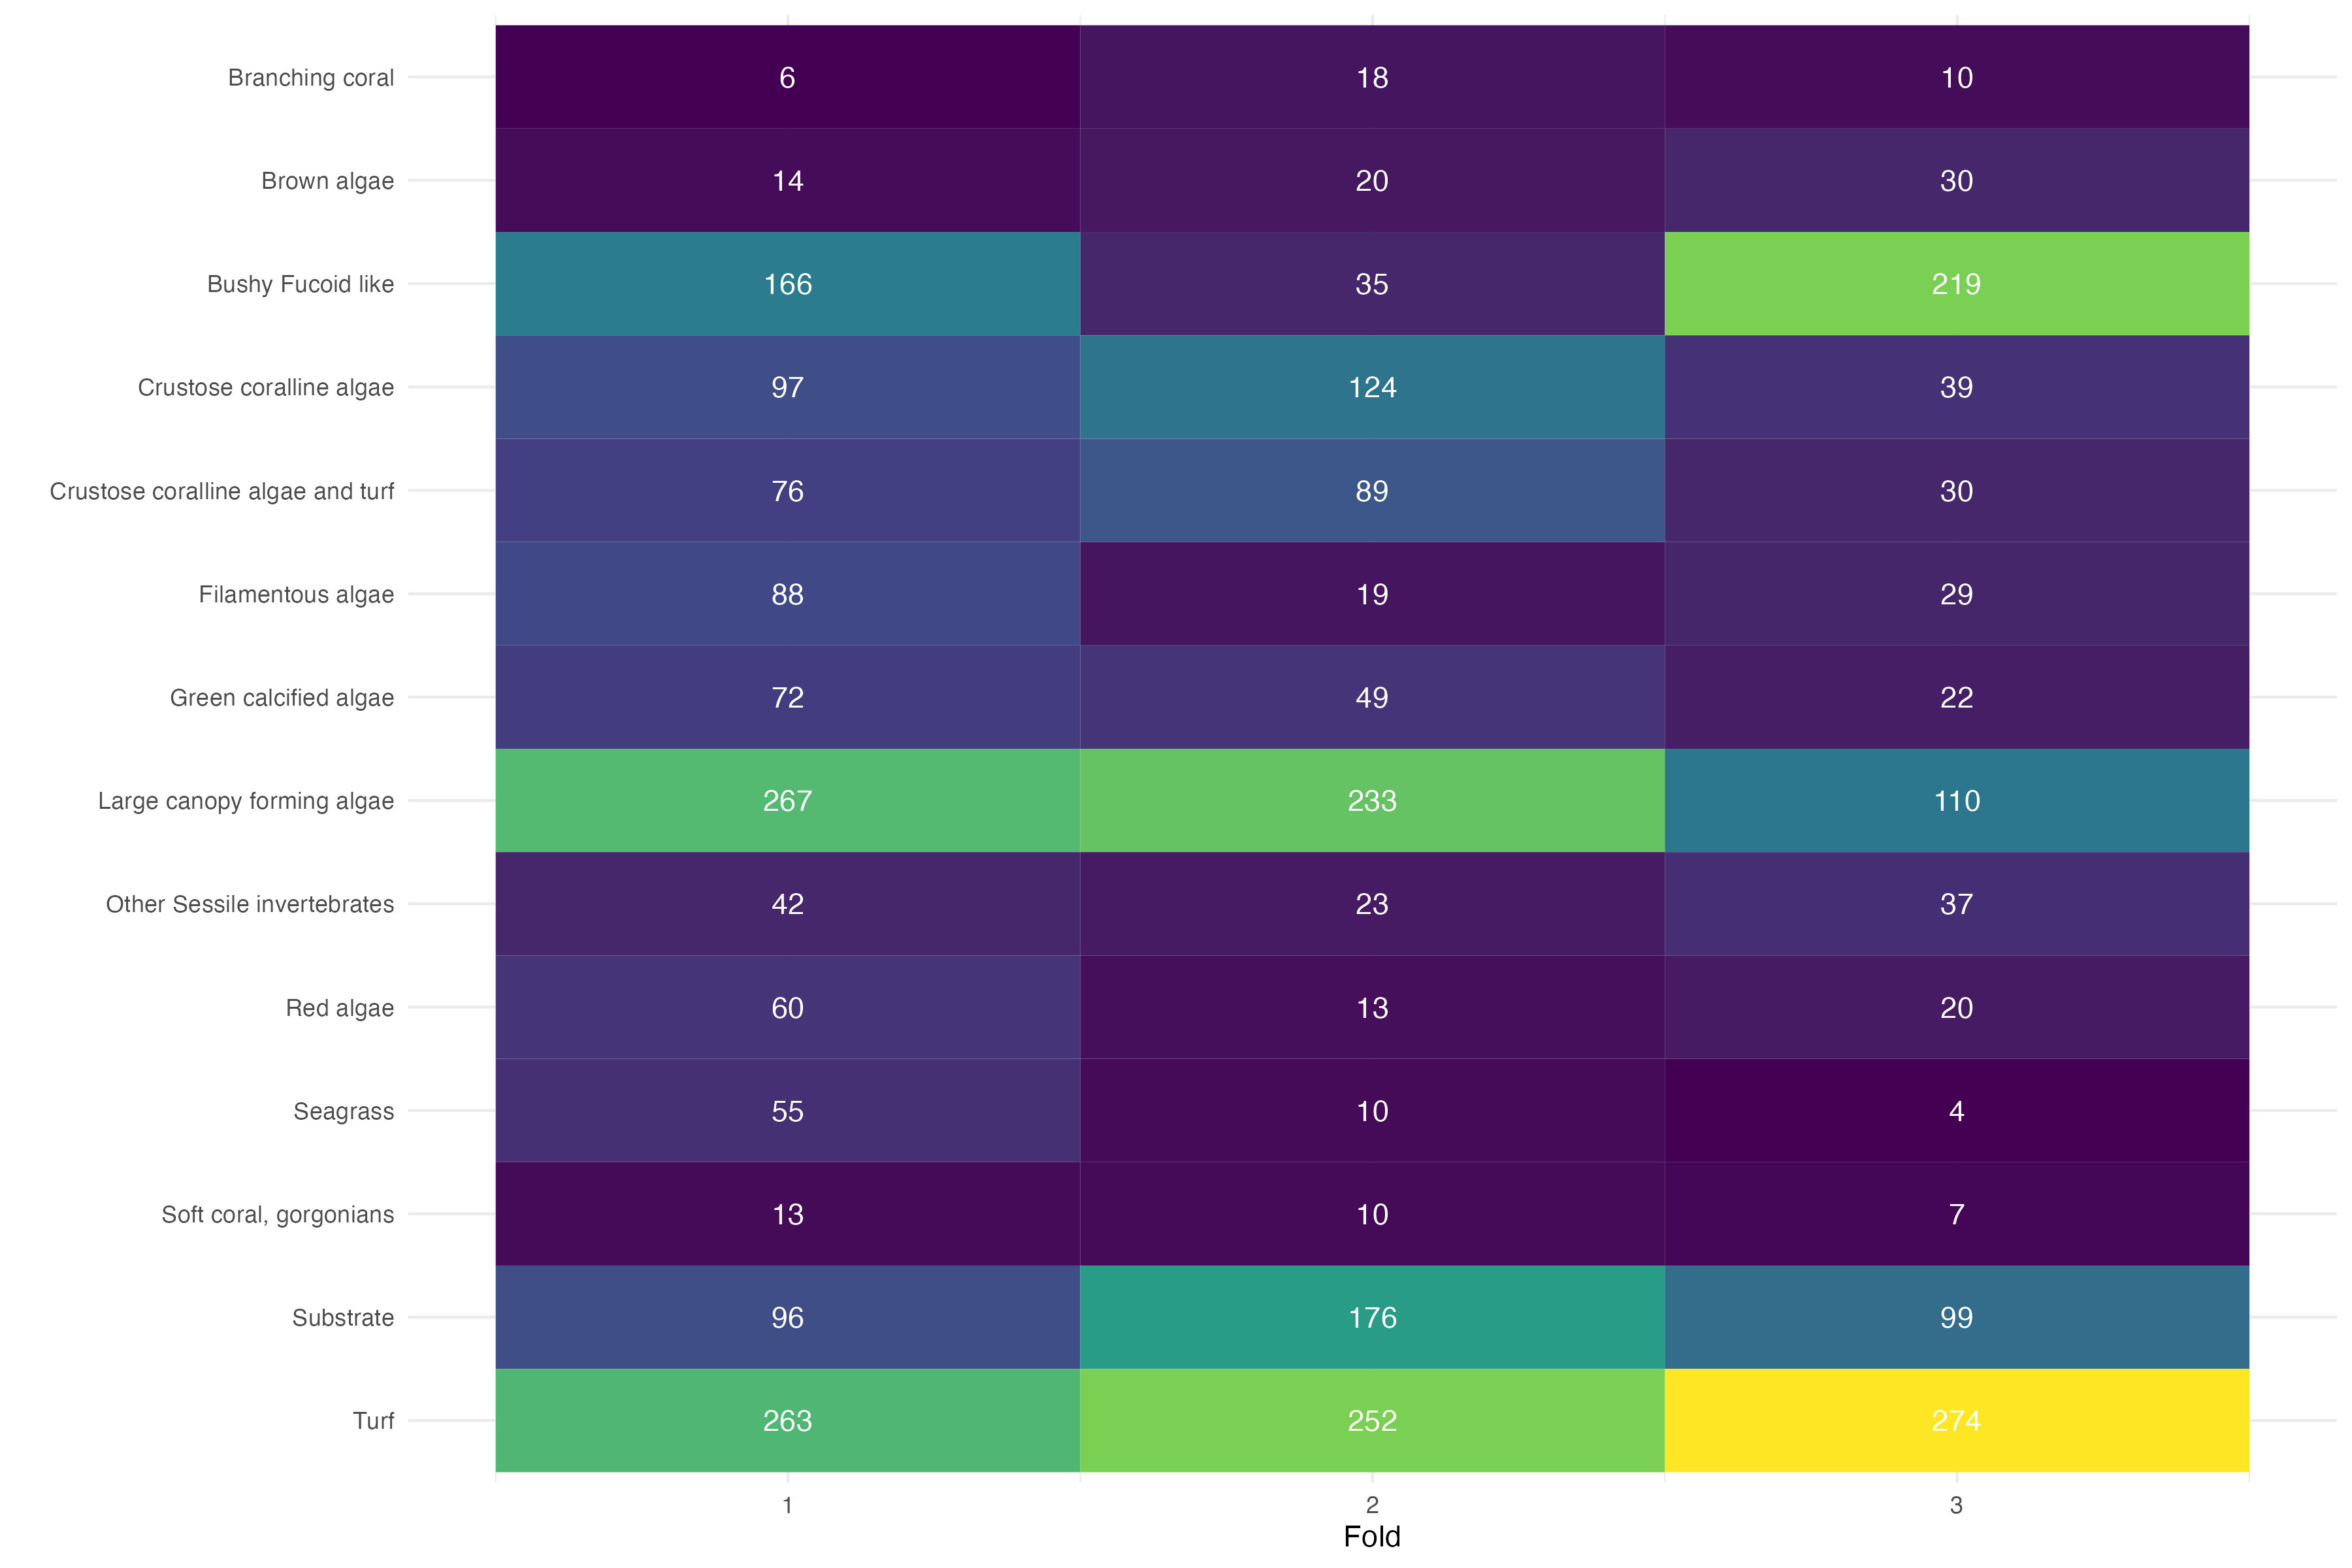
\includegraphics{03-Chapitre3/figures/supplementary/06-occurence_habitat_folds.png}
\caption{Number of occurrences of each habitat state per training and
test fold. The colour is based on the proportion represented by each
habitat state within the considered fold.}\label{fig:chap3figS5}
}
\end{figure}

\clearpage

\hypertarget{appendixB-chapter3}{%
\section*{Appendix B - Model fitting \&
Evaluation}\label{appendixB-chapter3}}
\addcontentsline{toc}{section}{Appendix B - Model fitting \& Evaluation}

\hypertarget{model-fit}{%
\subsection*{Model Fit}\label{model-fit}}

\hypertarget{hyperparameter-tunning}{%
\subsubsection*{Hyperparameter tunning}\label{hyperparameter-tunning}}

\hypertarget{tbl:chap3tblS2}{}
\begin{longtable}[]{@{}
  >{\raggedright\arraybackslash}p{(\columnwidth - 4\tabcolsep) * \real{0.1263}}
  >{\raggedright\arraybackslash}p{(\columnwidth - 4\tabcolsep) * \real{0.6768}}
  >{\raggedright\arraybackslash}p{(\columnwidth - 4\tabcolsep) * \real{0.1970}}@{}}
\caption{\label{tbl:chap3tblS2}Description of the hyperparameters tuned
and their values according to the \emph{scikit-learn}
documentation.}\tabularnewline
\toprule\noalign{}
\begin{minipage}[b]{\linewidth}\raggedright
\textbf{Hyperparameter name}
\end{minipage} & \begin{minipage}[b]{\linewidth}\raggedright
\textbf{Description}
\end{minipage} & \begin{minipage}[b]{\linewidth}\raggedright
\textbf{Values}
\end{minipage} \\
\midrule\noalign{}
\endfirsthead
\toprule\noalign{}
\begin{minipage}[b]{\linewidth}\raggedright
\textbf{Hyperparameter name}
\end{minipage} & \begin{minipage}[b]{\linewidth}\raggedright
\textbf{Description}
\end{minipage} & \begin{minipage}[b]{\linewidth}\raggedright
\textbf{Values}
\end{minipage} \\
\midrule\noalign{}
\endhead
\bottomrule\noalign{}
\endlastfoot
\emph{n\_estimators} & The number of trees in the forest. &
\(\{100, 200, 300, \ldots, 3000\}\) \\
\emph{max\_features} & The number of predictors to consider when looking
for the best split. & \(\{2, 3, 4, \ldots, 8\}\) \\
\emph{max\_depth} & The maximum depth of each tree. If \(\infty\), then
nodes are expanded until all leaves are pure or contain less than 2
samples & \(\{5, 10, 15, \ldots, 100, \infty\}\) \\
\end{longtable}

\hypertarget{confusion-matrix}{%
\subsubsection*{Confusion Matrix}\label{confusion-matrix}}

\begin{figure}
\hypertarget{fig:chap3figS6}{%
\centering
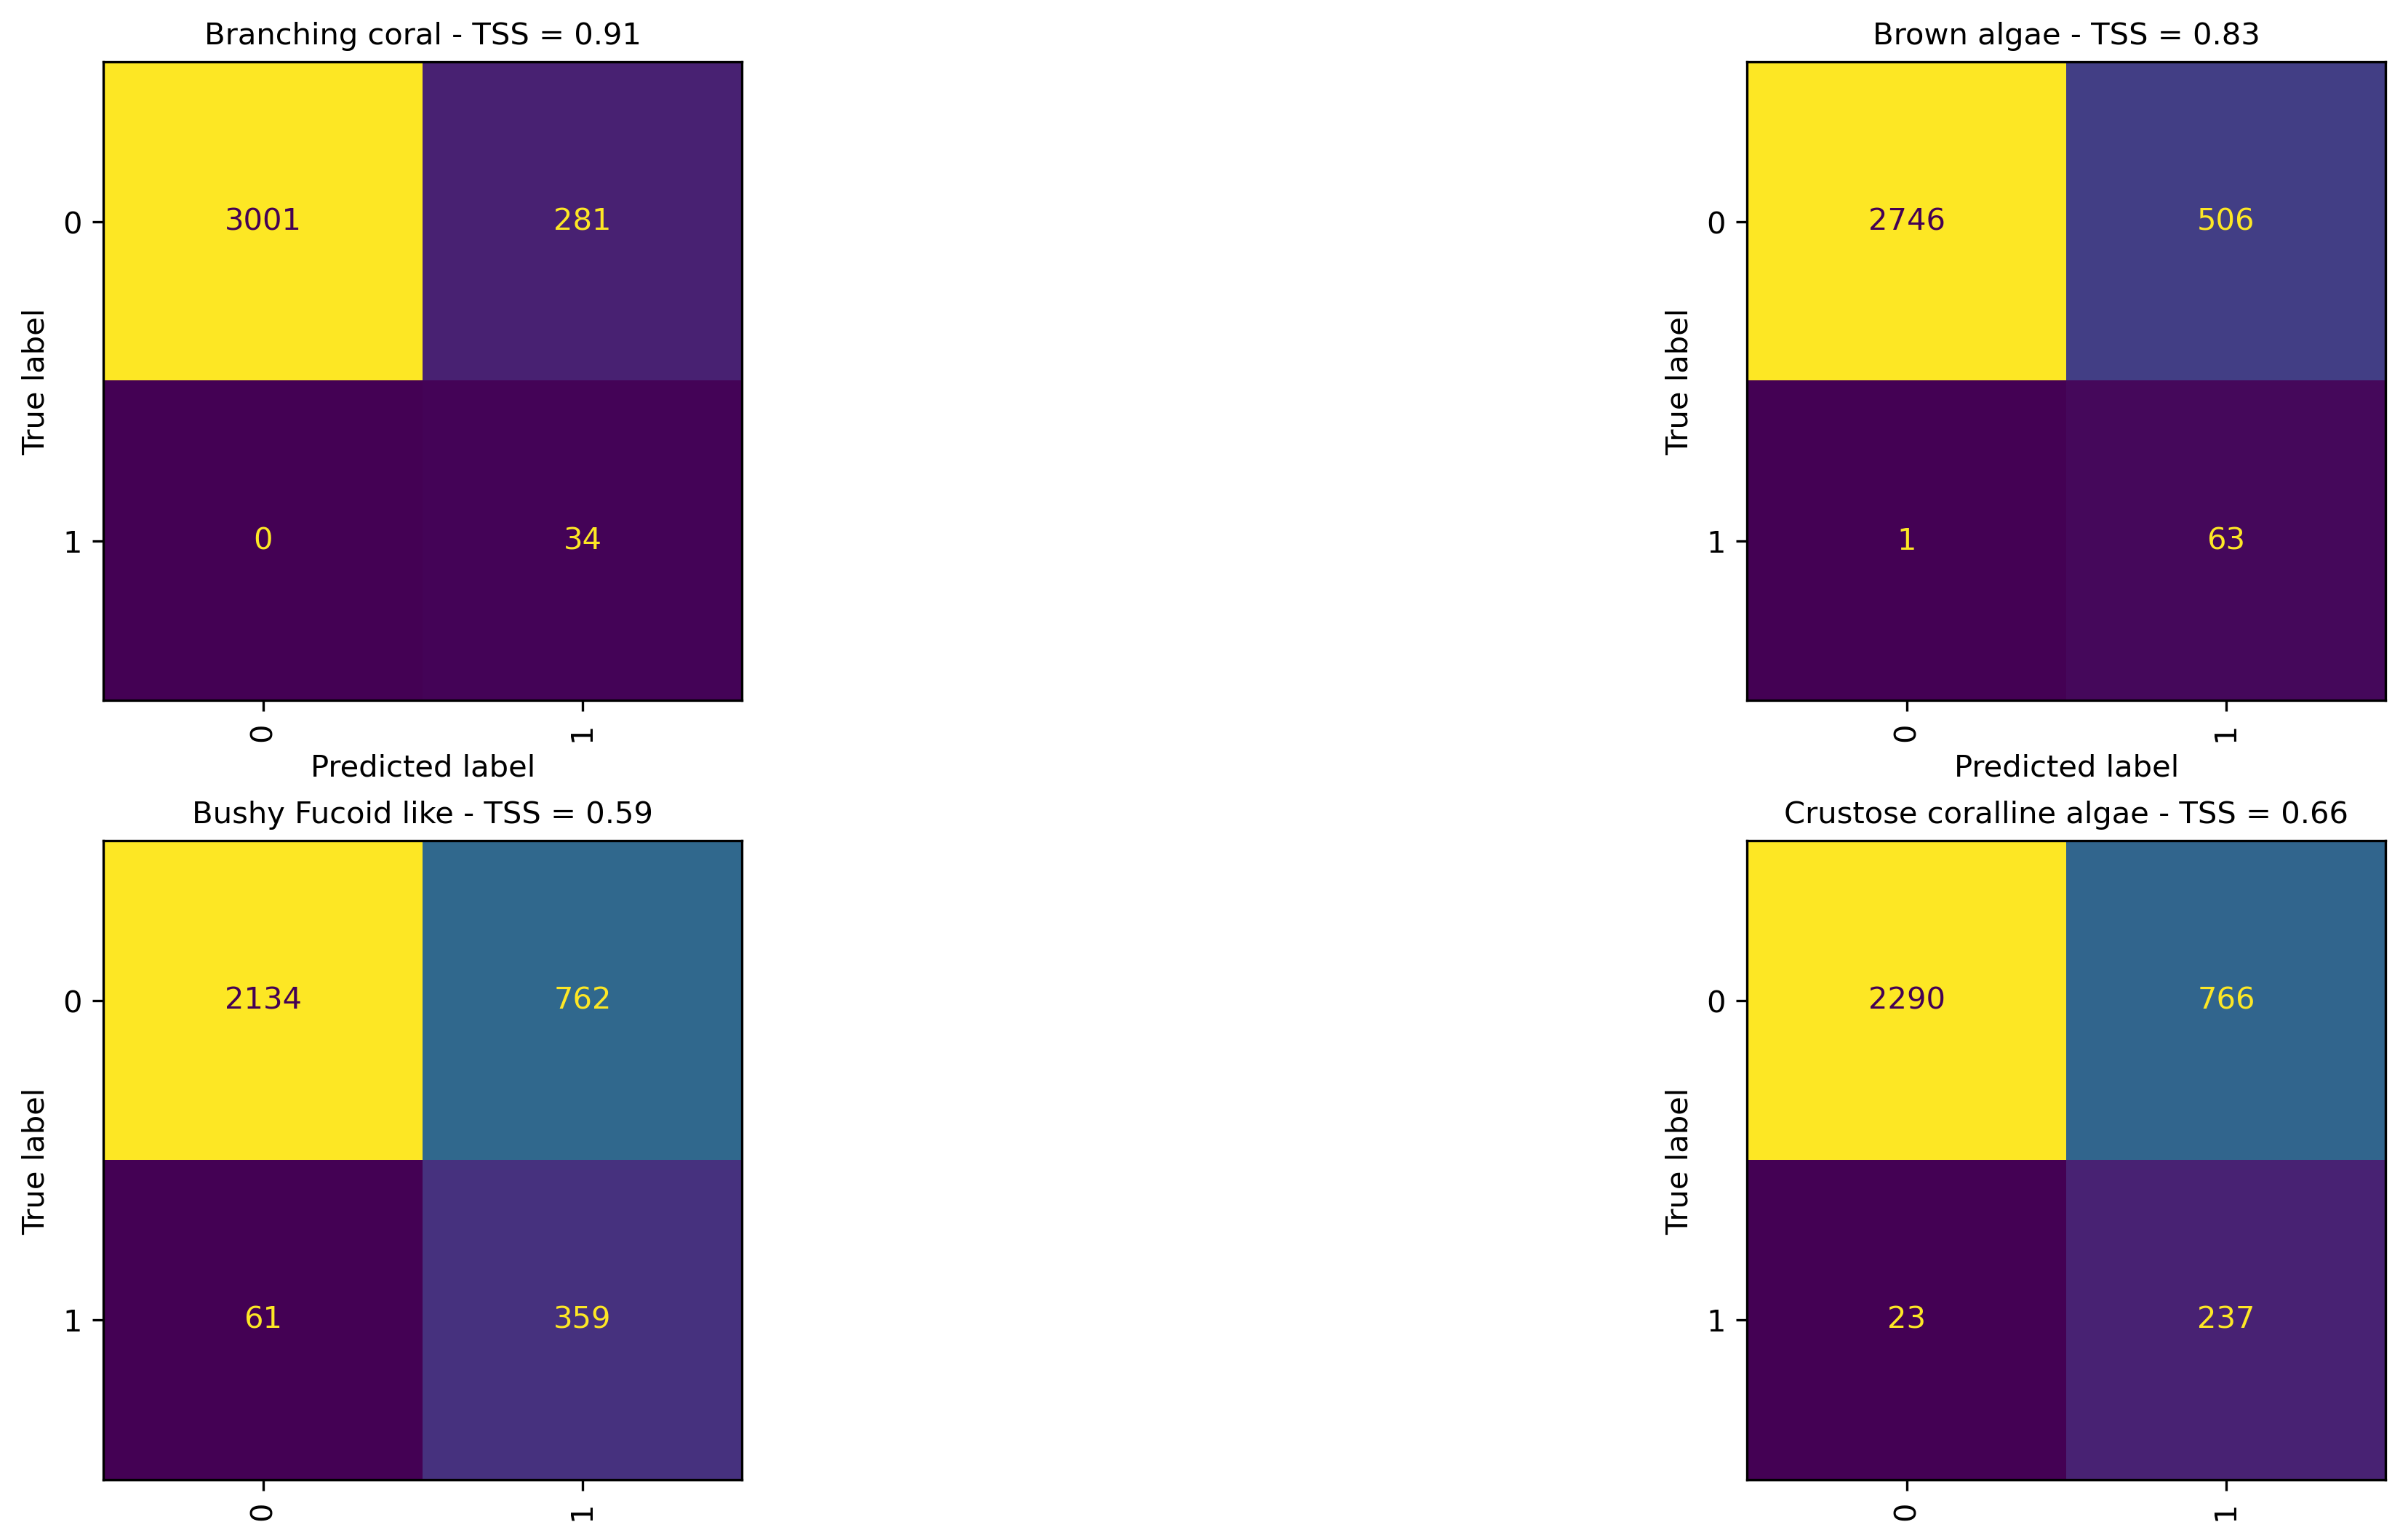
\includegraphics{03-Chapitre3/figures/supplementary/03-confusion_matrix_train_all_a.png}
\caption{Confusion Matrix of the explanatory
power.}\label{fig:chap3figS6}
}
\end{figure}
\begin{figure}
\ContinuedFloat
\centering
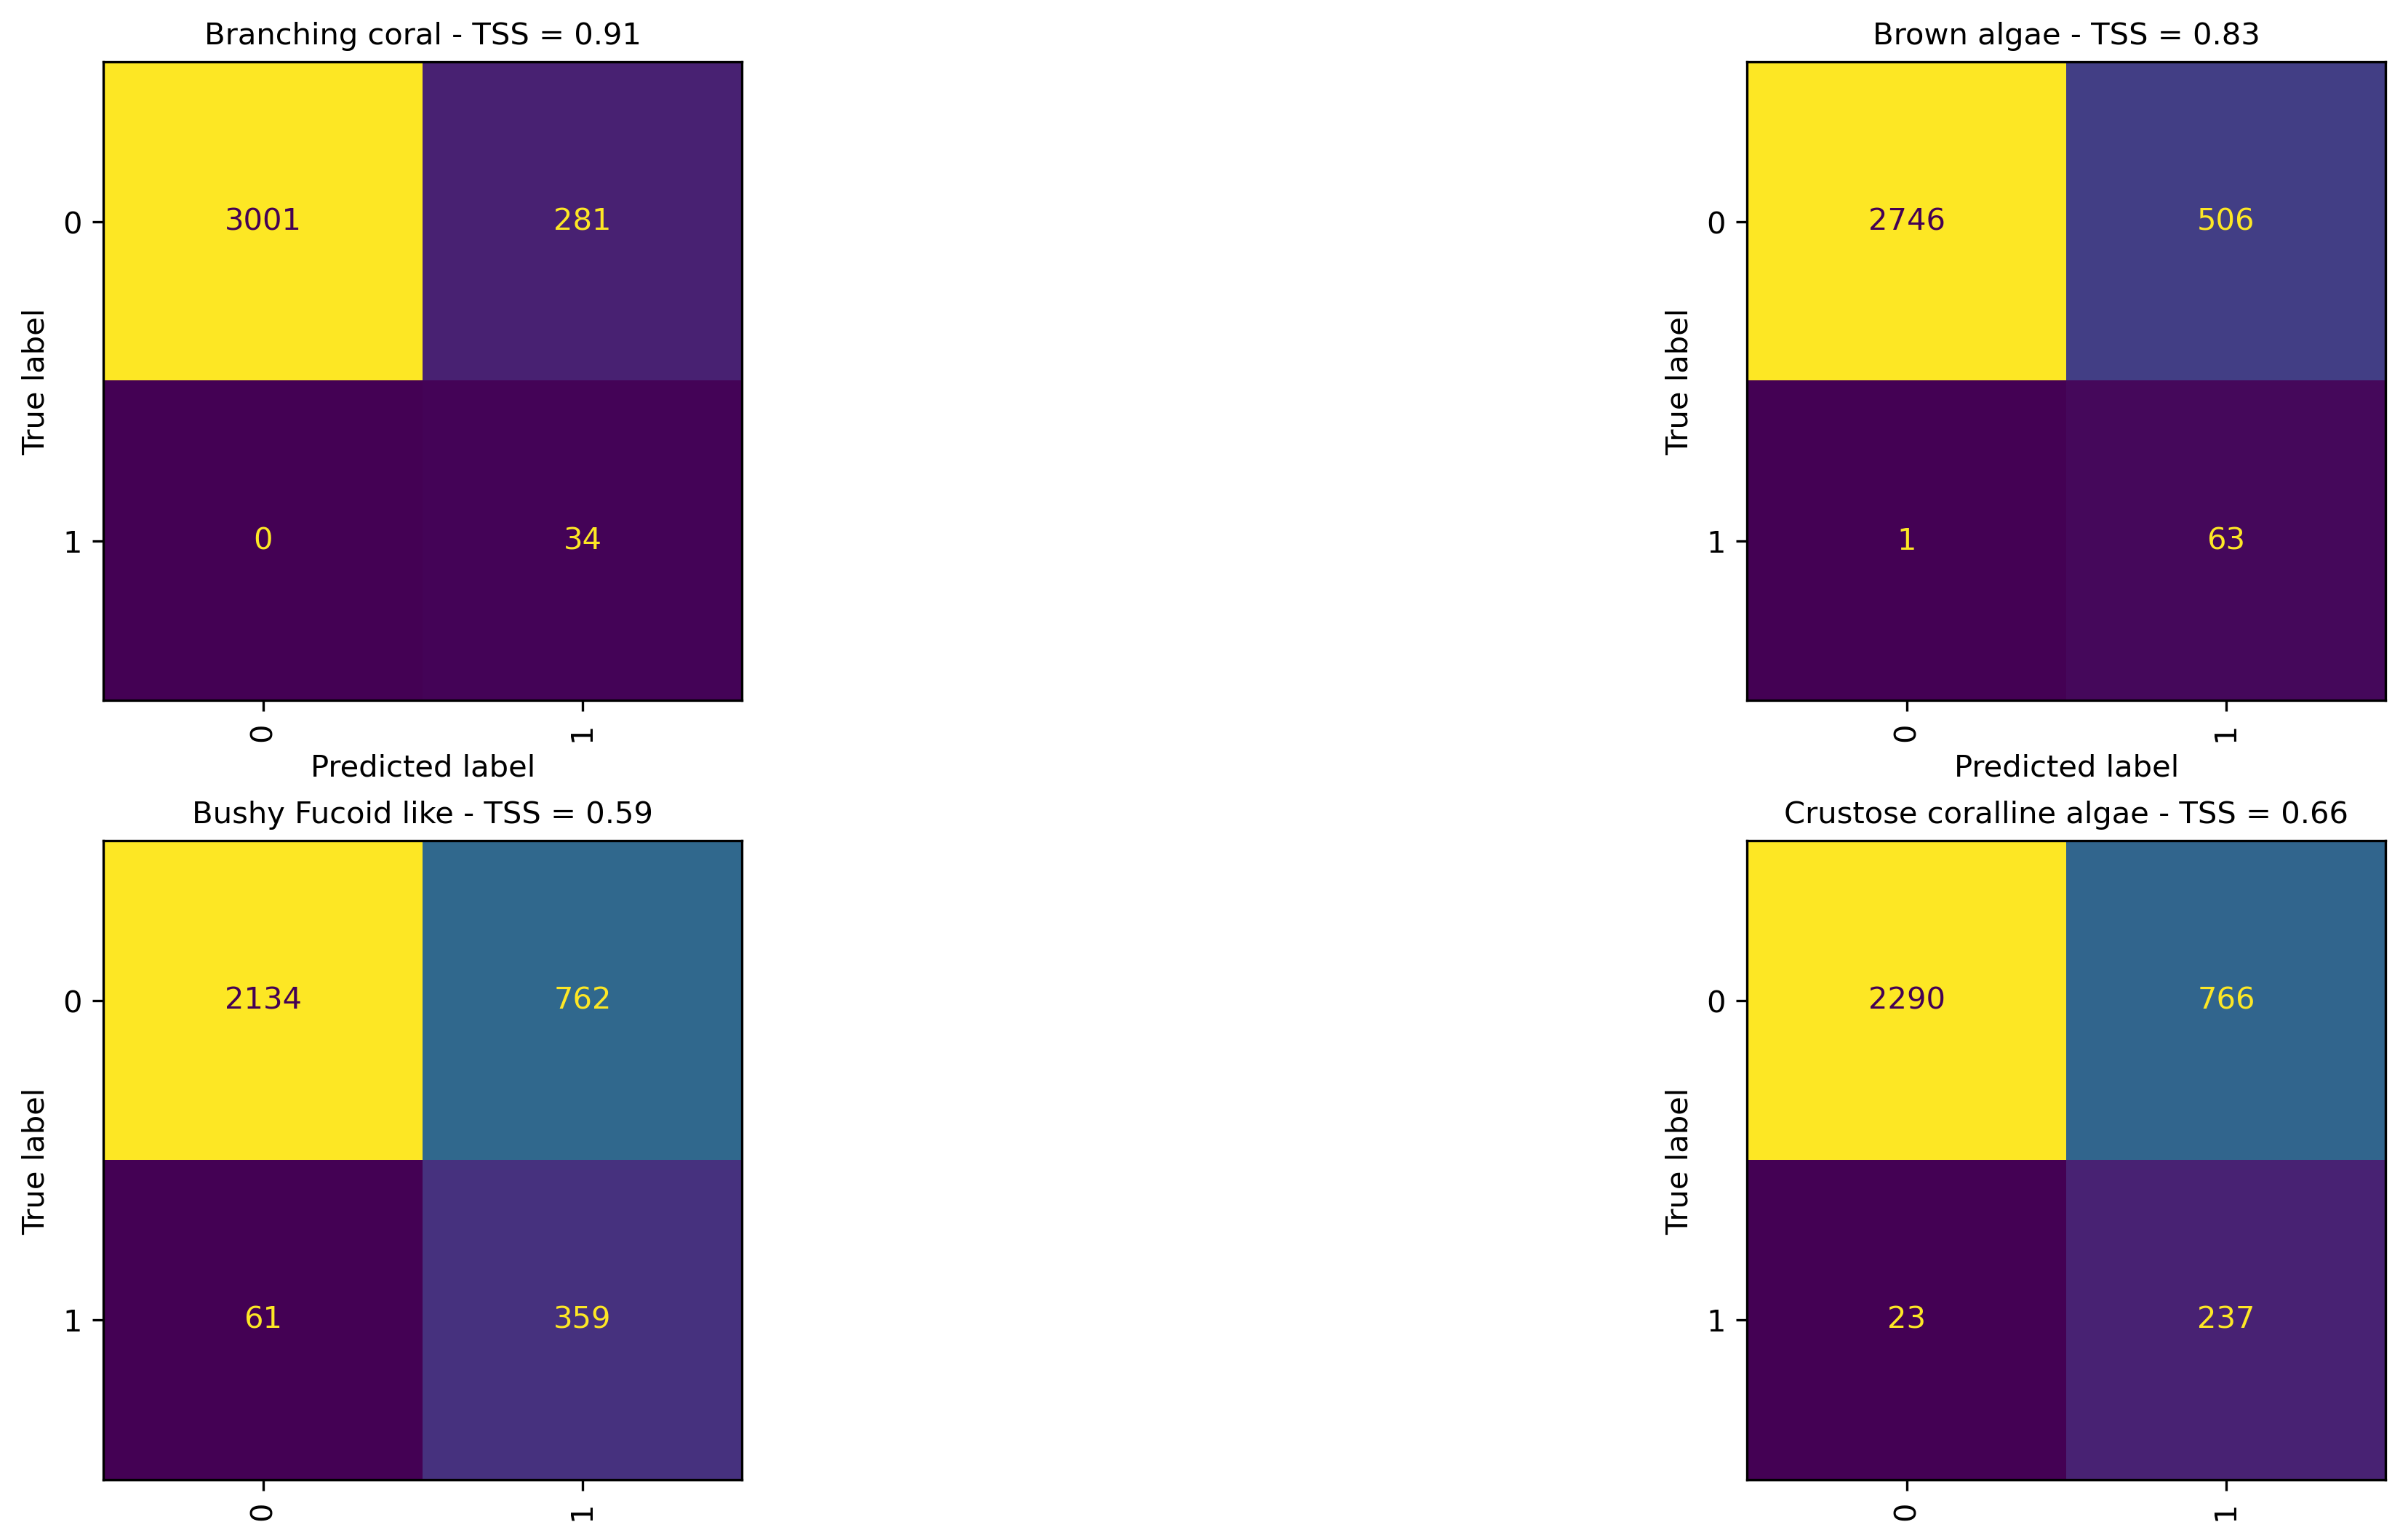
\includegraphics{03-Chapitre3/figures/supplementary/03-confusion_matrix_train_all_b.png}
\caption{Confusion Matrix of the explanatory
power.}
\end{figure}
\begin{figure}
\ContinuedFloat
\centering
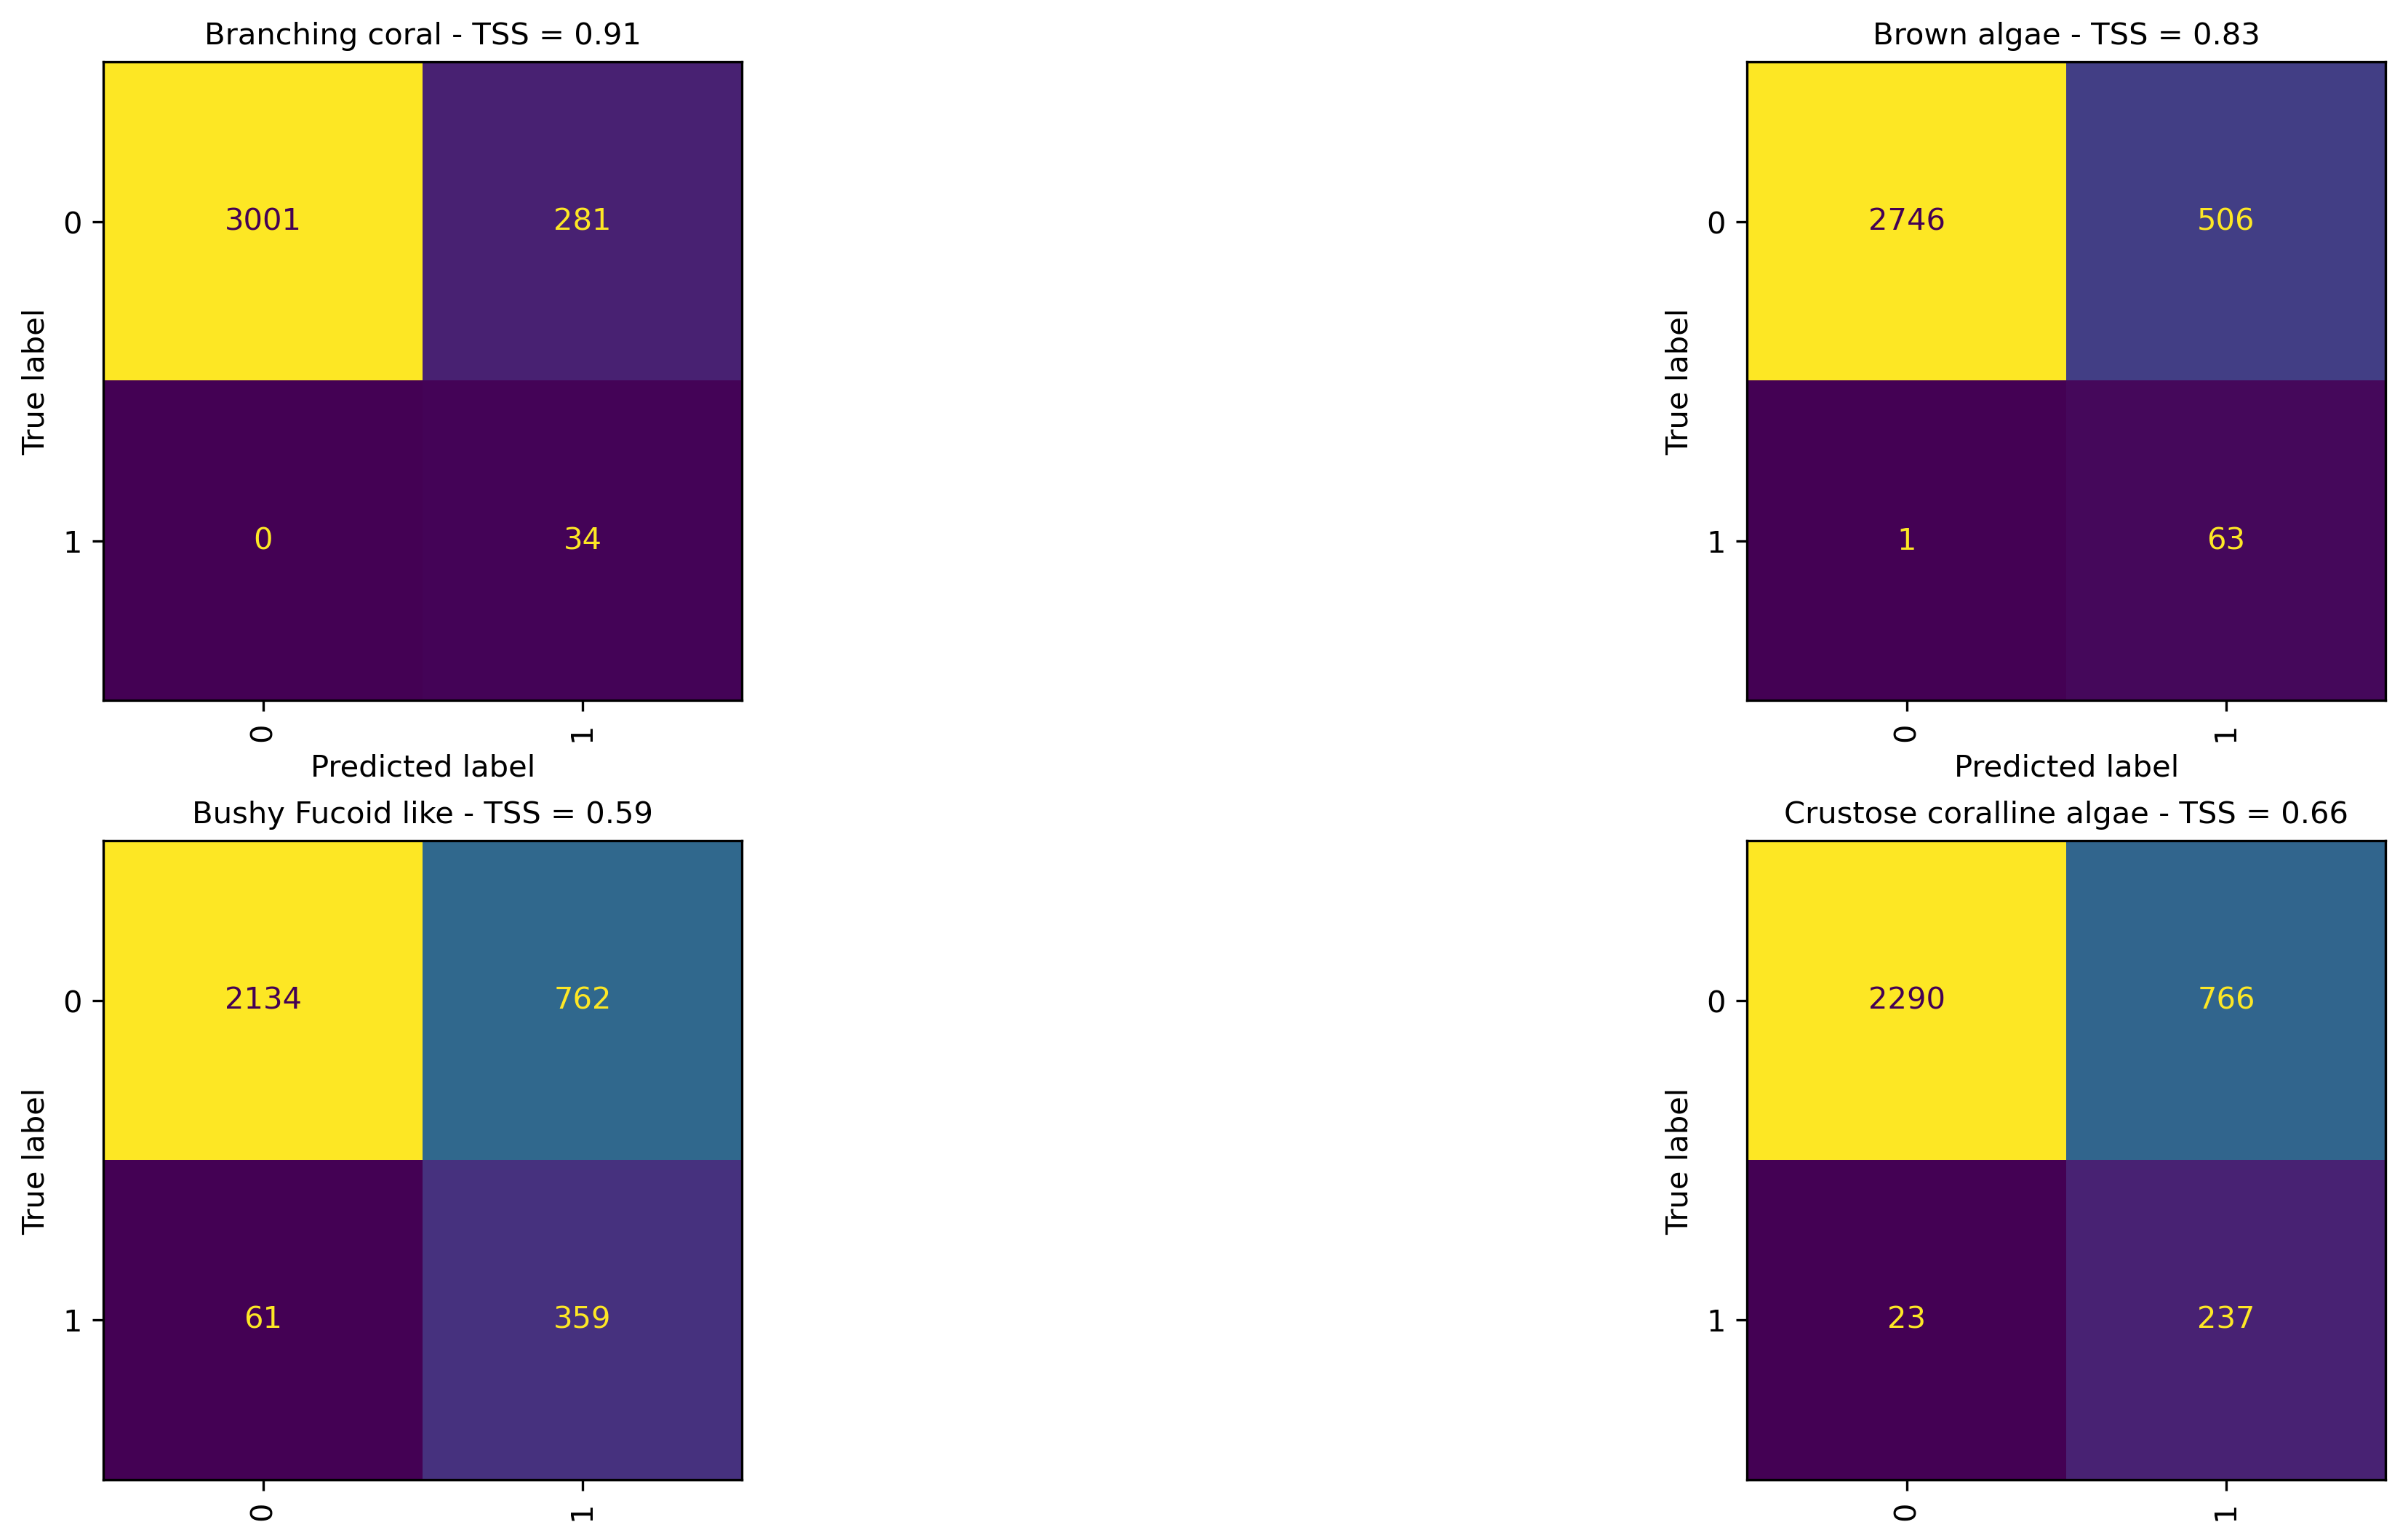
\includegraphics{03-Chapitre3/figures/supplementary/03-confusion_matrix_train_all_c.png}
\caption{Confusion Matrix of the explanatory
power.}
\end{figure}
\begin{figure}
\ContinuedFloat
\centering
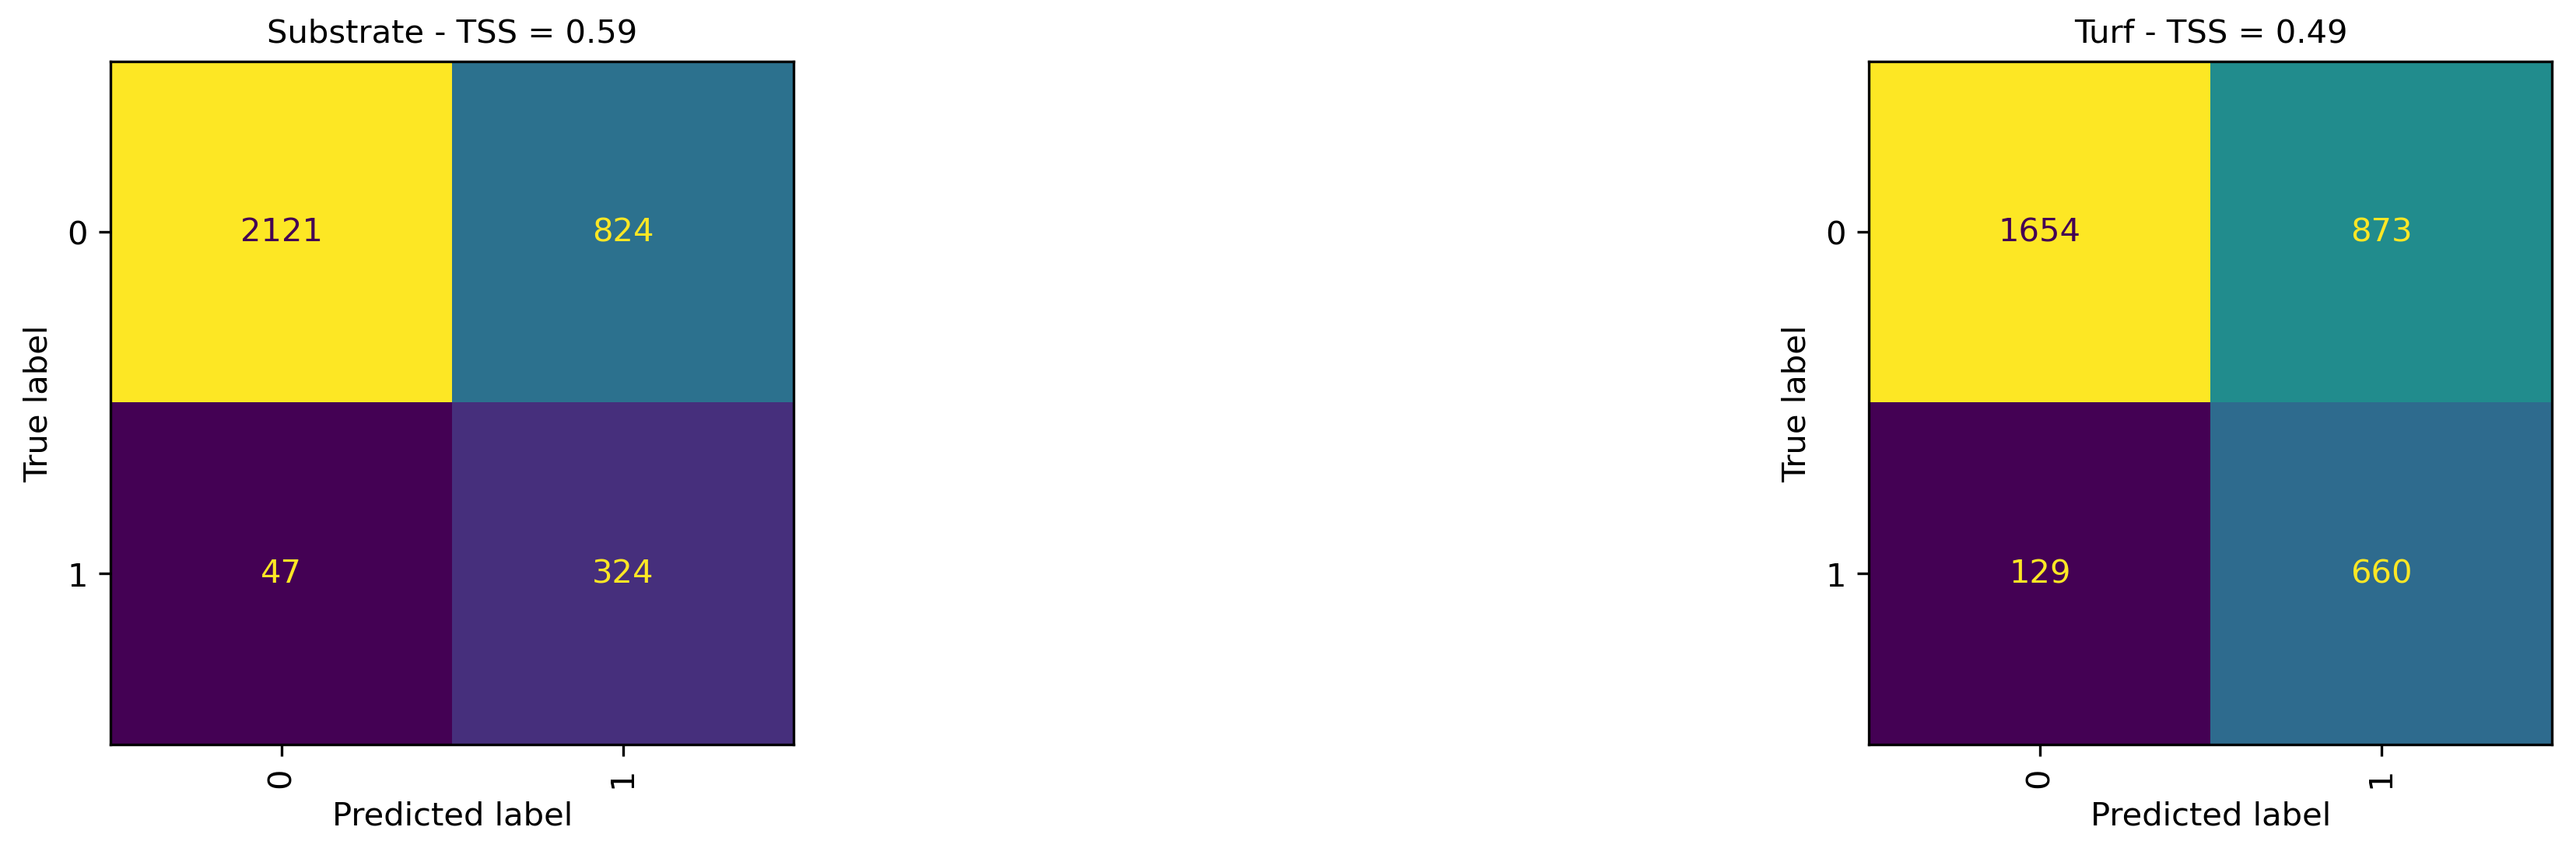
\includegraphics{03-Chapitre3/figures/supplementary/03-confusion_matrix_train_all_d.png}
\caption{Confusion Matrix of the explanatory
power.}
\end{figure}


\hypertarget{probability-distribution-of-habitat-states}{%
\subsubsection*{Probability distribution of habitat
states}\label{probability-distribution-of-habitat-states}}

\begin{figure}
\hypertarget{fig:chap3figS7}{%
\centering
\includegraphics{03-Chapitre3/figures/supplementary/03-hab_probability.png}
\caption{Distribution of occurrence probabilities for each habitat
state. The dotted line represents the threshold optimised by MaxTSS to
binarise the predictions.}\label{fig:chap3figS7}
}
\end{figure}

\hypertarget{auc-curves}{%
\subsubsection*{AUC Curves}\label{auc-curves}}

\begin{figure}
\hypertarget{fig:chap3figS8}{%
\centering
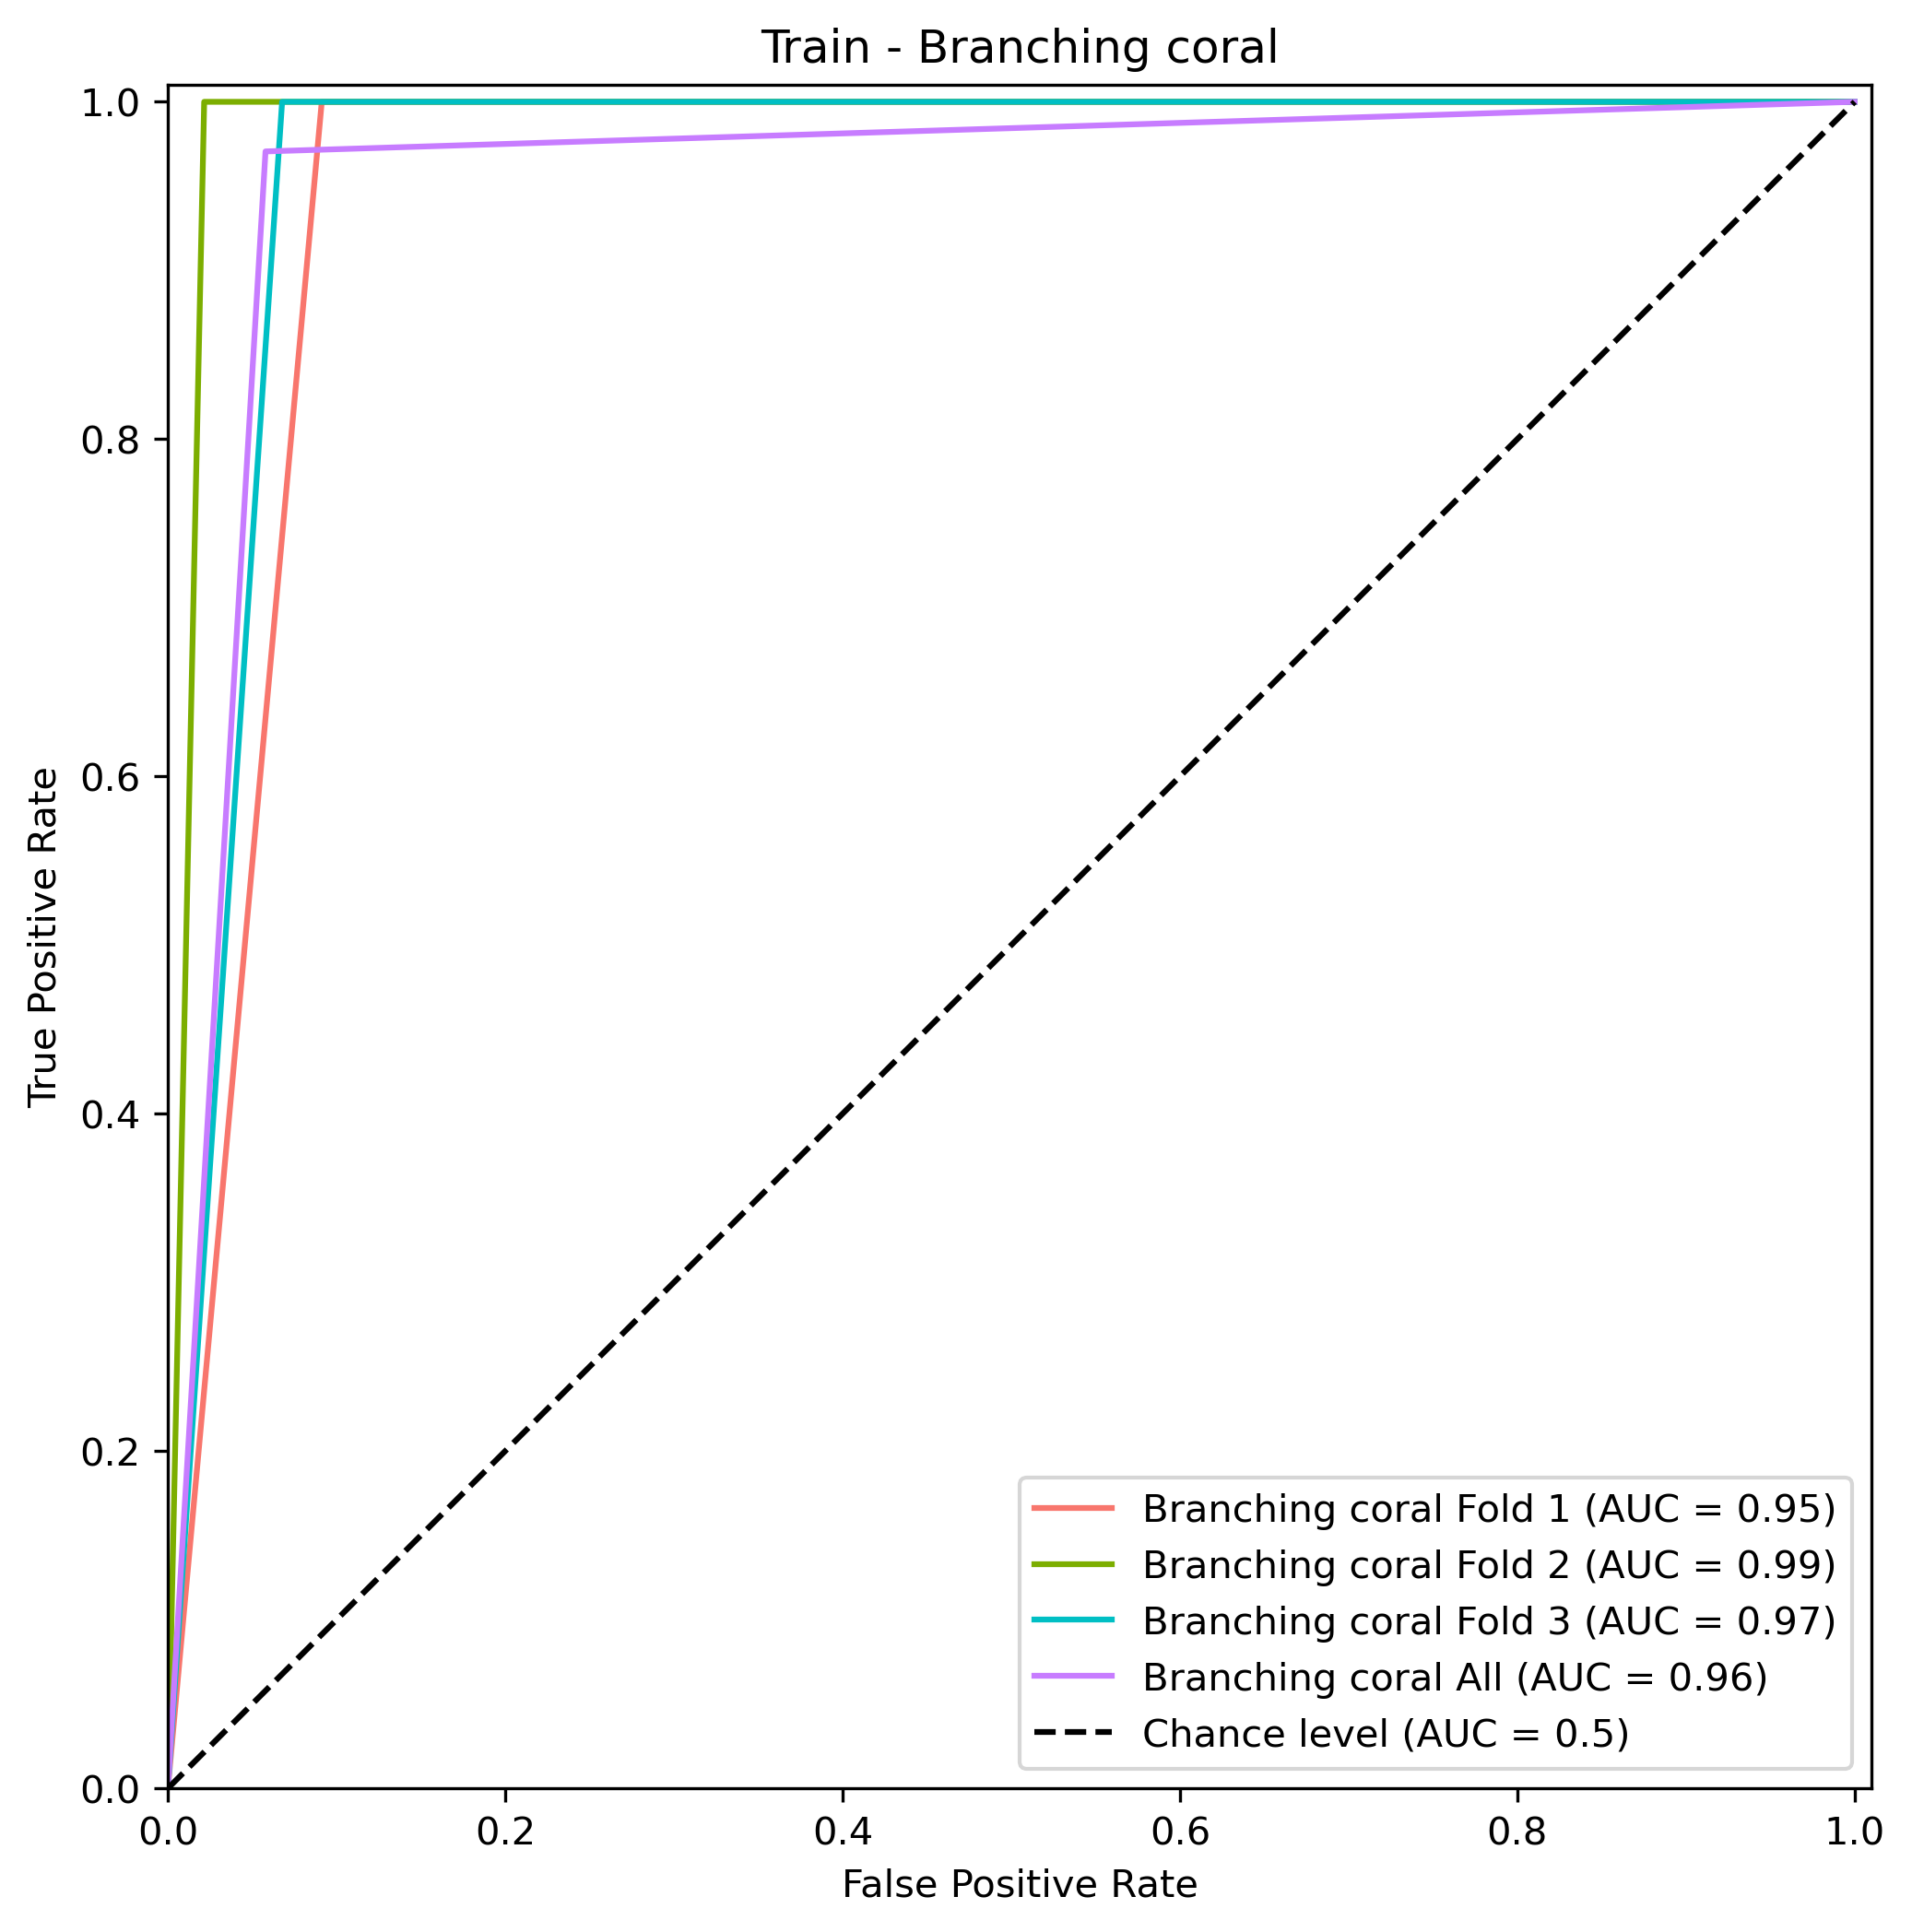
\includegraphics{03-Chapitre3/figures/supplementary/03-receiver_operator_curve_train_rf_Branching coral.png}
\caption{AUC curves of the explanatory power for the Branching
coral.}\label{fig:chap3figS8}
}
\end{figure}

\begin{figure}
\hypertarget{fig:chap3figS9}{%
\centering
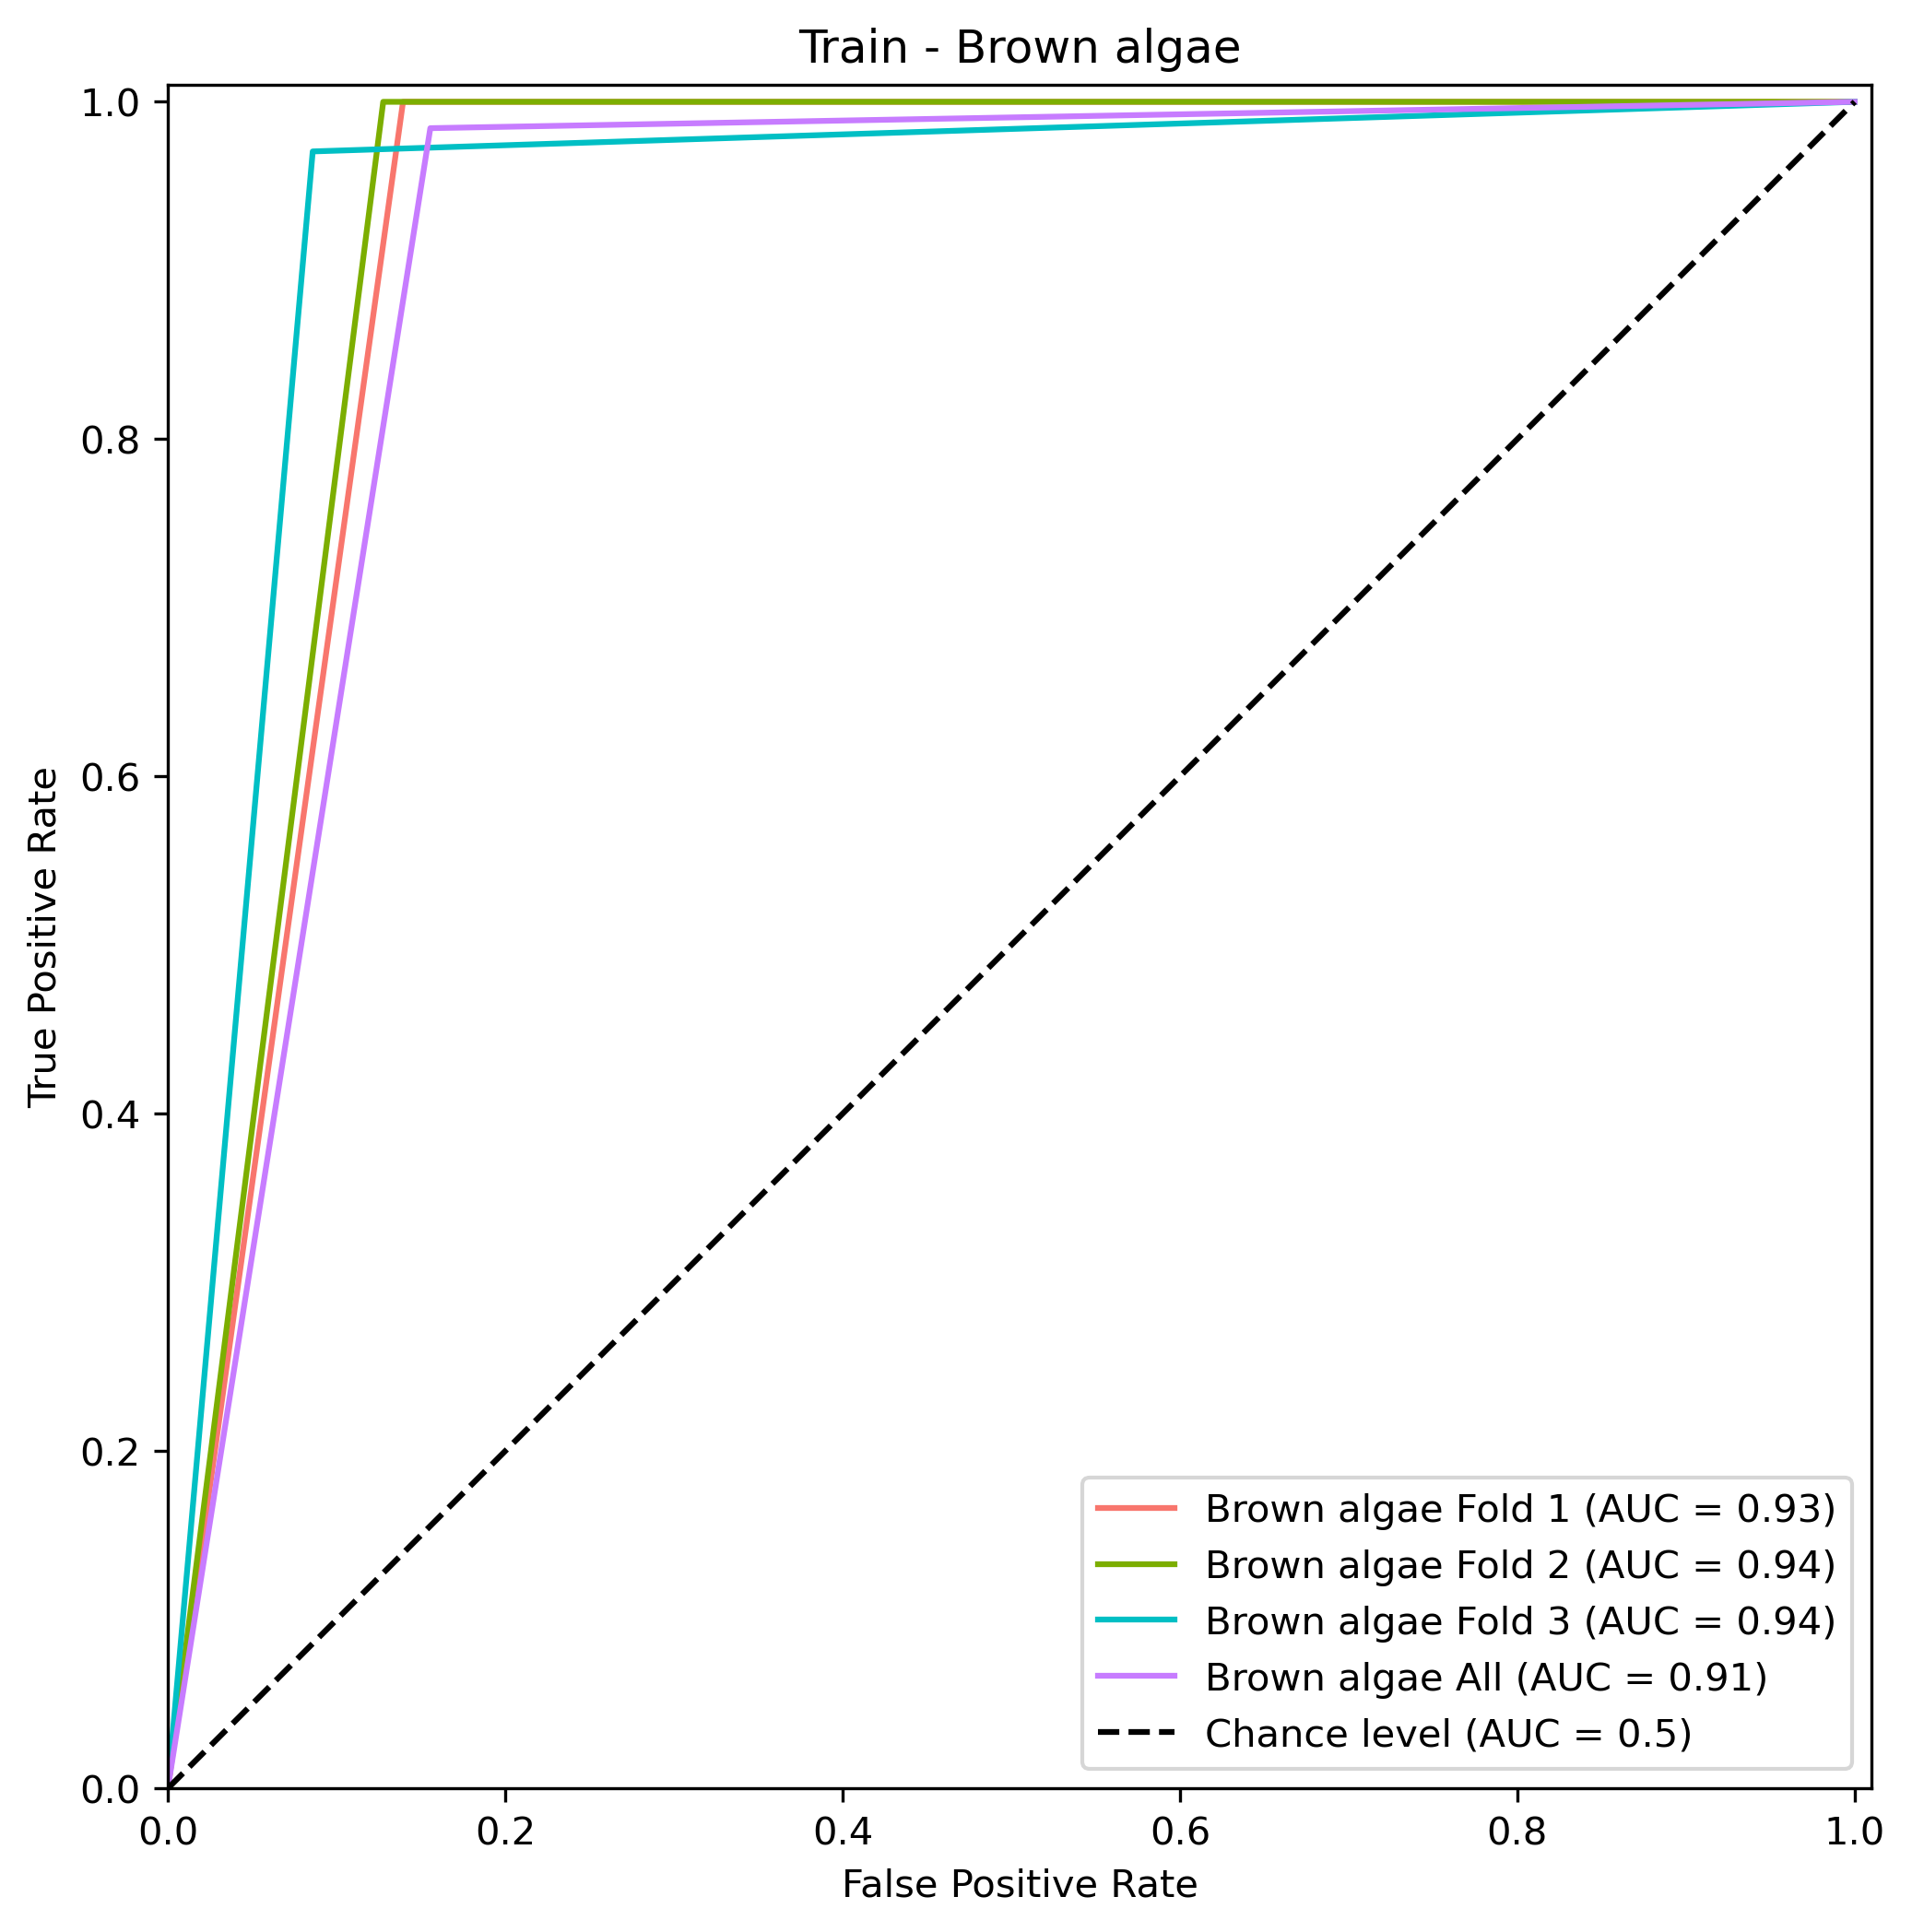
\includegraphics{03-Chapitre3/figures/supplementary/03-receiver_operator_curve_train_rf_Brown algae.png}
\caption{AUC curves of the explanatory power for the Brown
algae.}\label{fig:chap3figS9}
}
\end{figure}

\begin{figure}
\hypertarget{fig:chap3figS10}{%
\centering
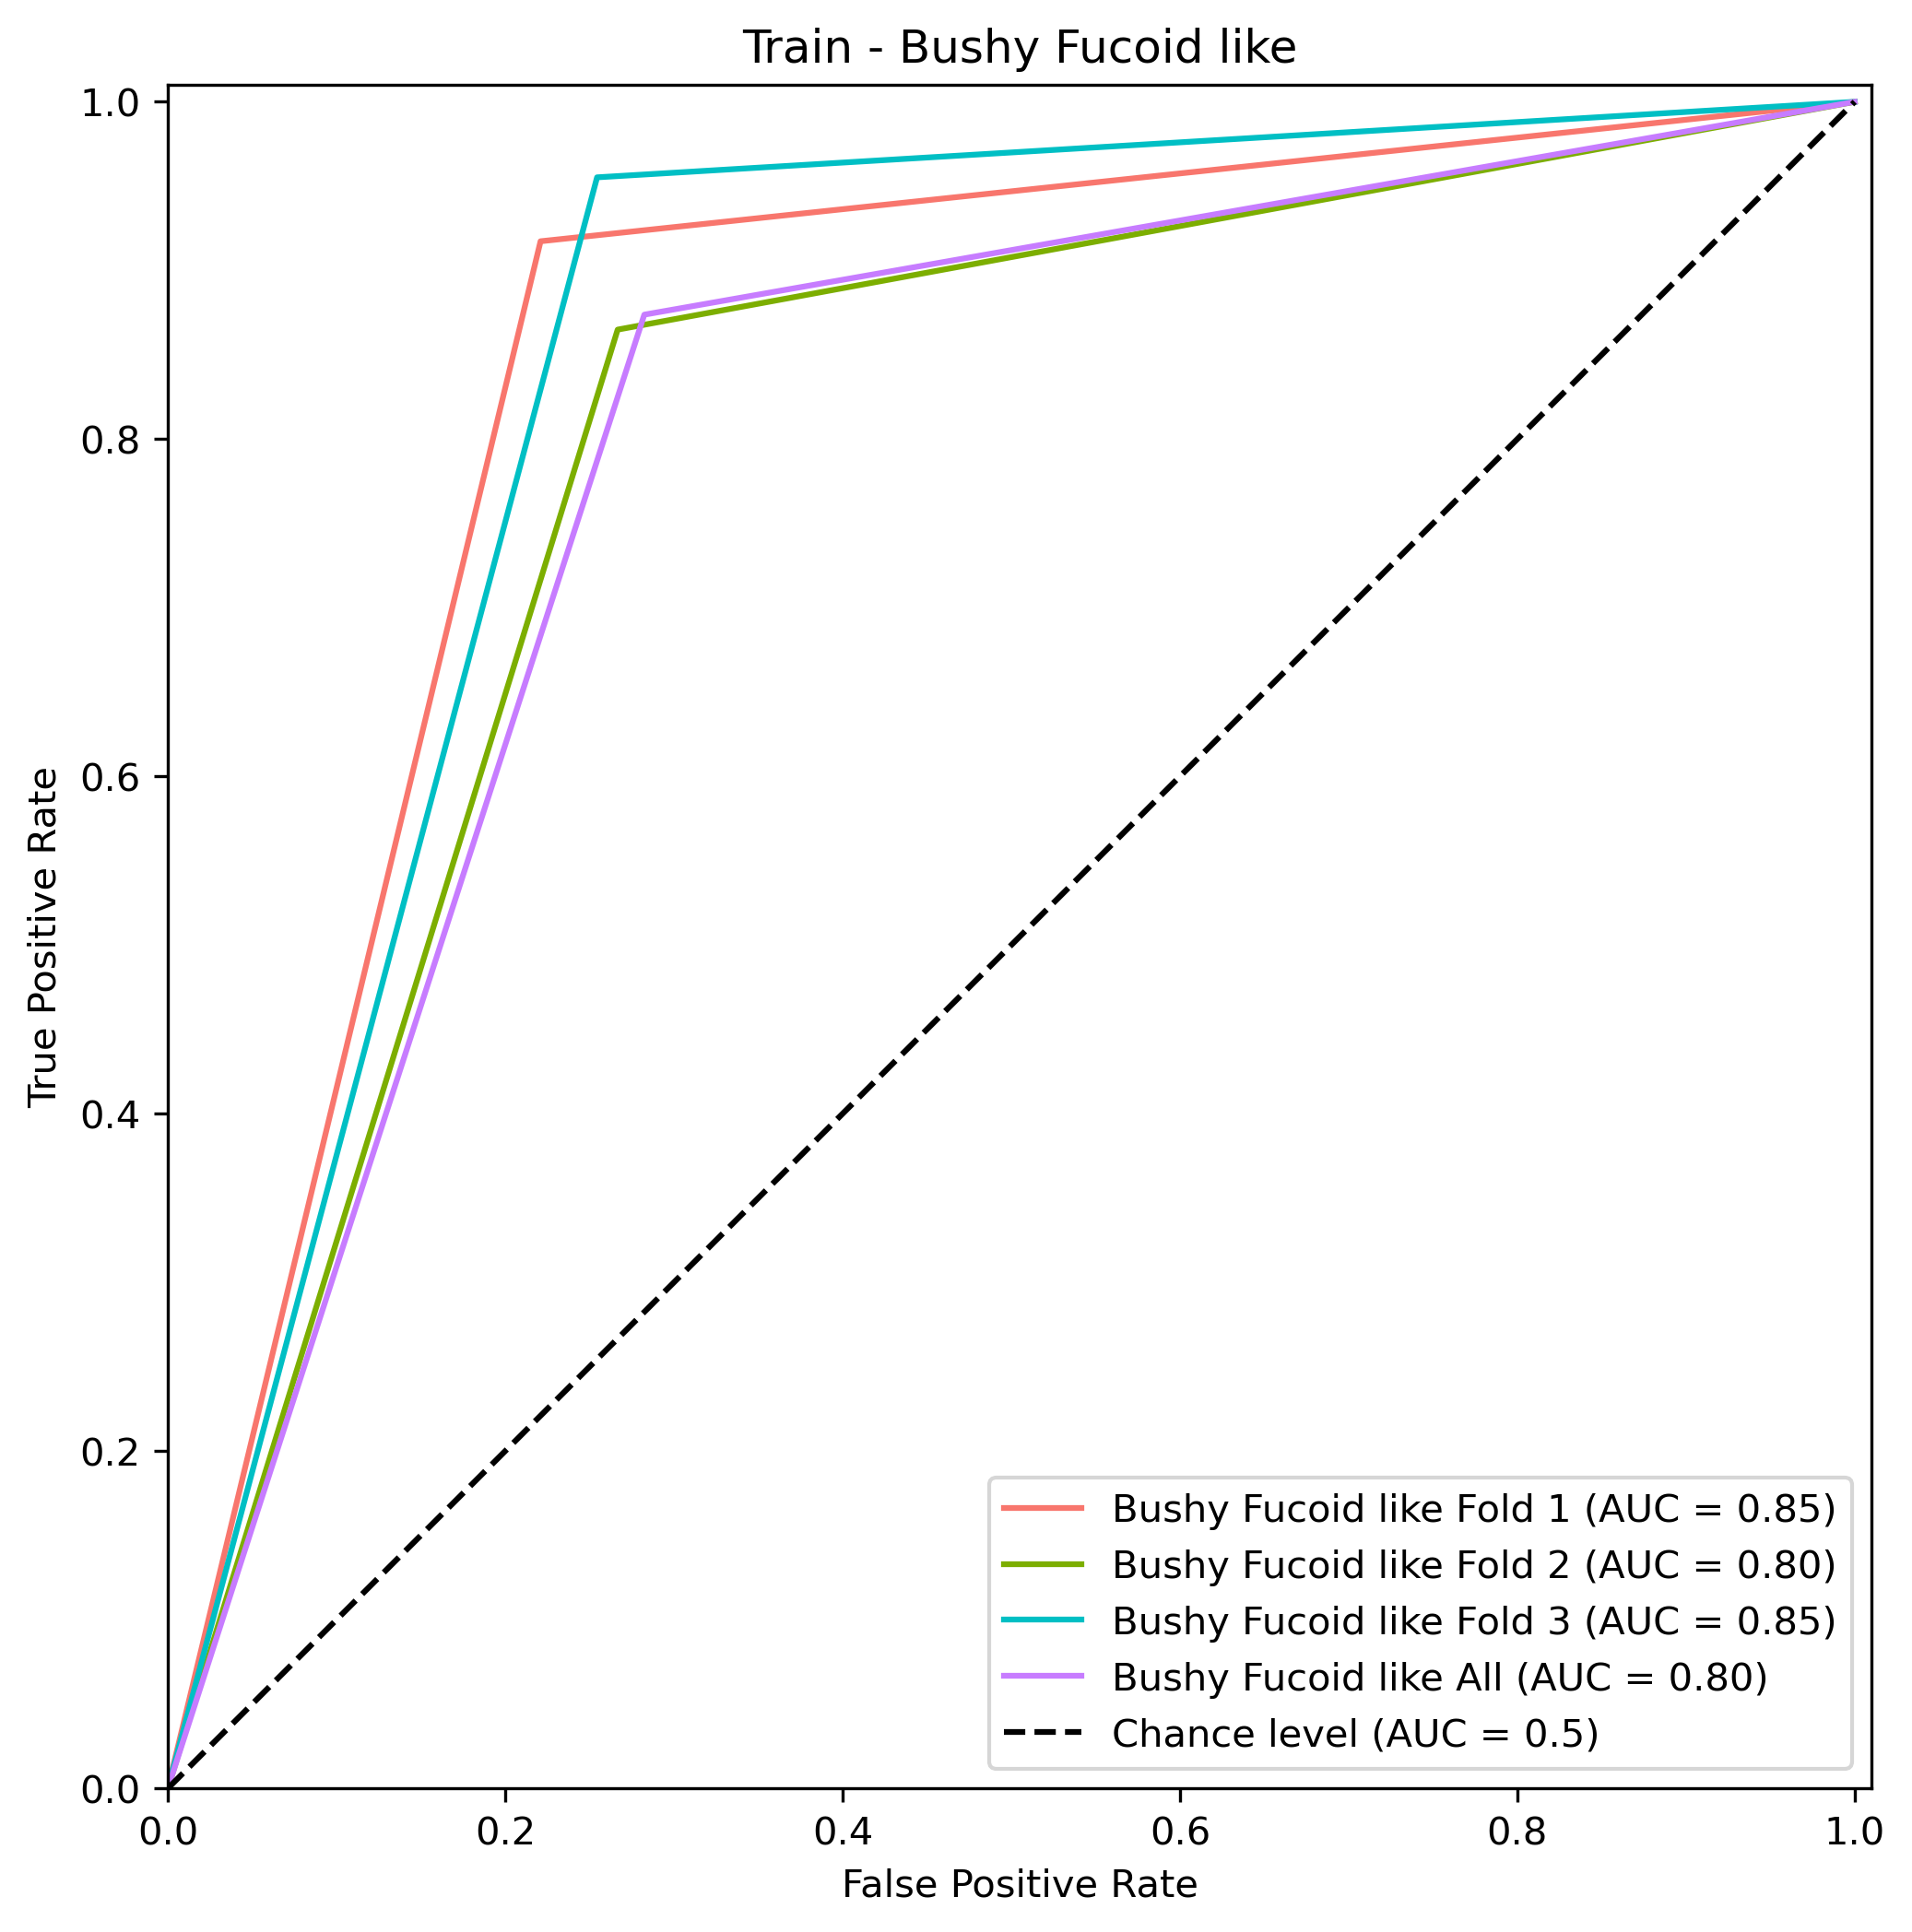
\includegraphics{03-Chapitre3/figures/supplementary/03-receiver_operator_curve_train_rf_Bushy Fucoid like.png}
\caption{AUC curves of the explanatory power for the Bushy Fucoid
like.}\label{fig:chap3figS10}
}
\end{figure}

\begin{figure}
\hypertarget{fig:chap3figS11}{%
\centering
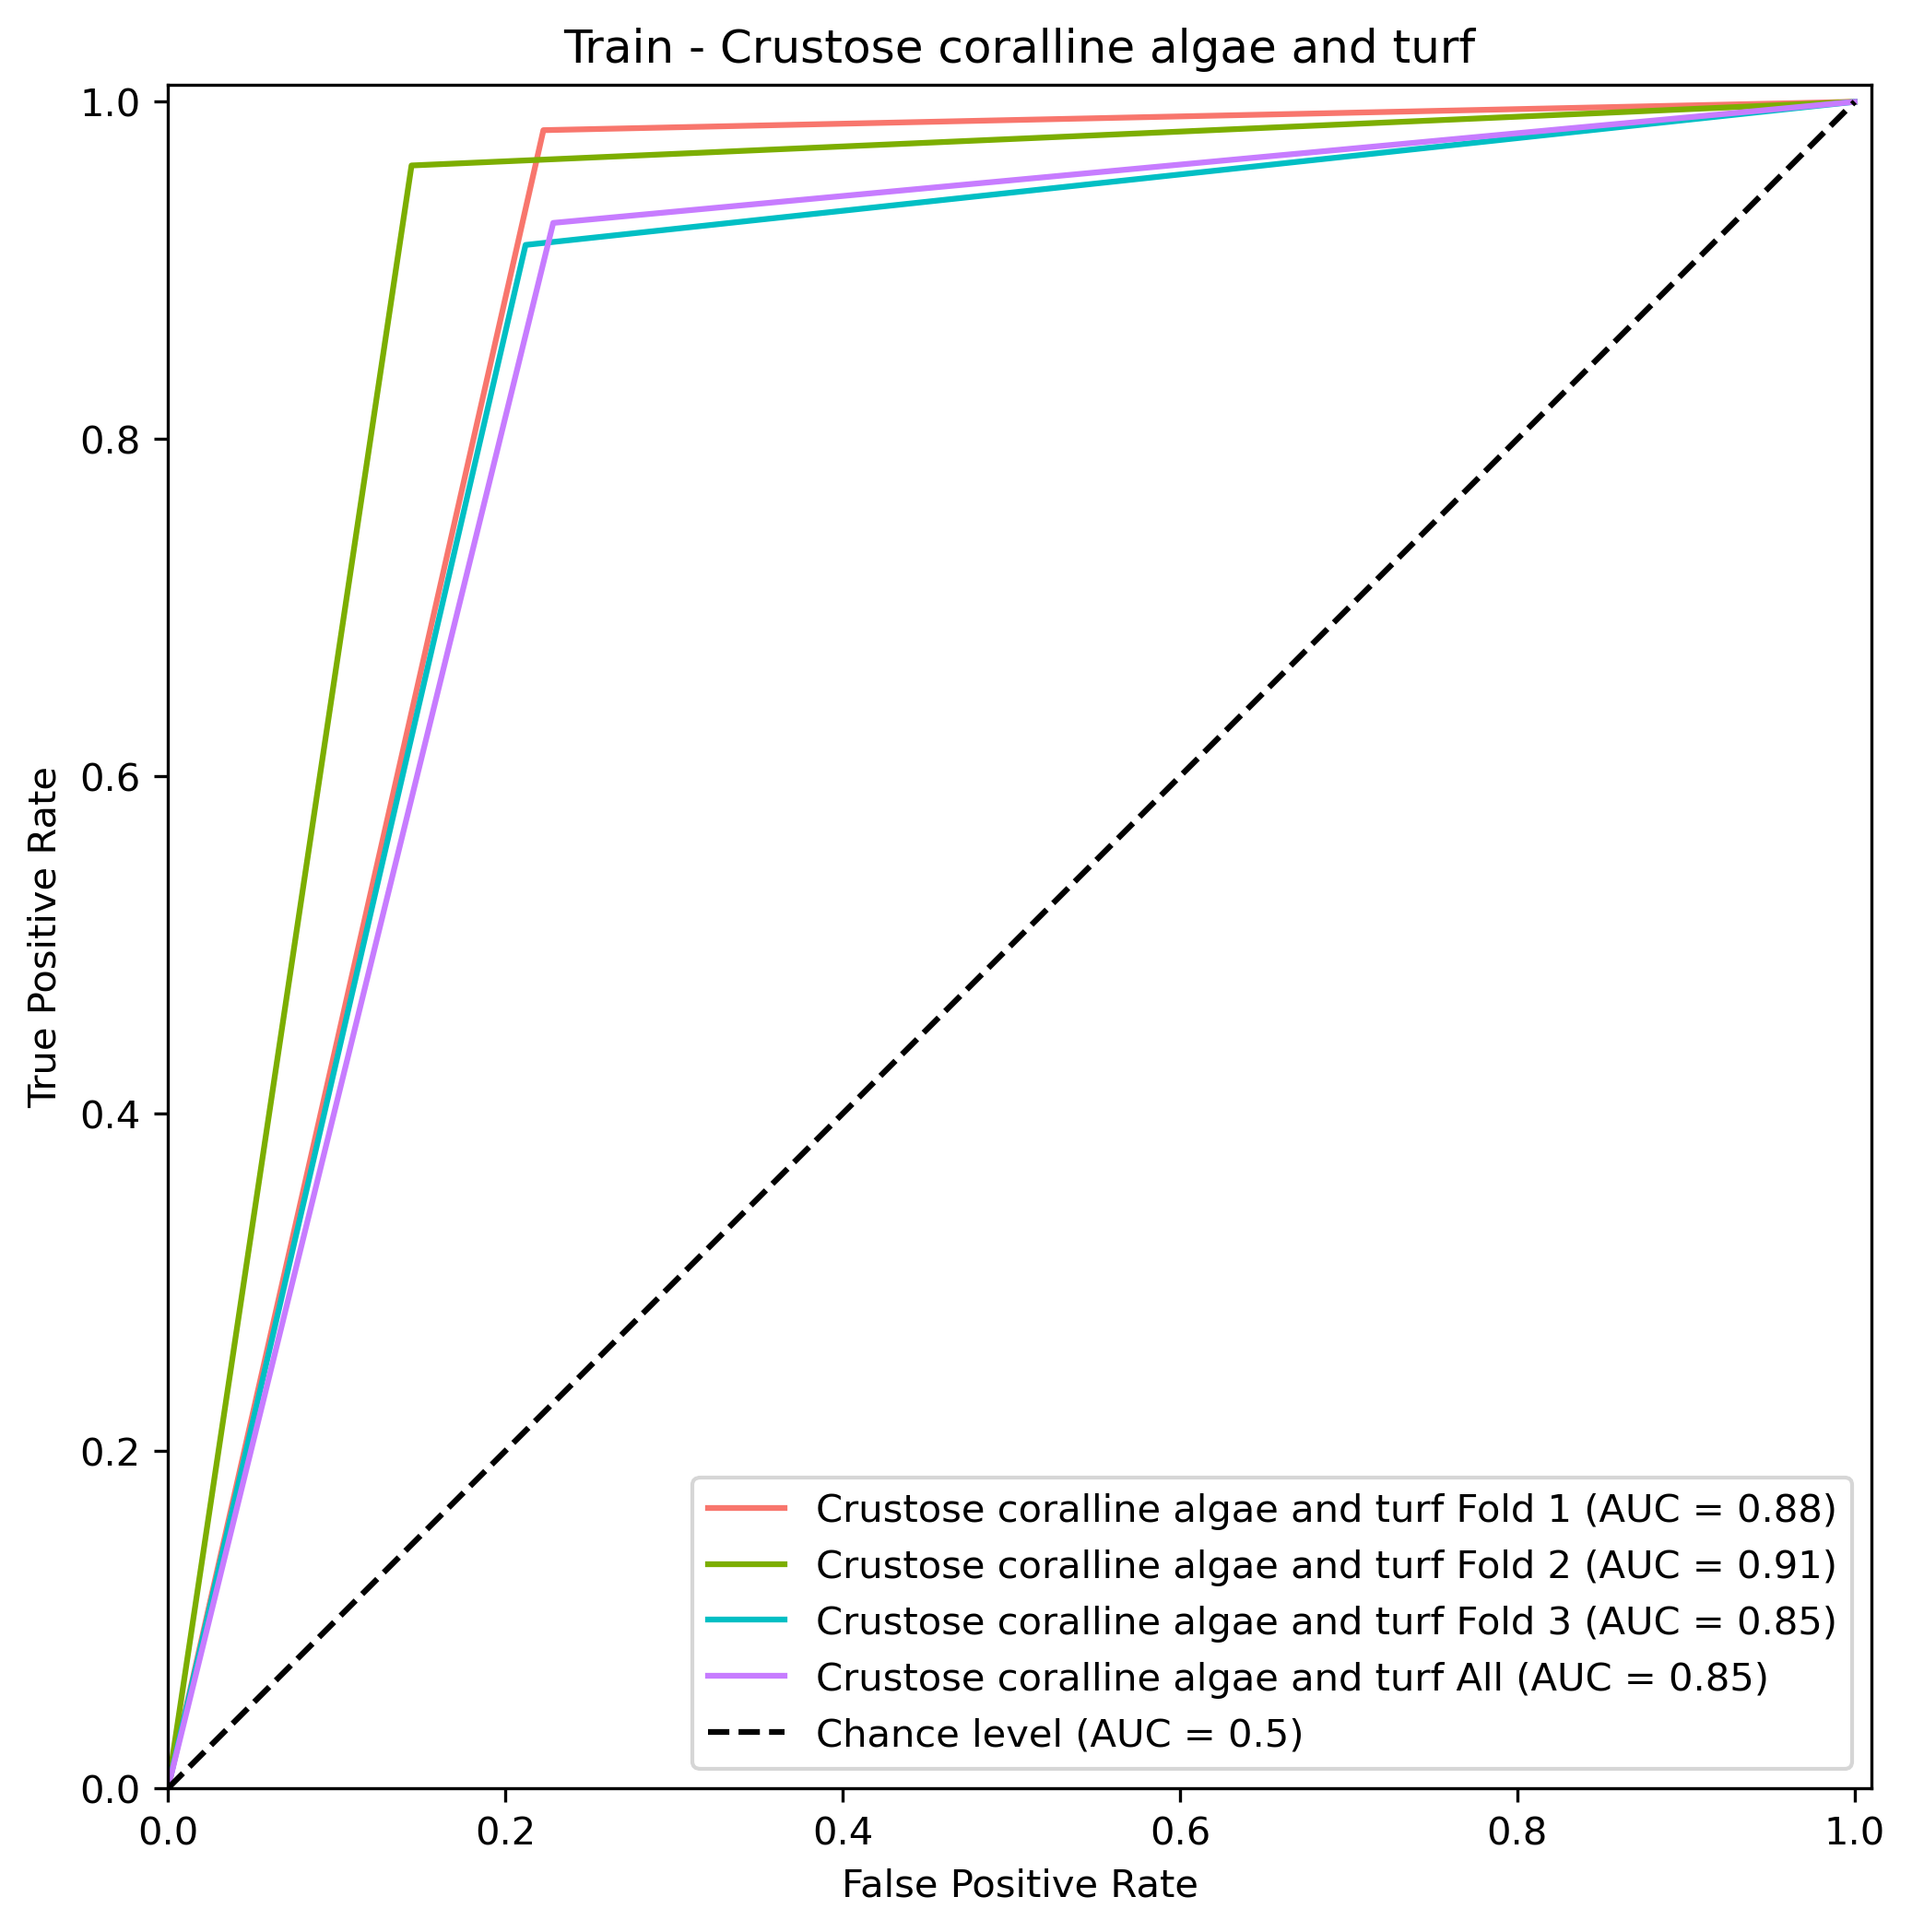
\includegraphics{03-Chapitre3/figures/supplementary/03-receiver_operator_curve_train_rf_Crustose coralline algae and turf.png}
\caption{AUC curves of the explanatory power for the Crustose coralline
algae and turf.}\label{fig:chap3figS11}
}
\end{figure}

\begin{figure}
\hypertarget{fig:chap3figS12}{%
\centering
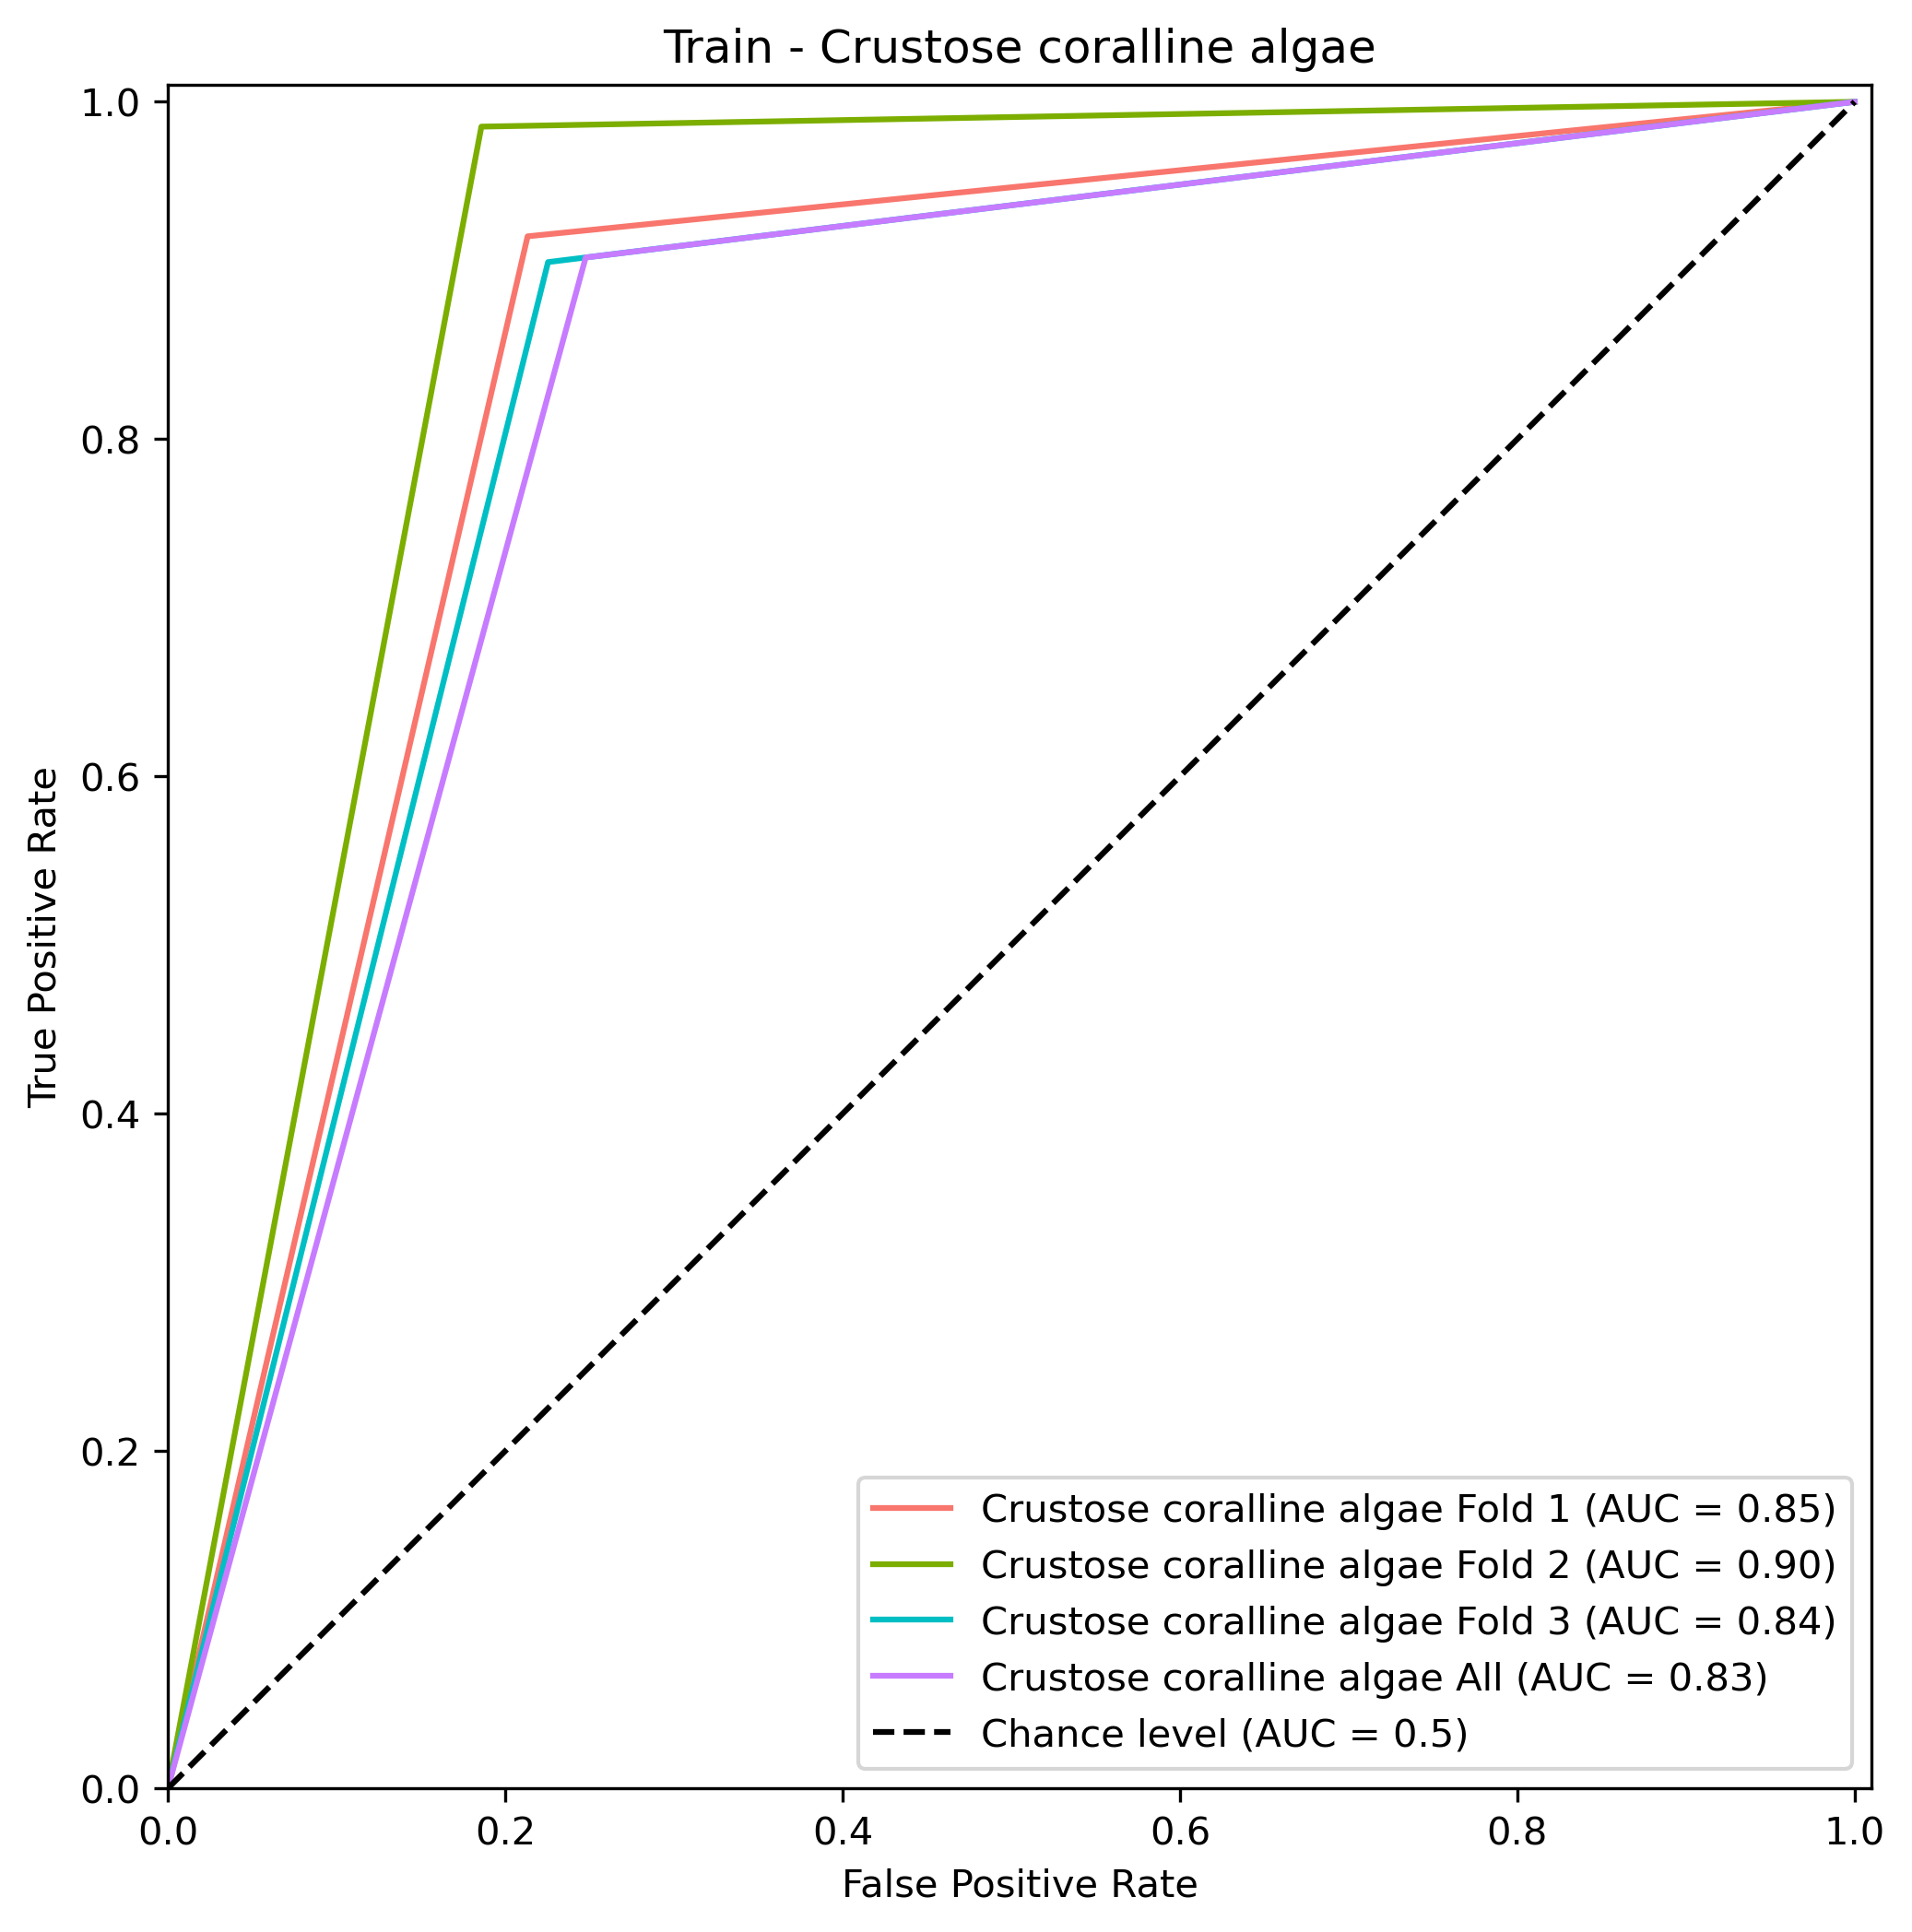
\includegraphics{03-Chapitre3/figures/supplementary/03-receiver_operator_curve_train_rf_Crustose coralline algae.png}
\caption{AUC curves of the explanatory power for the Crustose coralline
algae.}\label{fig:chap3figS12}
}
\end{figure}

\begin{figure}
\hypertarget{fig:chap3figS13}{%
\centering
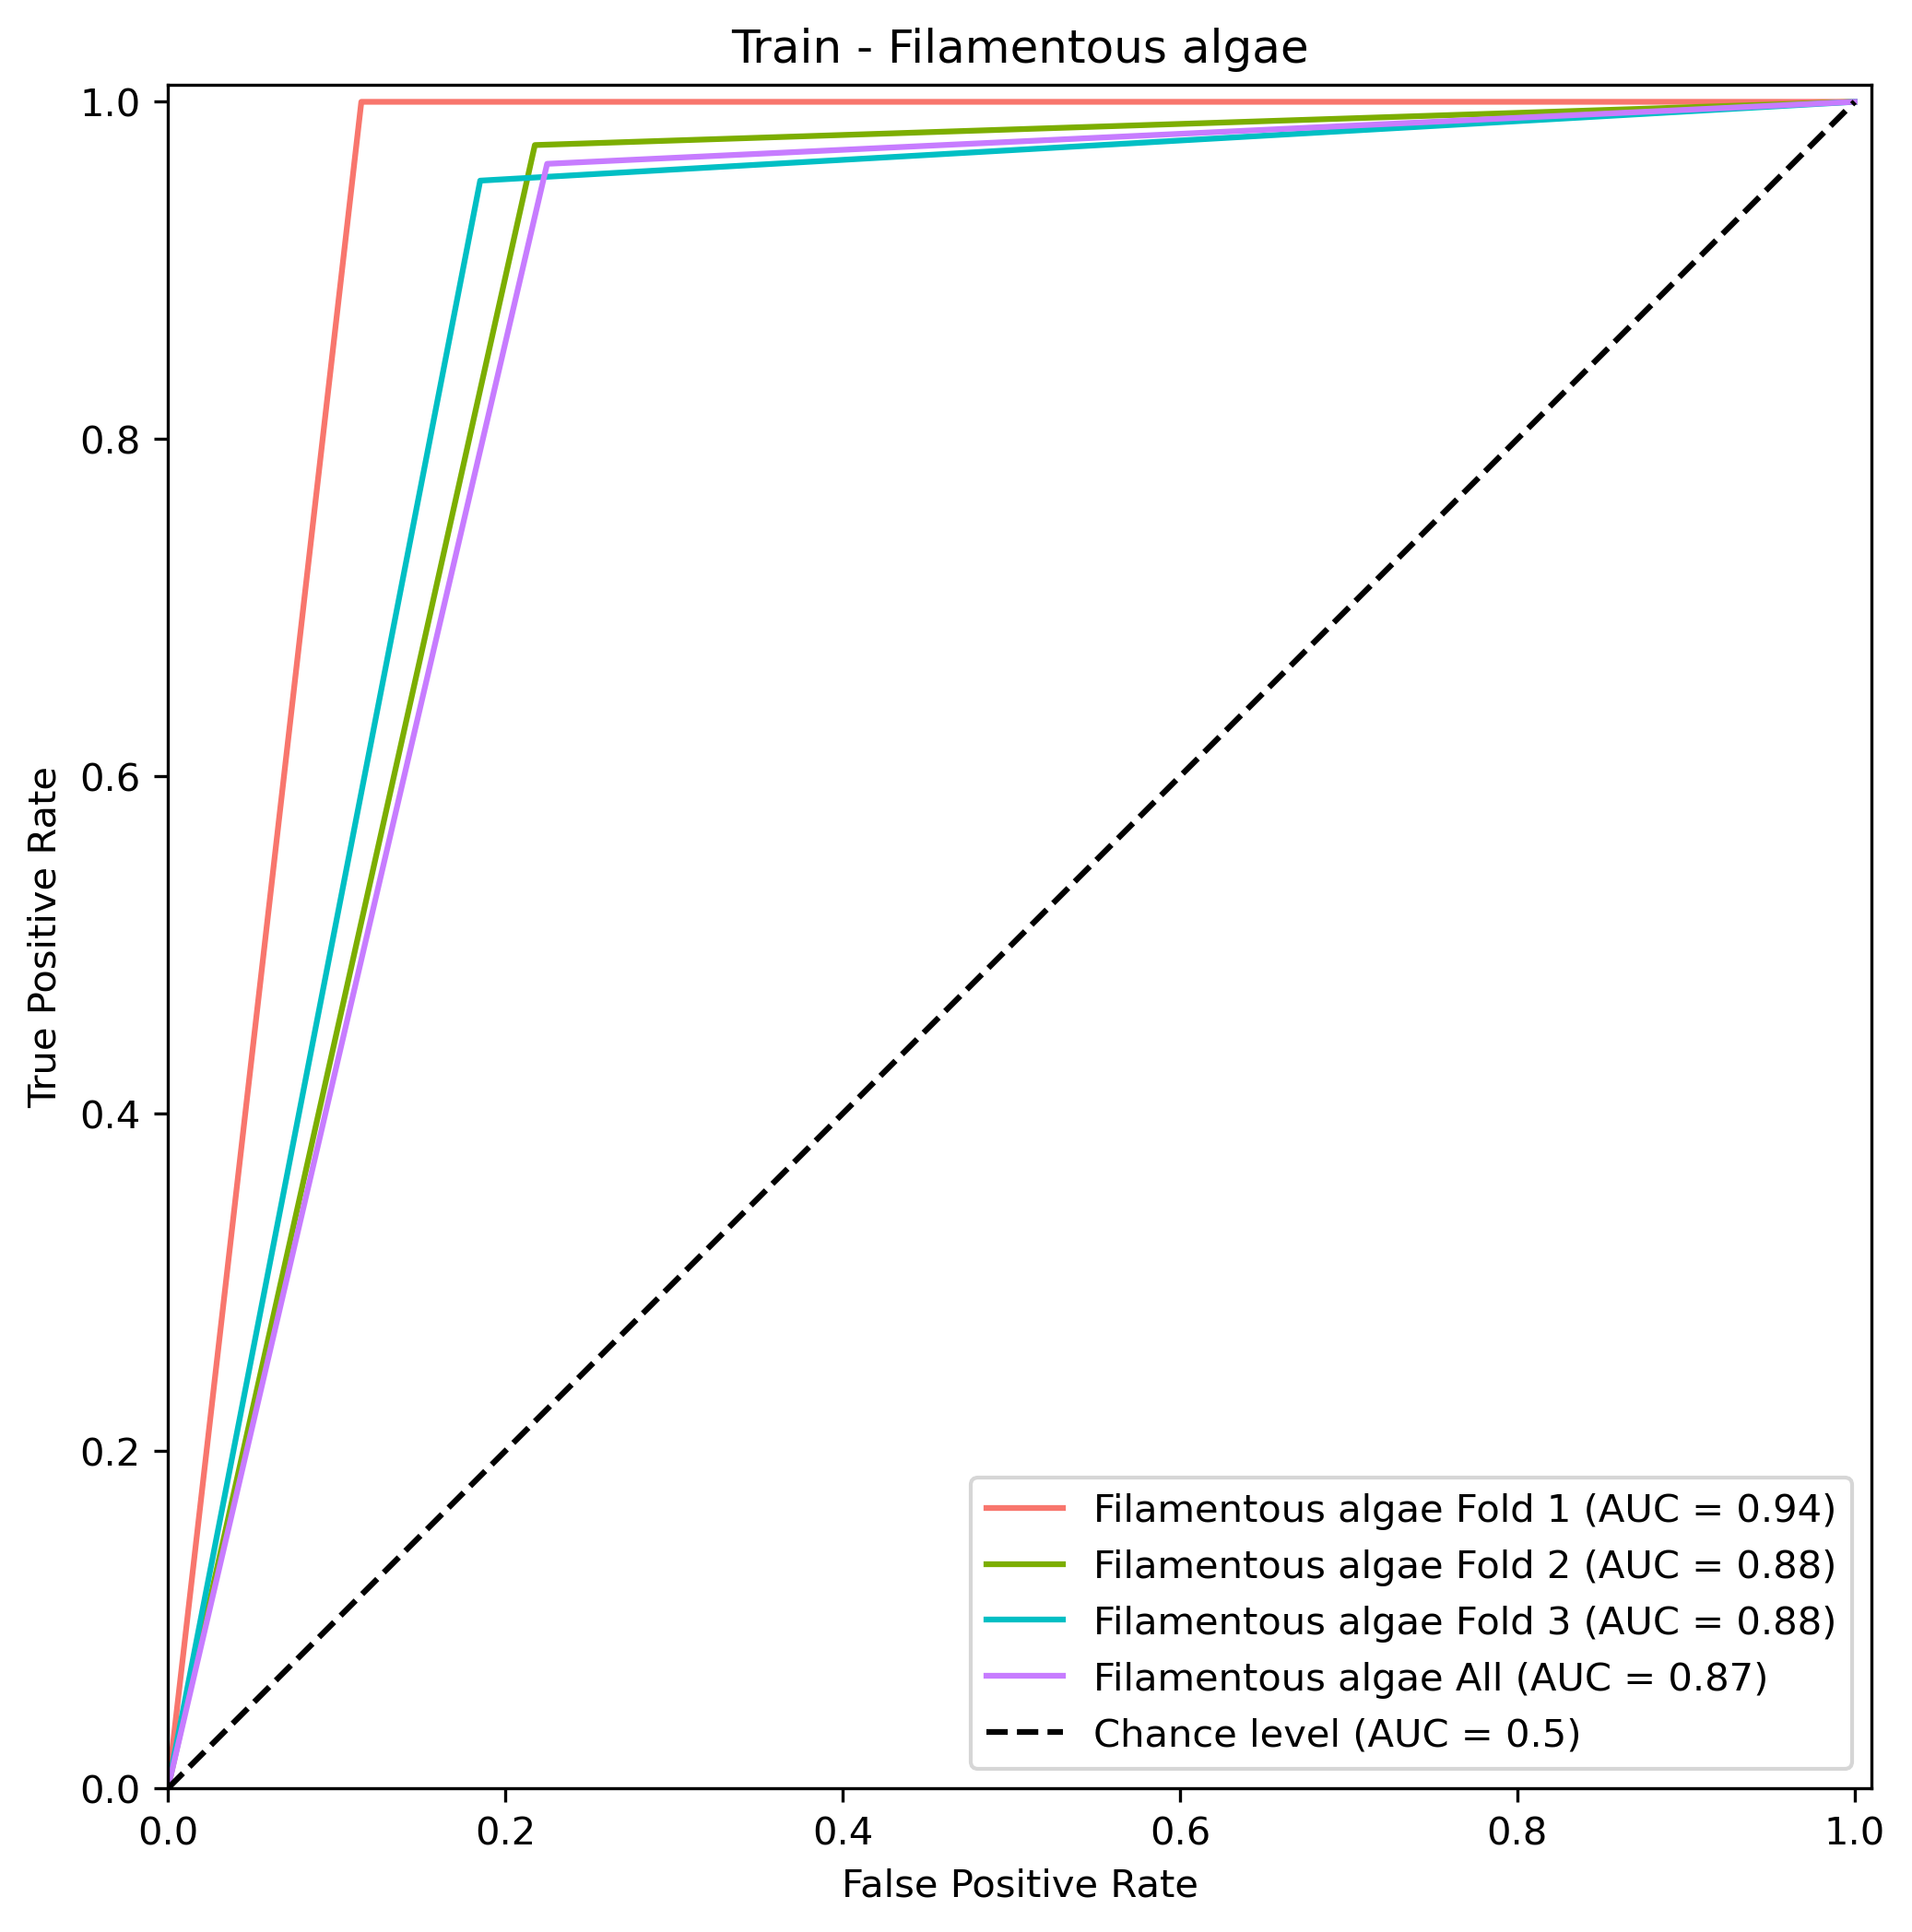
\includegraphics{03-Chapitre3/figures/supplementary/03-receiver_operator_curve_train_rf_Filamentous algae.png}
\caption{AUC curves of the explanatory power for the Filamentous
algae.}\label{fig:chap3figS13}
}
\end{figure}

\begin{figure}
\hypertarget{fig:chap3figS14}{%
\centering
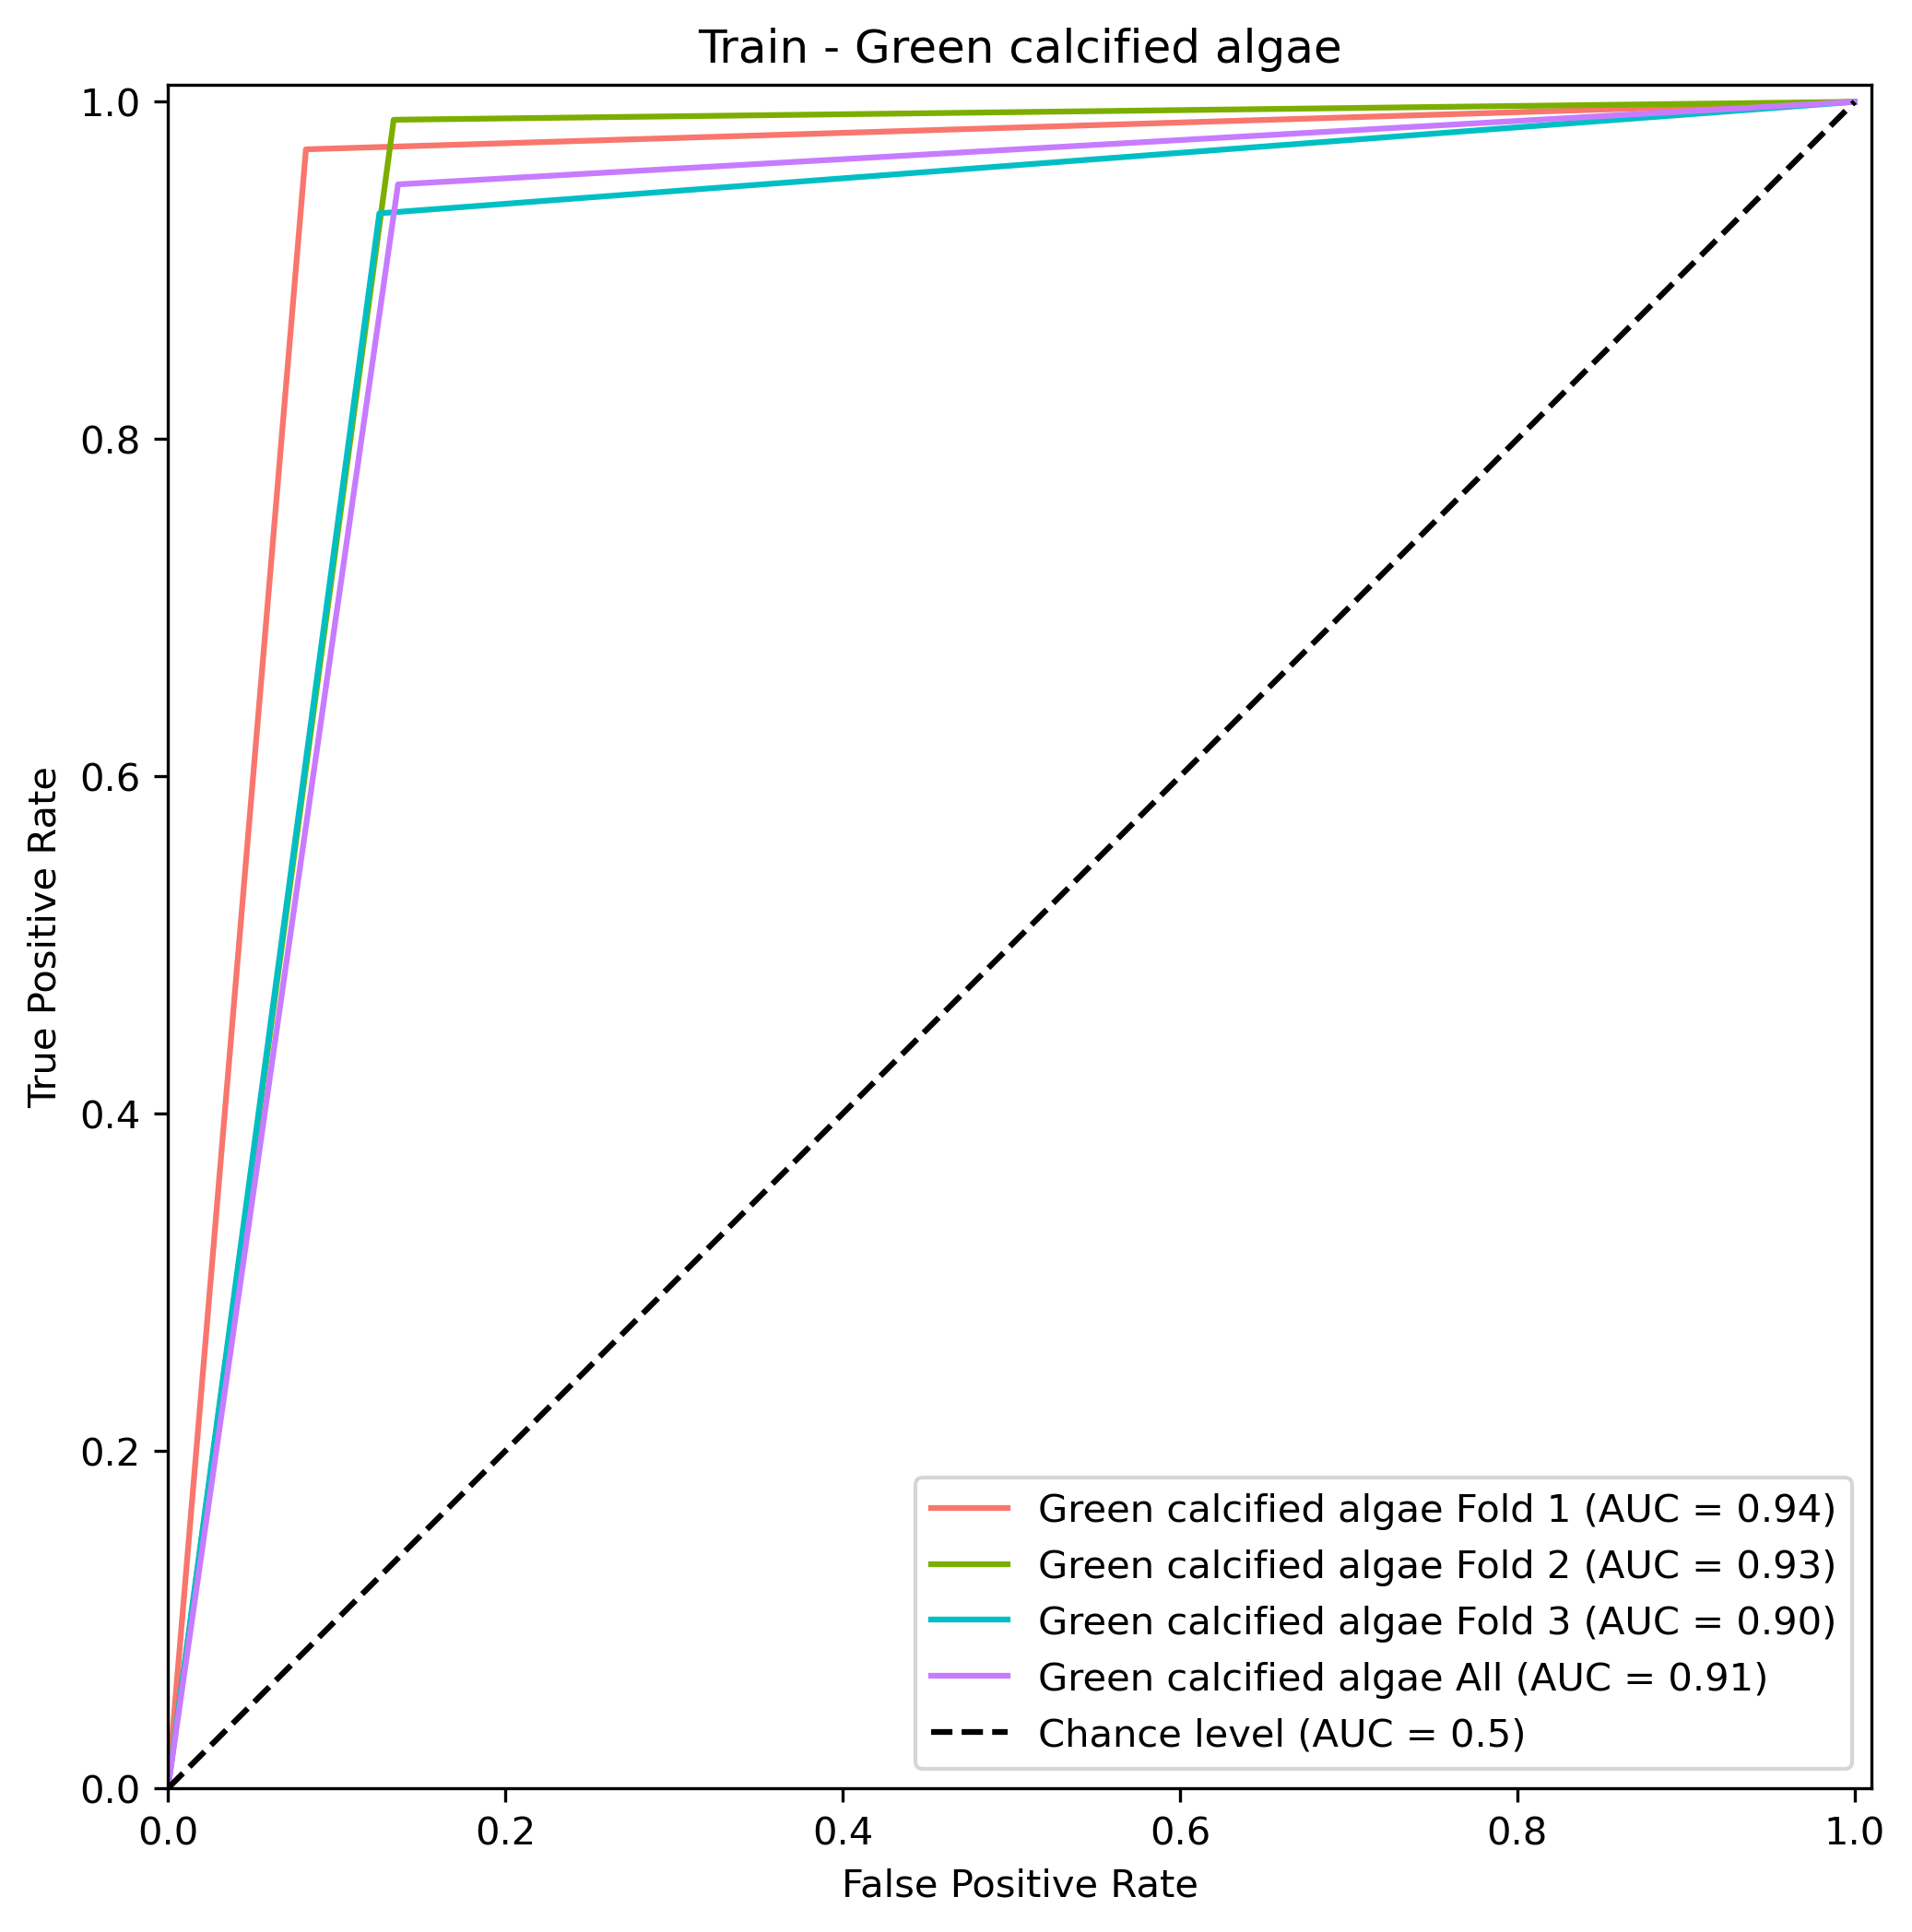
\includegraphics{03-Chapitre3/figures/supplementary/03-receiver_operator_curve_train_rf_Green calcified algae.png}
\caption{AUC curves of the explanatory power for the Green Calcified
algae.}\label{fig:chap3figS14}
}
\end{figure}

\begin{figure}
\hypertarget{fig:chap3figS15}{%
\centering
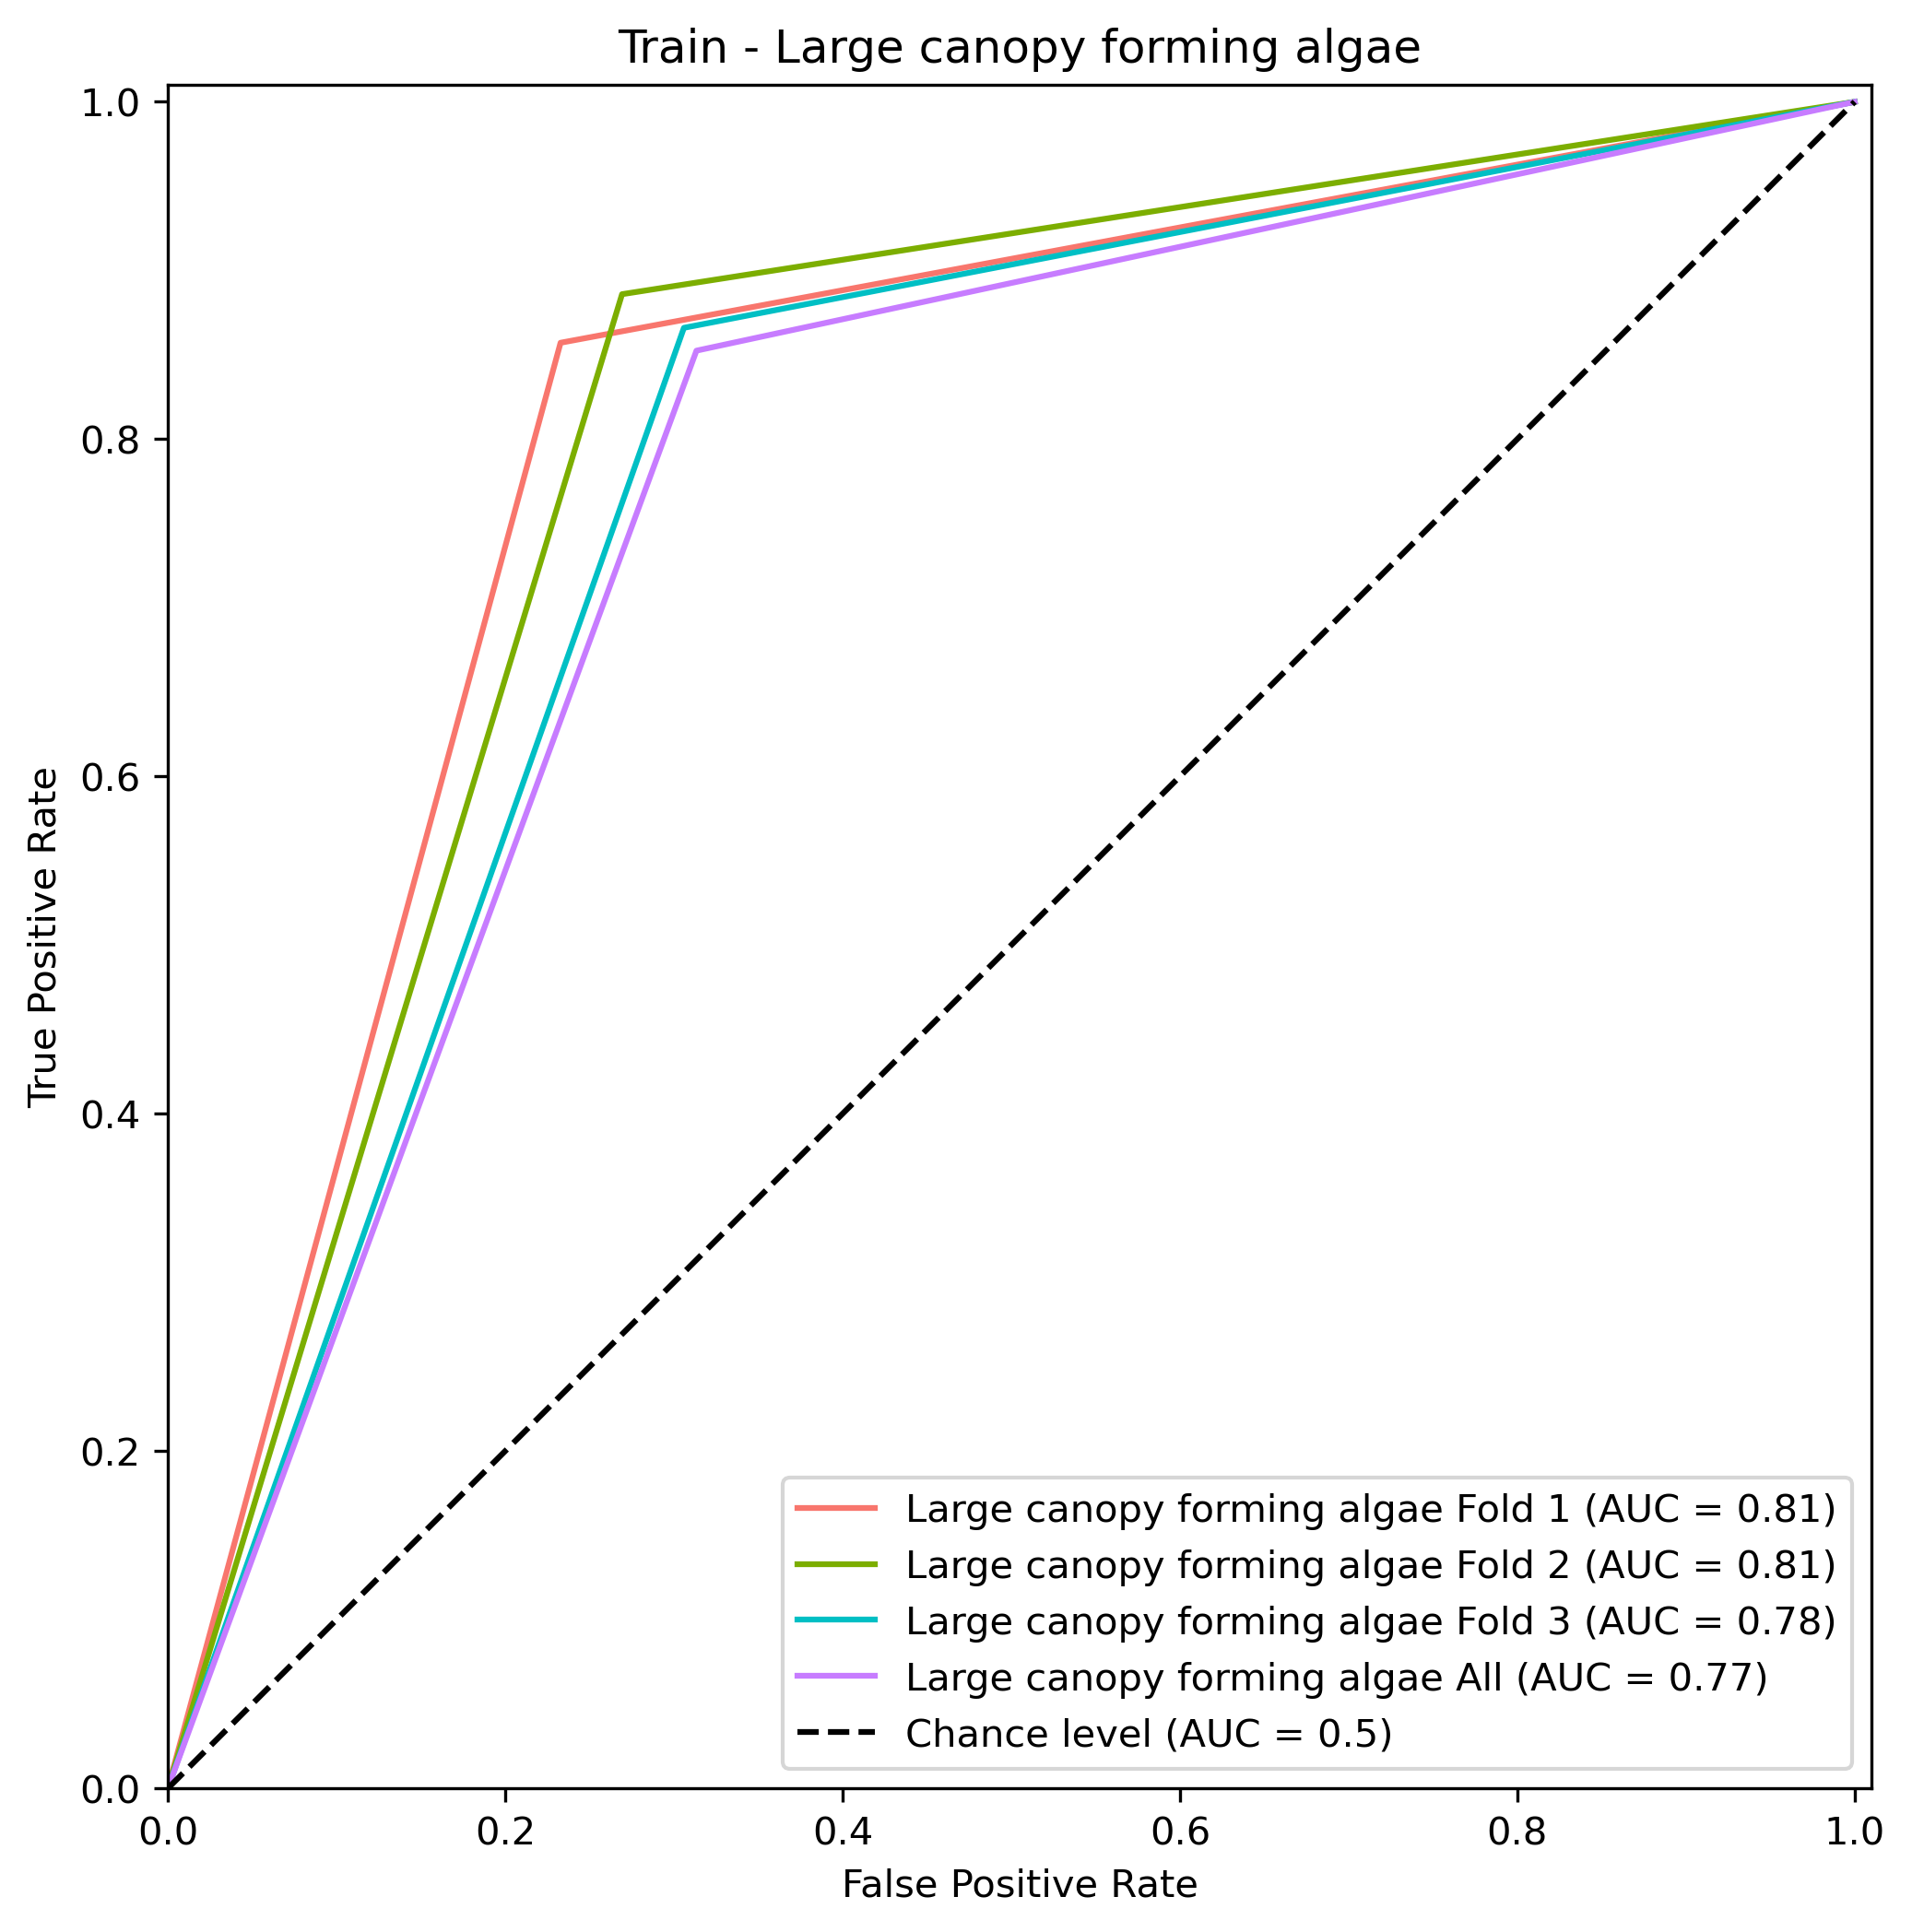
\includegraphics{03-Chapitre3/figures/supplementary/03-receiver_operator_curve_train_rf_Large canopy forming algae.png}
\caption{AUC curves of the explanatory power for the Large canopy
forming algae.}\label{fig:chap3figS15}
}
\end{figure}

\begin{figure}
\hypertarget{fig:chap3figS16}{%
\centering
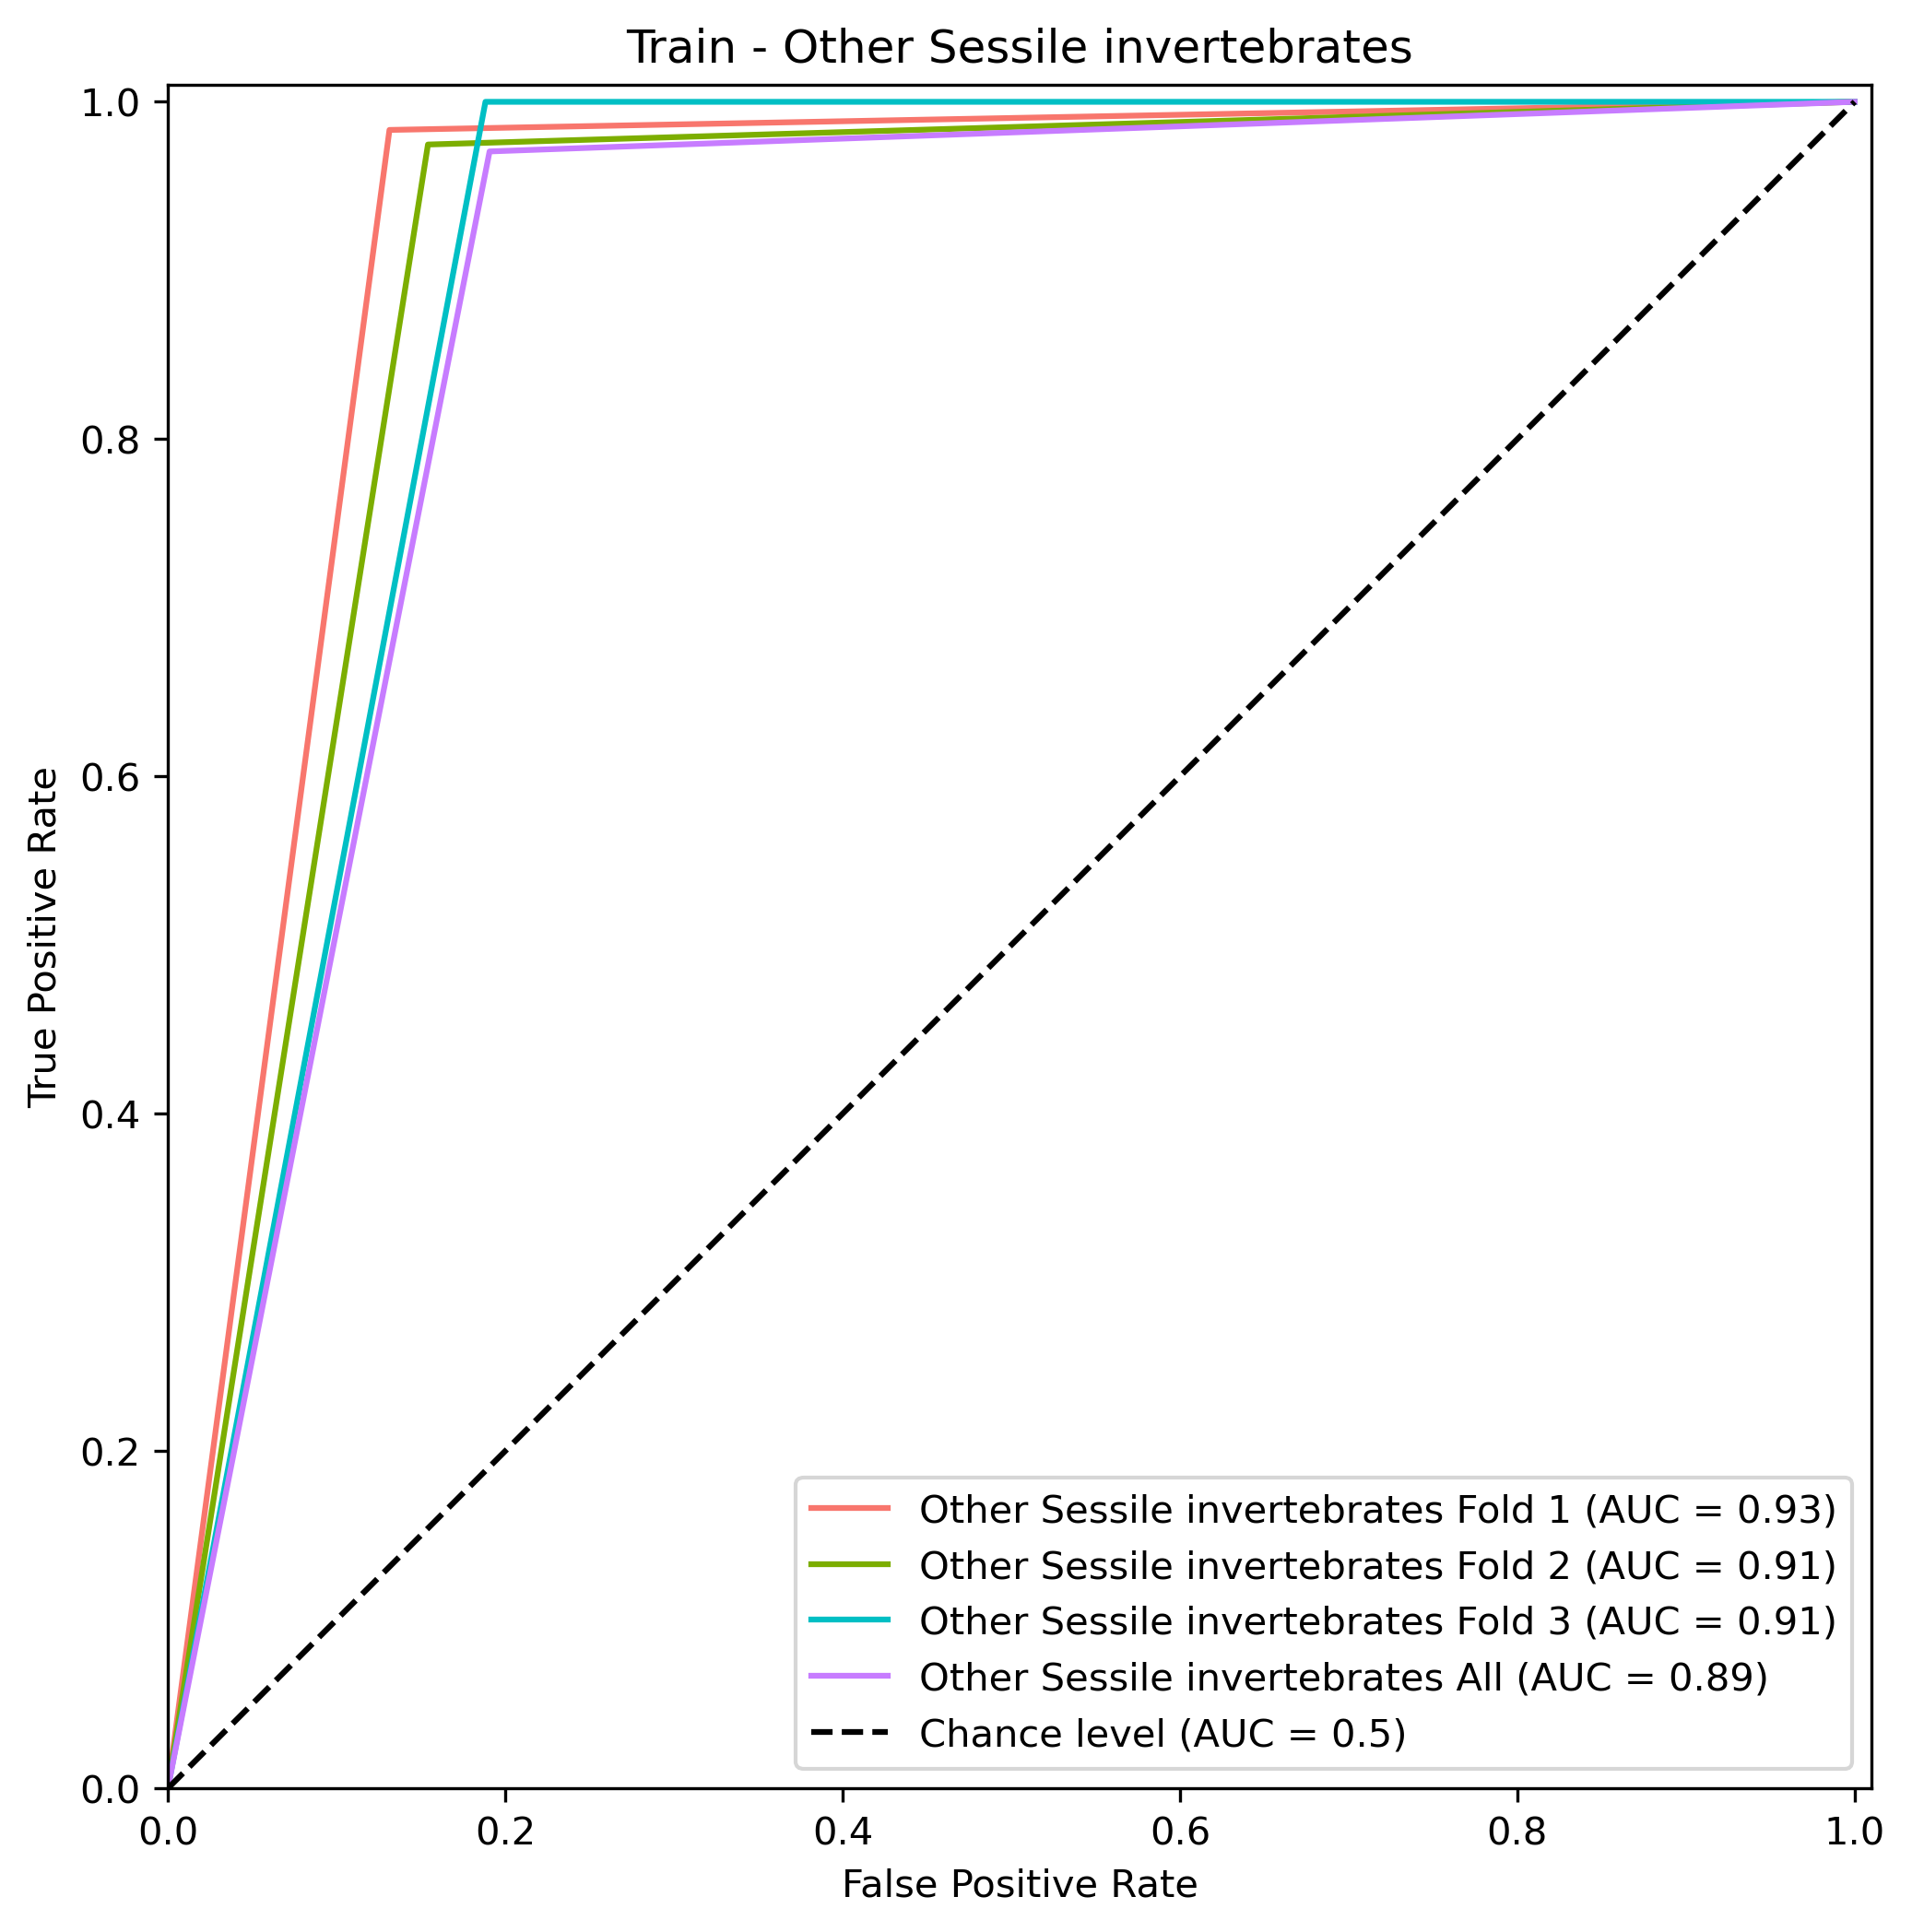
\includegraphics{03-Chapitre3/figures/supplementary/03-receiver_operator_curve_train_rf_Other Sessile invertebrates.png}
\caption{AUC curves of the explanatory power for the Other Sessile
invertebrates.}\label{fig:chap3figS16}
}
\end{figure}

\begin{figure}
\hypertarget{fig:chap3figS17}{%
\centering
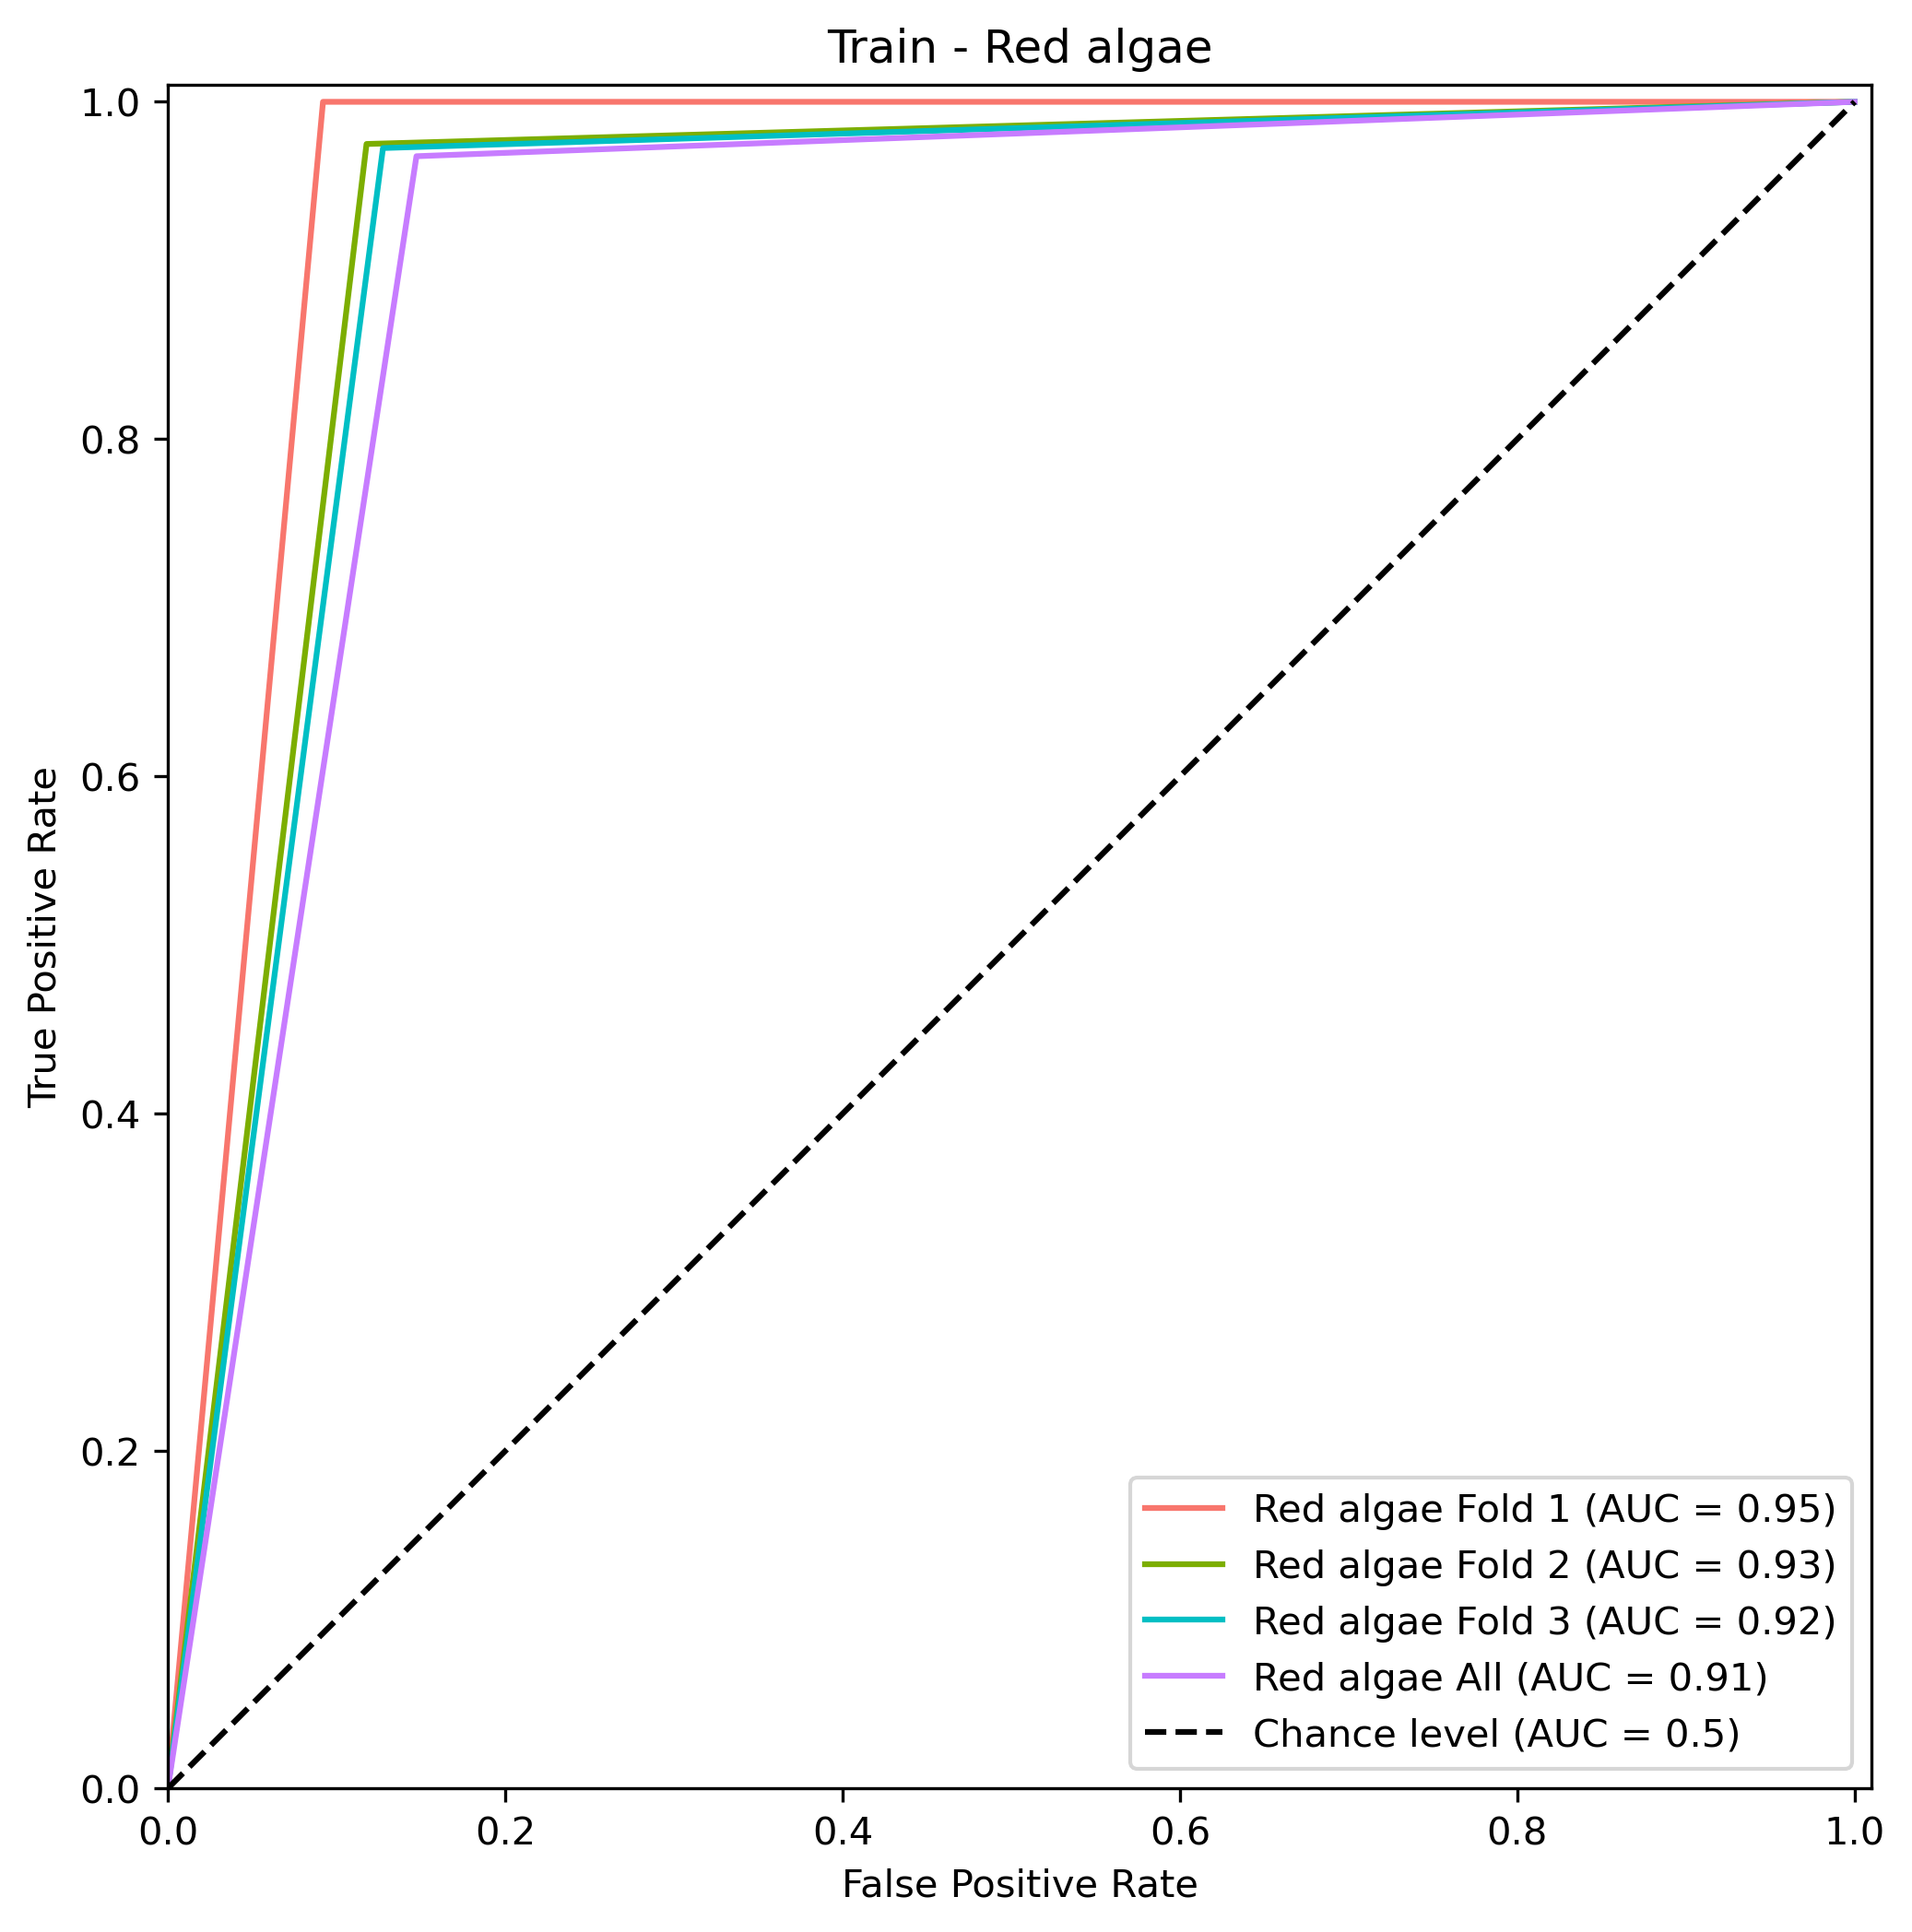
\includegraphics{03-Chapitre3/figures/supplementary/03-receiver_operator_curve_train_rf_Red algae.png}
\caption{AUC curves of the explanatory power for the Red
algae.}\label{fig:chap3figS17}
}
\end{figure}

\begin{figure}
\hypertarget{fig:chap3figS18}{%
\centering
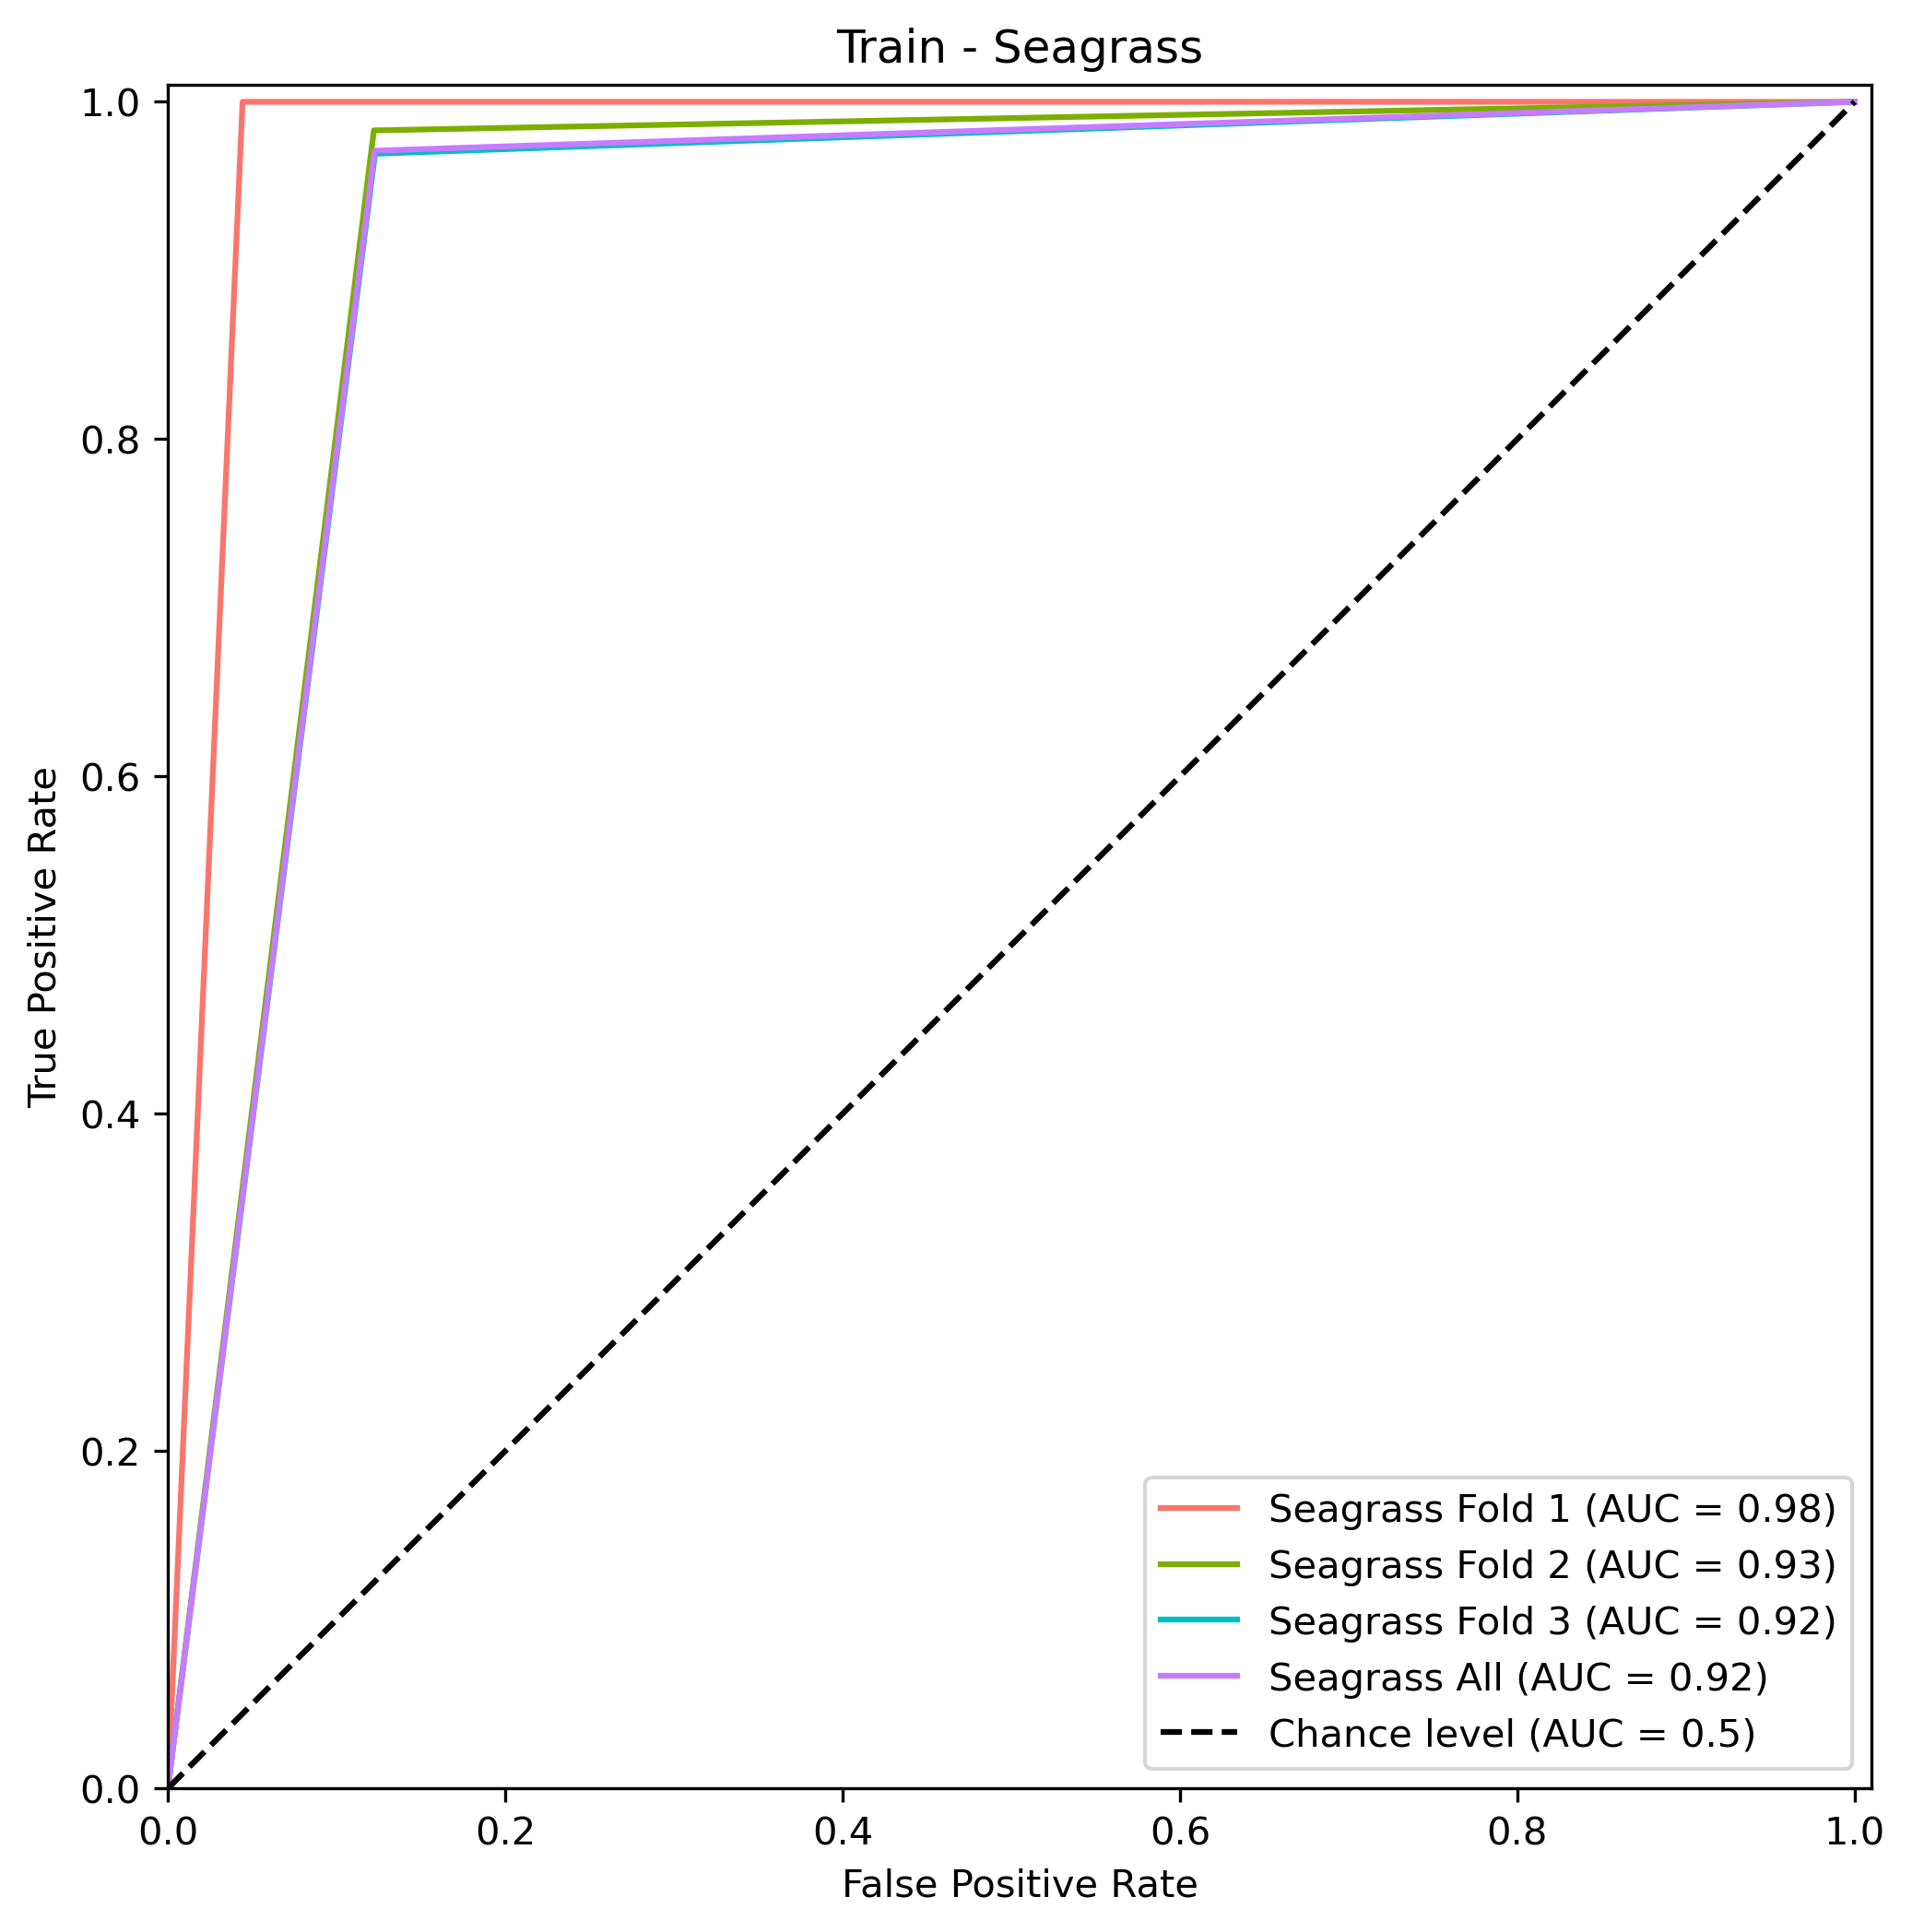
\includegraphics{03-Chapitre3/figures/supplementary/03-receiver_operator_curve_train_rf_Seagrass.png}
\caption{AUC curves of the explanatory power for the
Seagrass.}\label{fig:chap3figS18}
}
\end{figure}

\begin{figure}
\hypertarget{fig:chap3figS19}{%
\centering
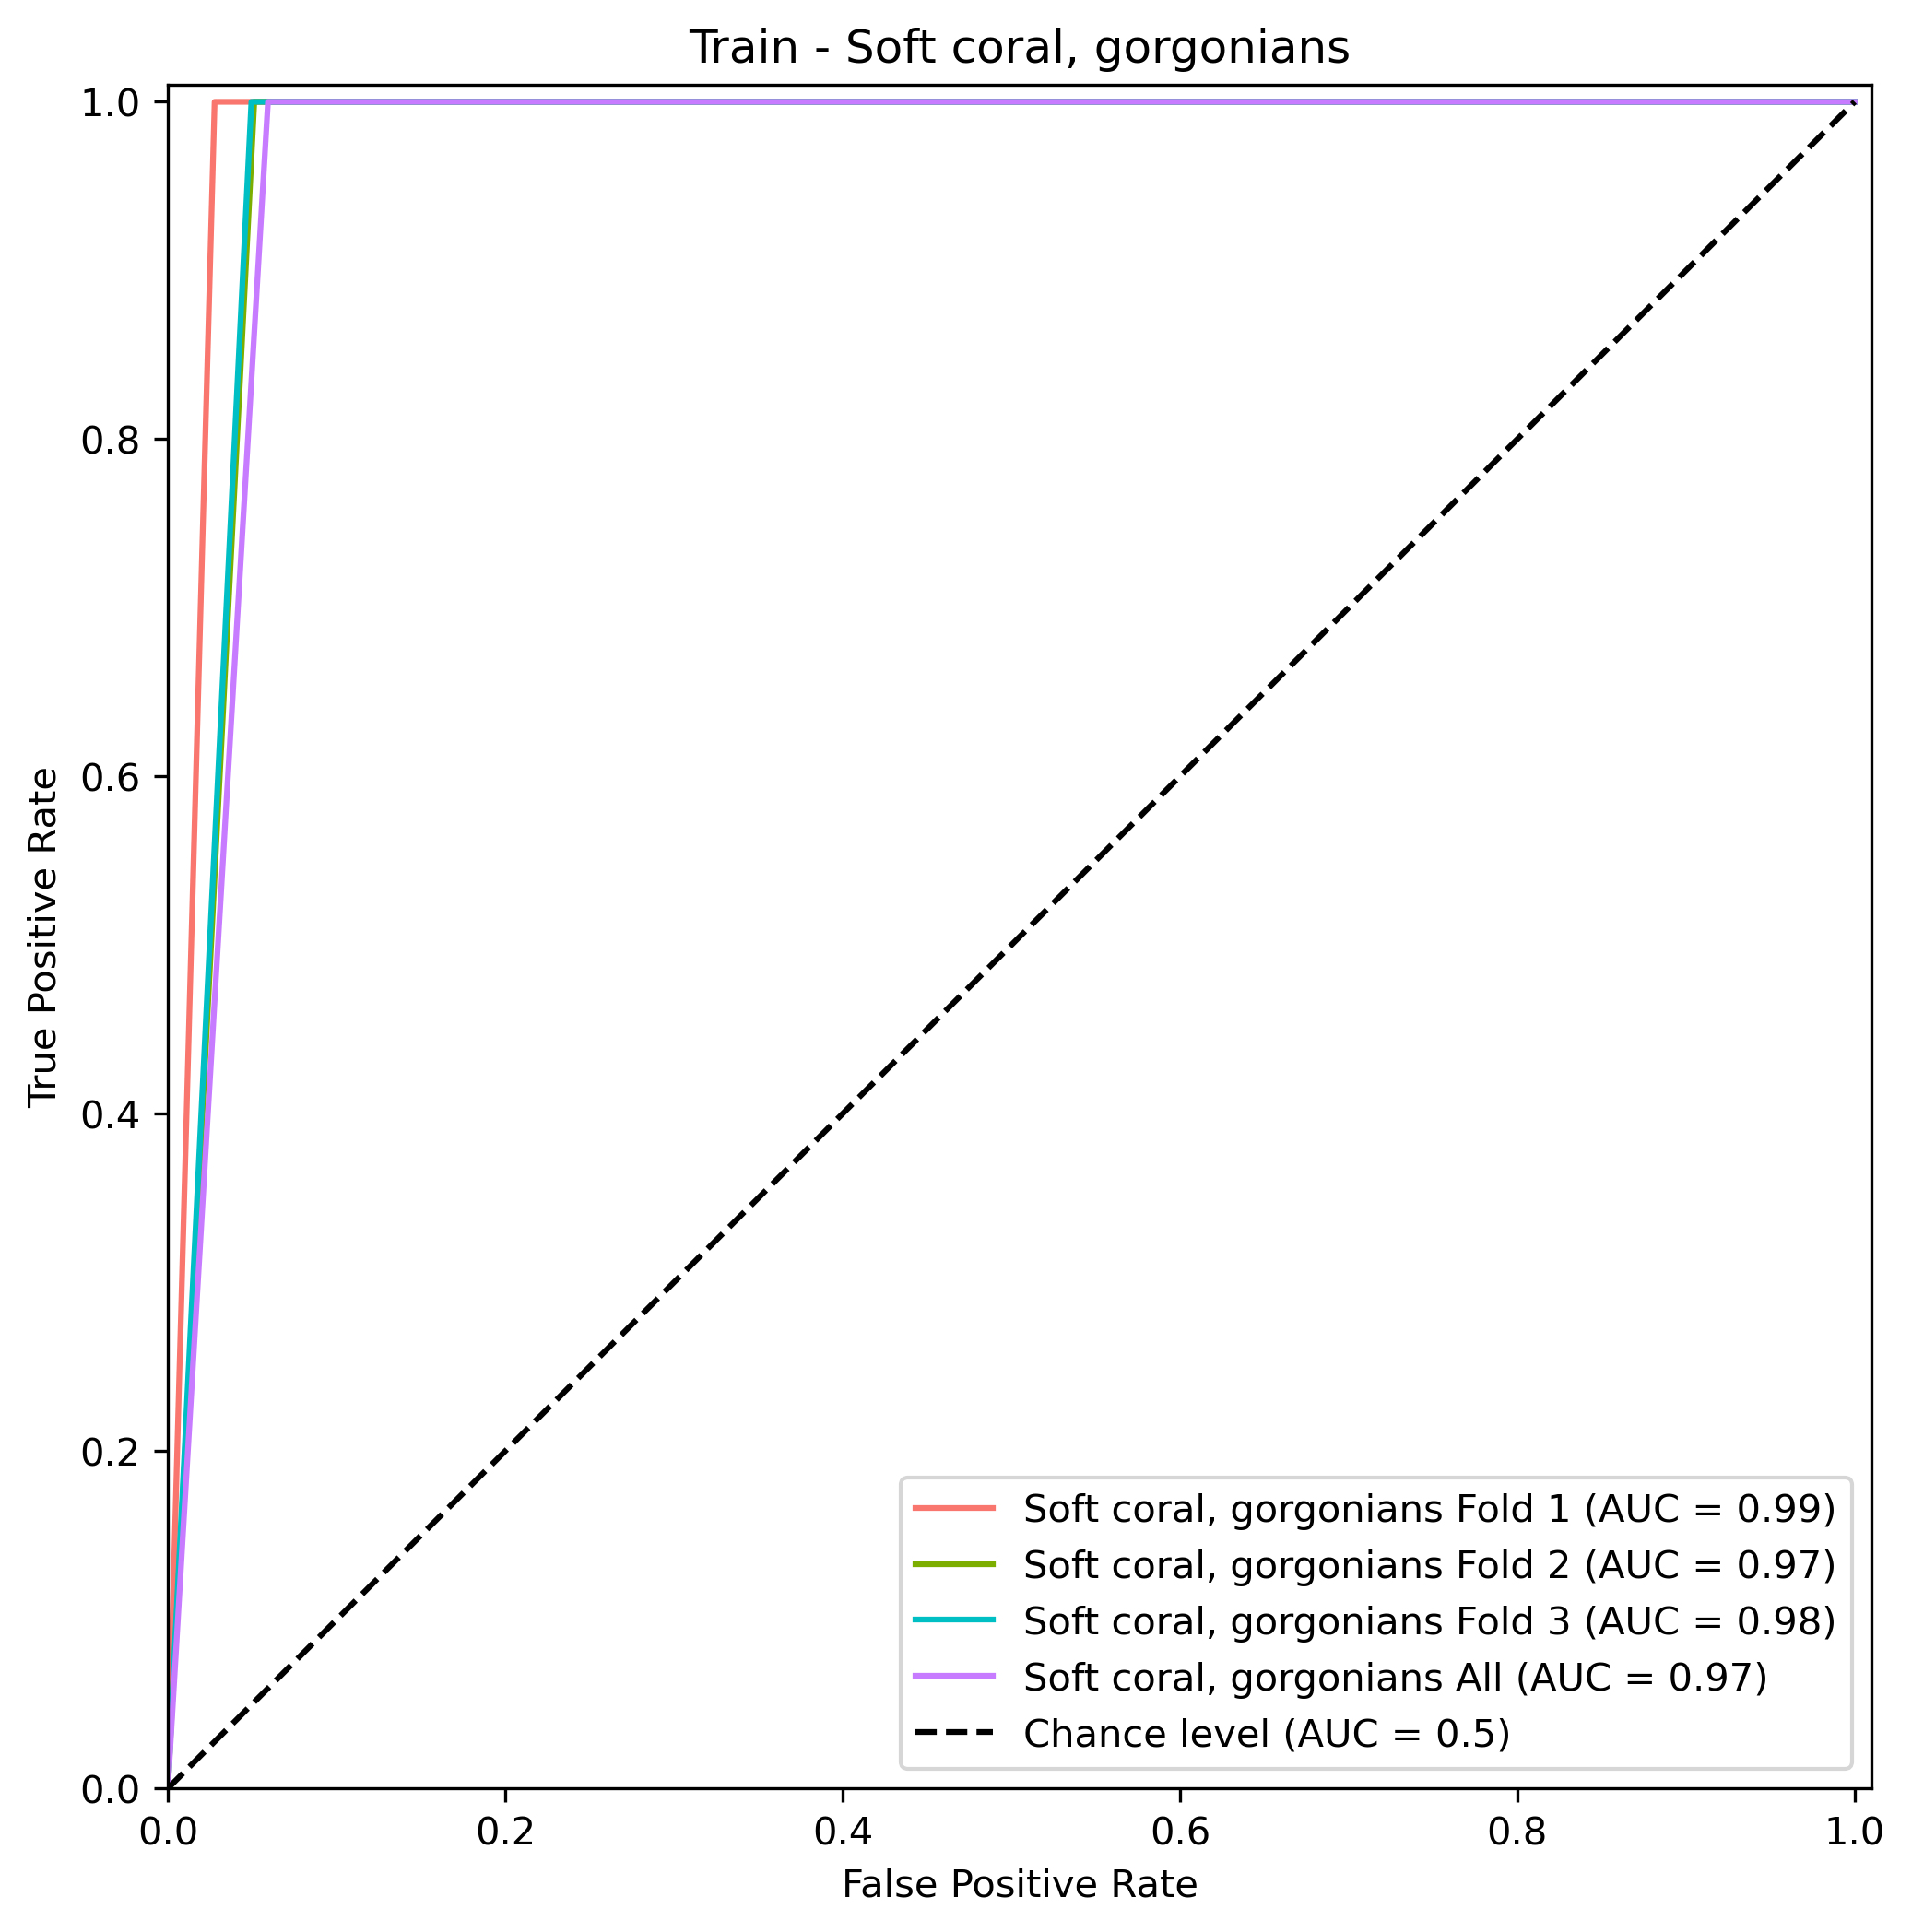
\includegraphics{03-Chapitre3/figures/supplementary/03-receiver_operator_curve_train_rf_Soft coral, gorgonians.png}
\caption{AUC curves of the explanatory power for the Soft coral and
gorgonians.}\label{fig:chap3figS19}
}
\end{figure}

\begin{figure}
\hypertarget{fig:chap3figS20}{%
\centering
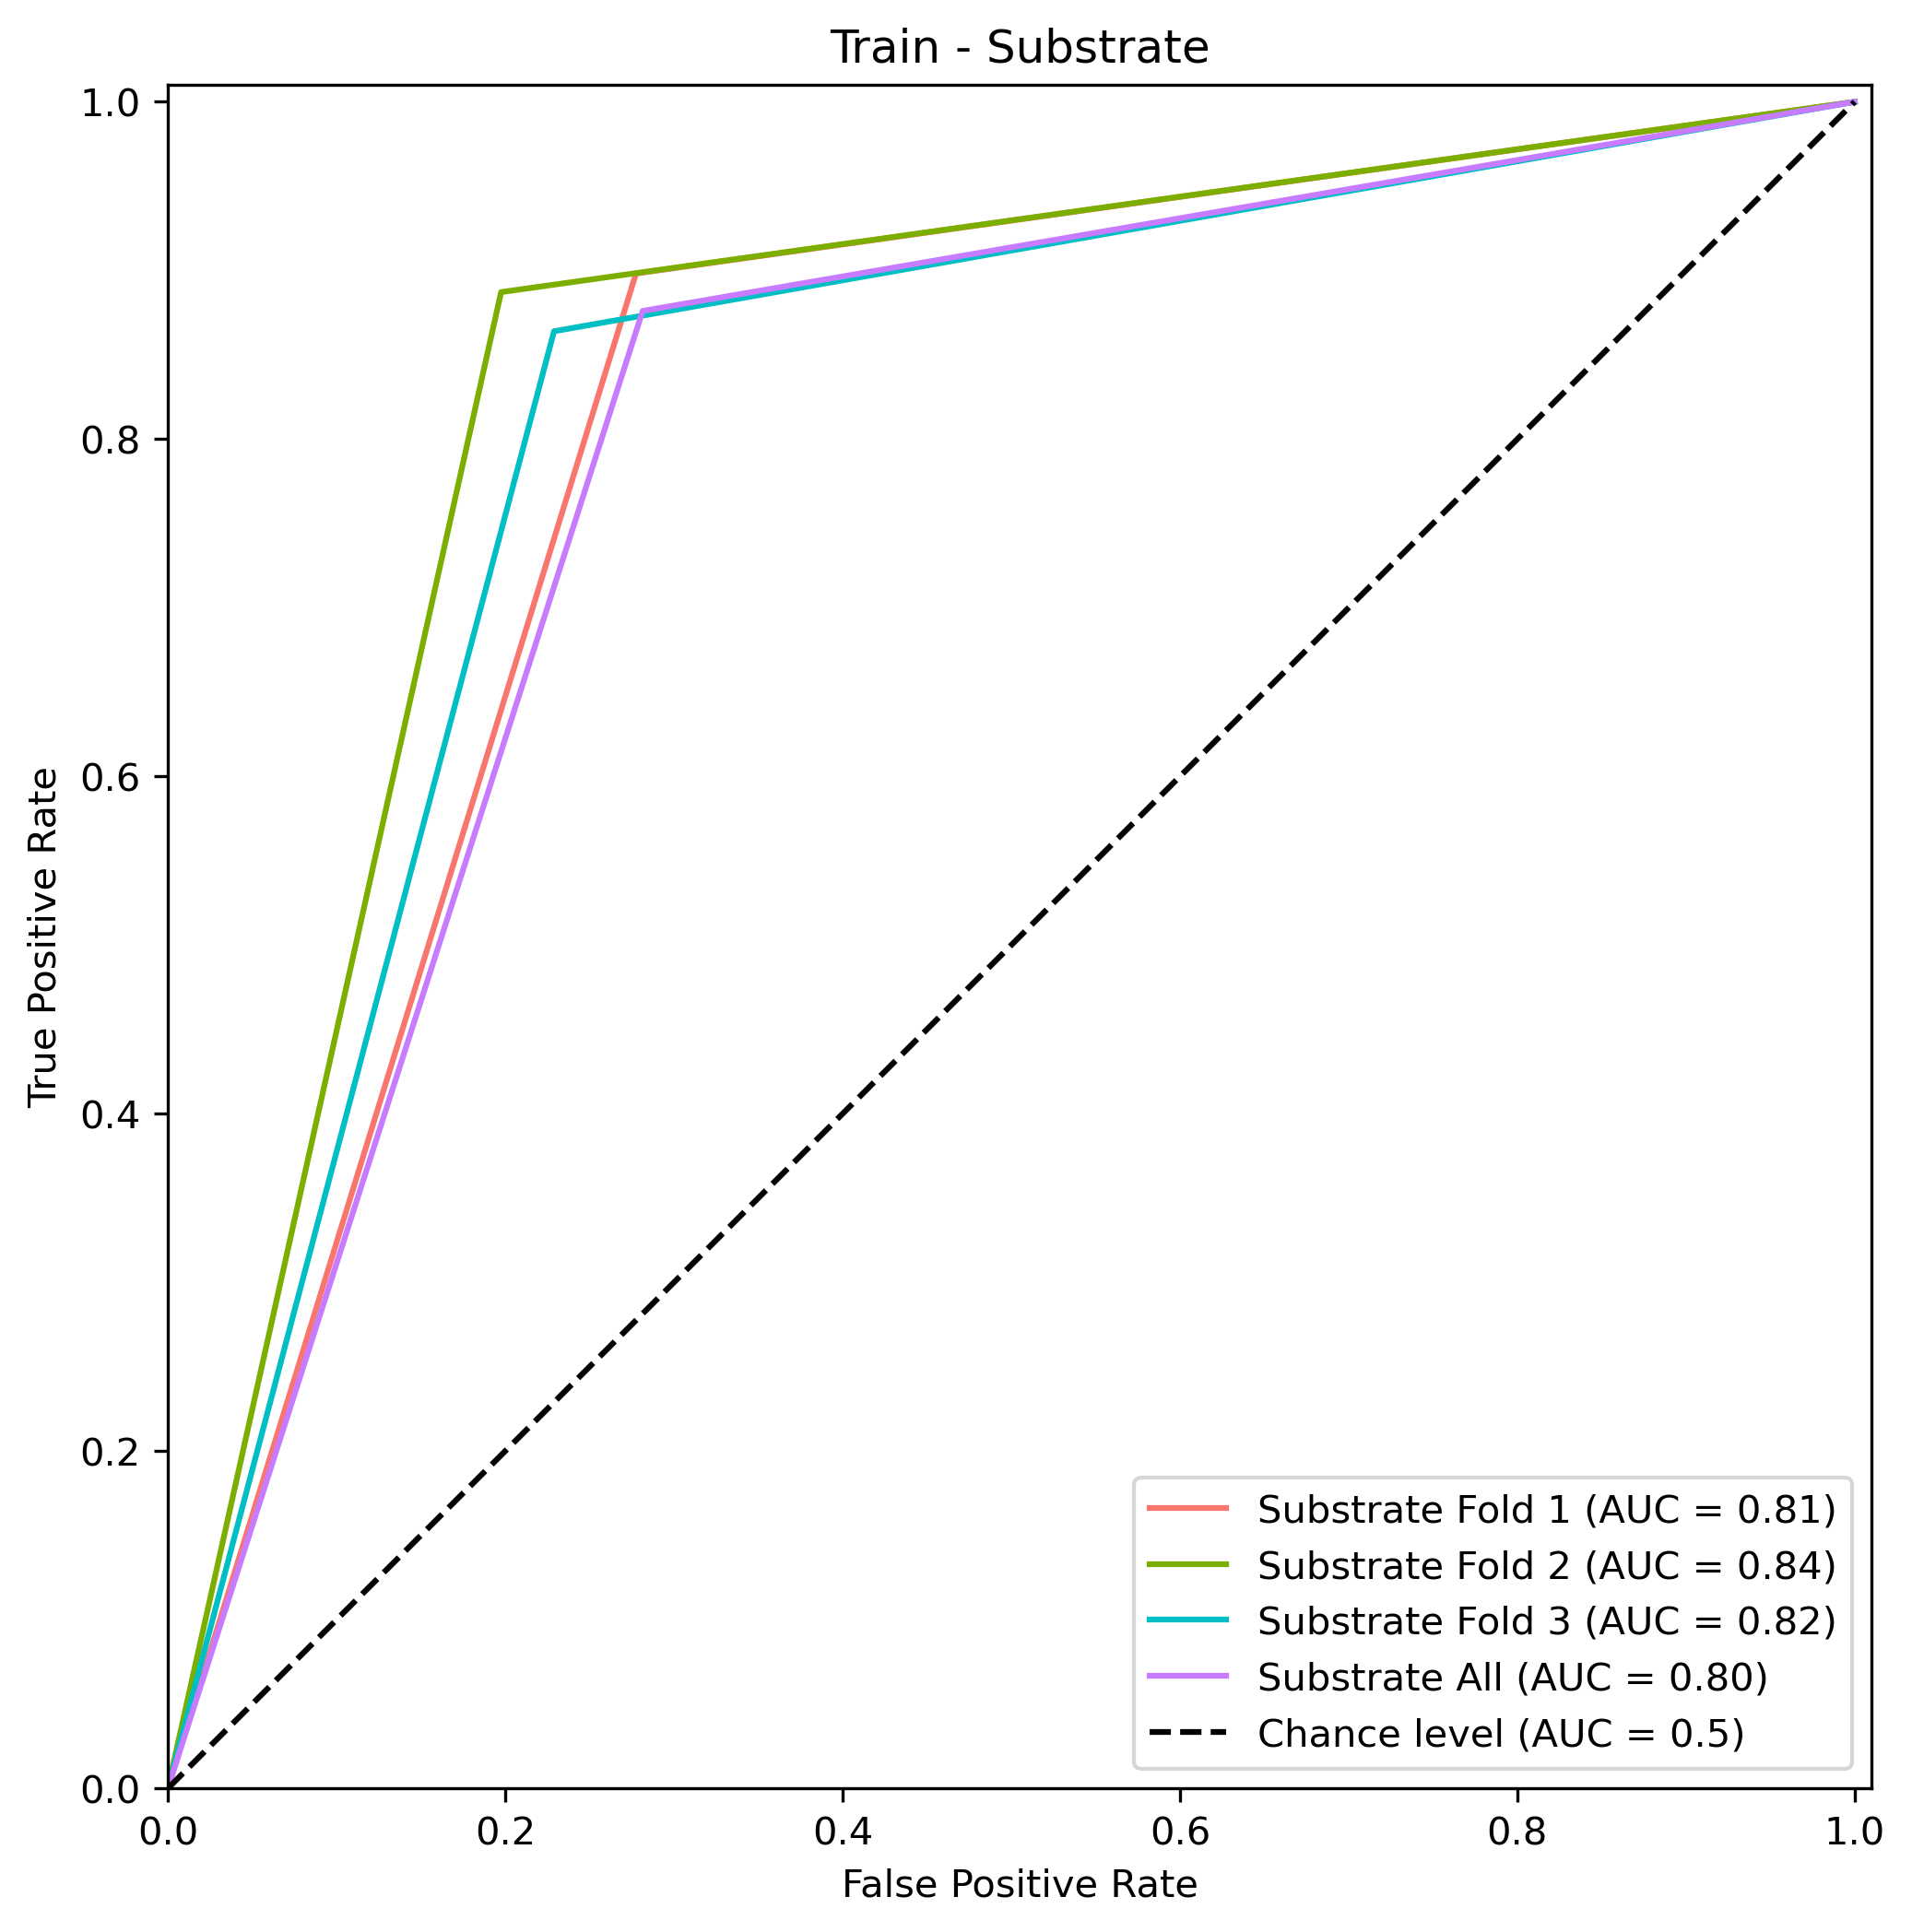
\includegraphics{03-Chapitre3/figures/supplementary/03-receiver_operator_curve_train_rf_Substrate.png}
\caption{AUC curves of the explanatory power for the
Substrate.}\label{fig:chap3figS20}
}
\end{figure}

\begin{figure}
\hypertarget{fig:chap3figS21}{%
\centering
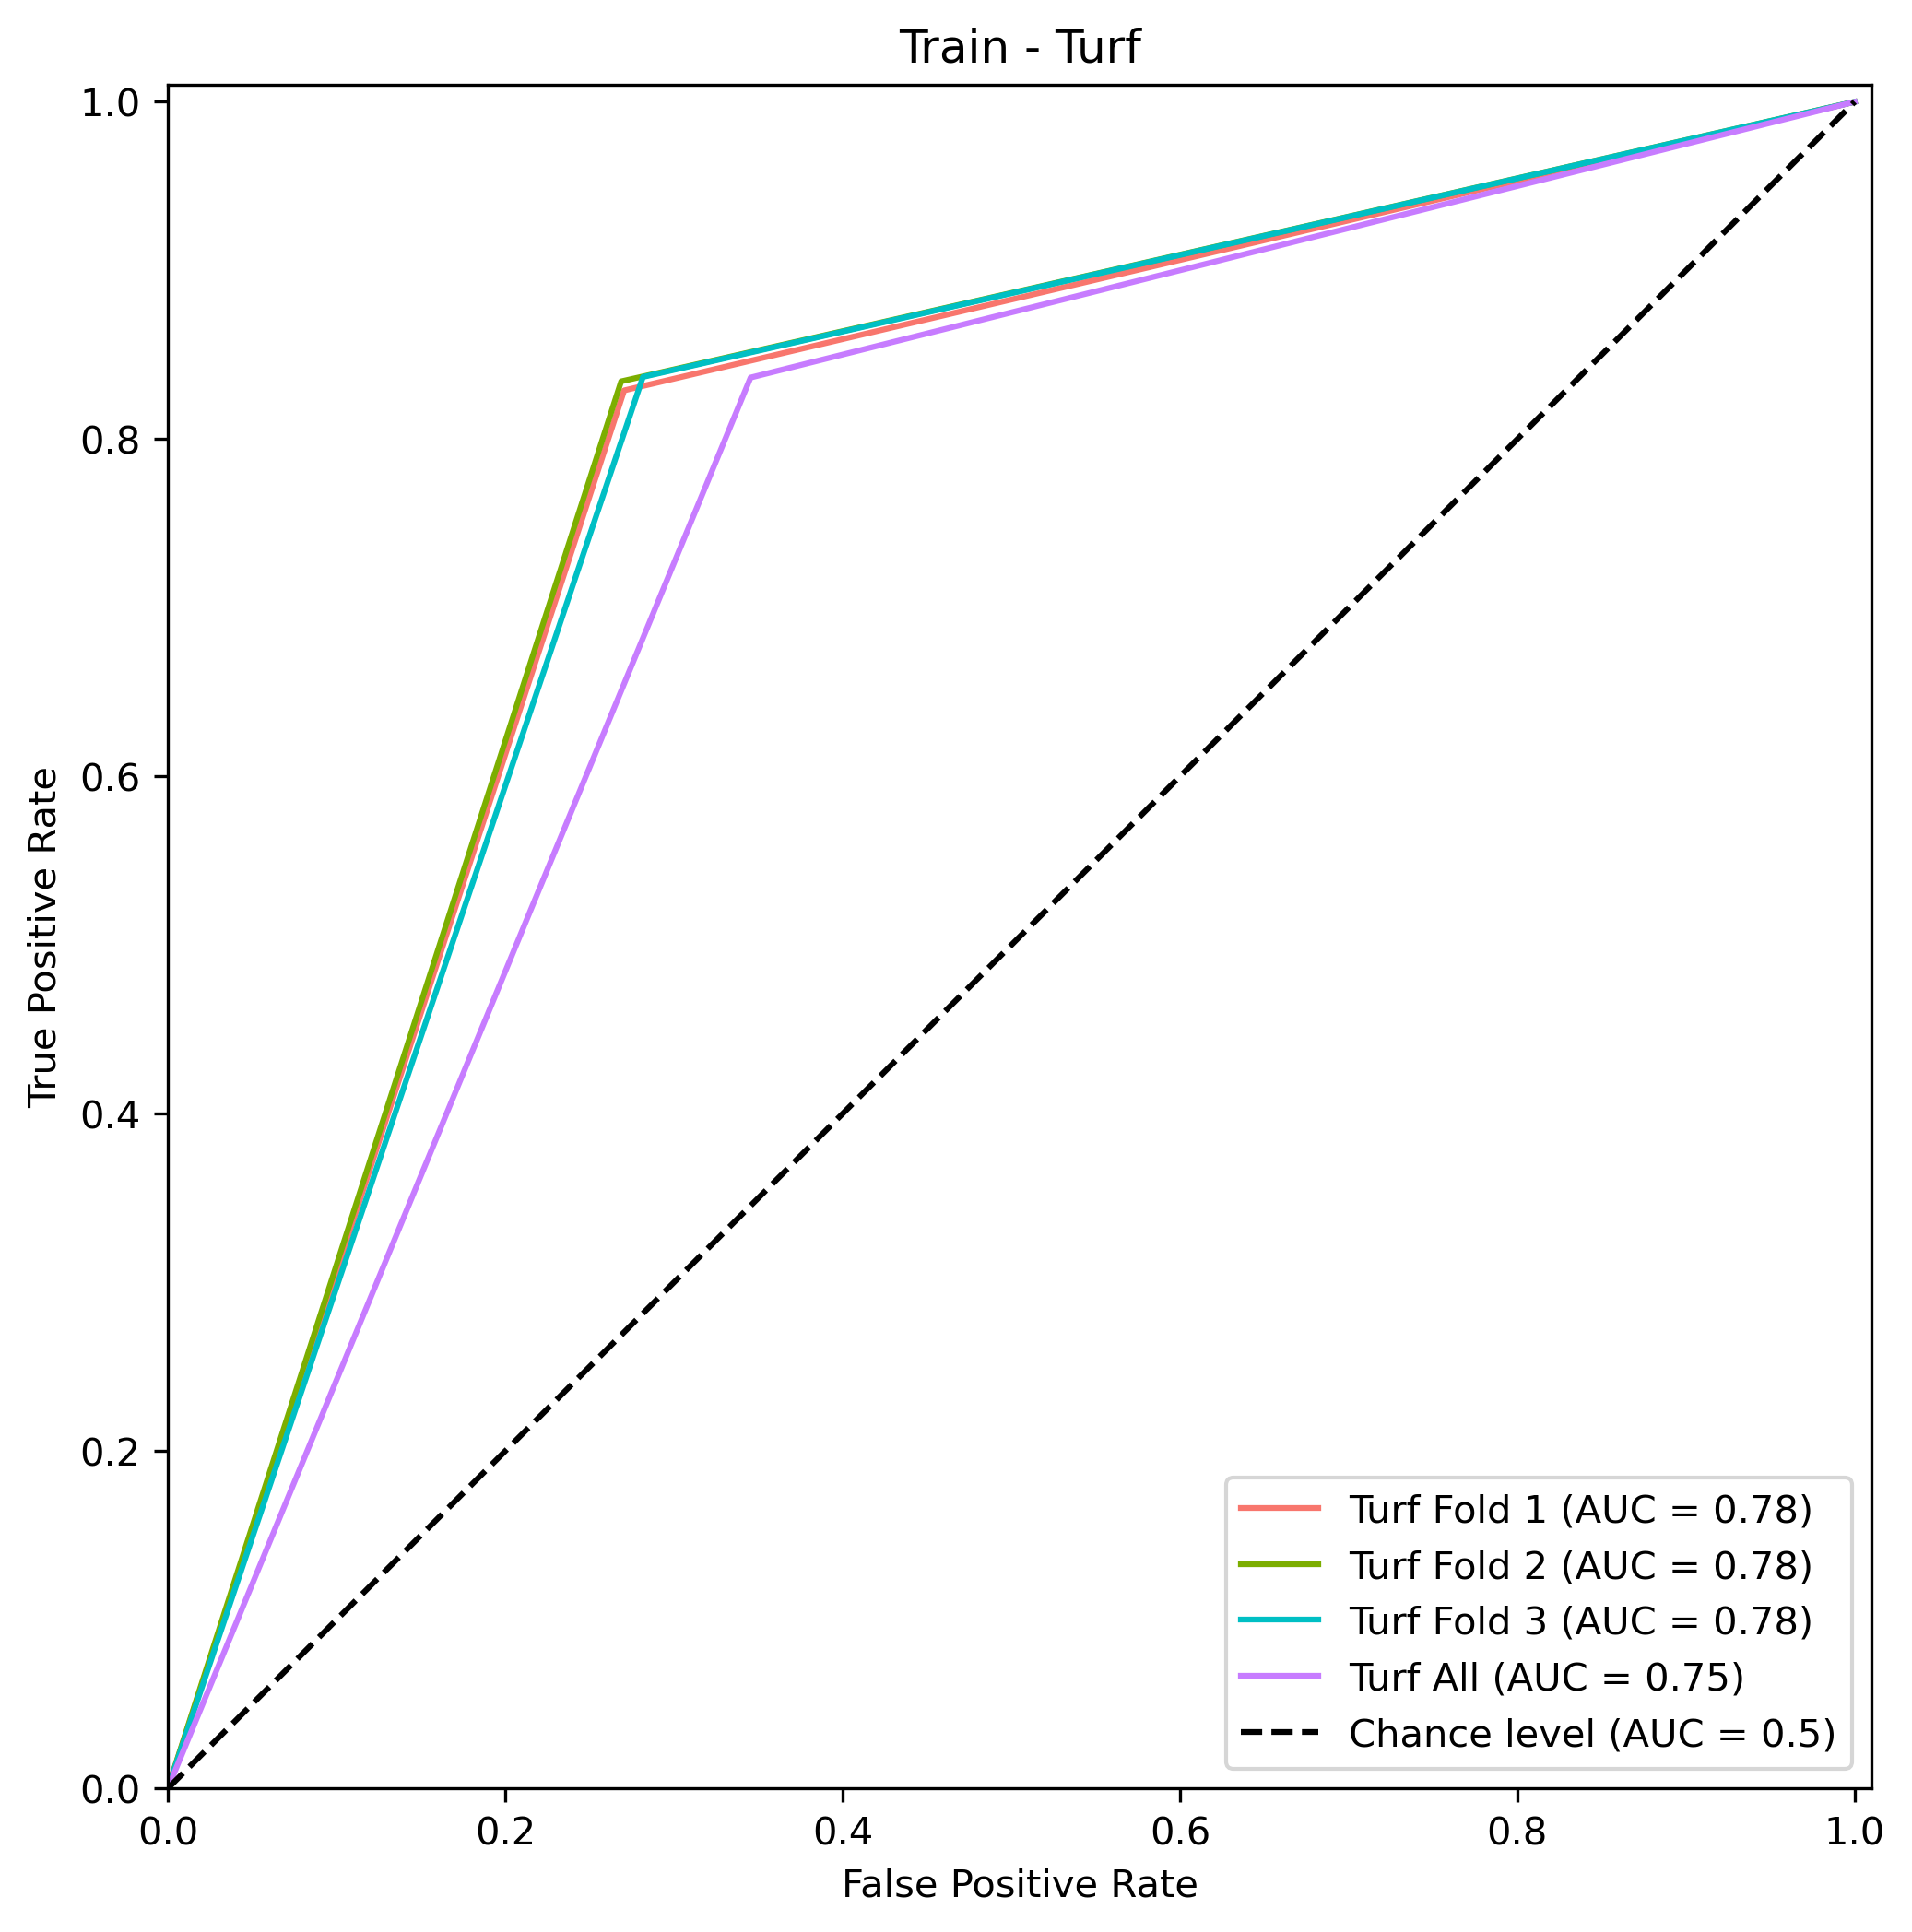
\includegraphics{03-Chapitre3/figures/supplementary/03-receiver_operator_curve_train_rf_Turf.png}
\caption{AUC curves of the explanatory power for the
Turf.}\label{fig:chap3figS21}
}
\end{figure}

\hypertarget{auprc-curves}{%
\subsubsection*{AUPRC Curves}\label{auprc-curves}}

\begin{figure}
\hypertarget{fig:chap3figS22}{%
\centering
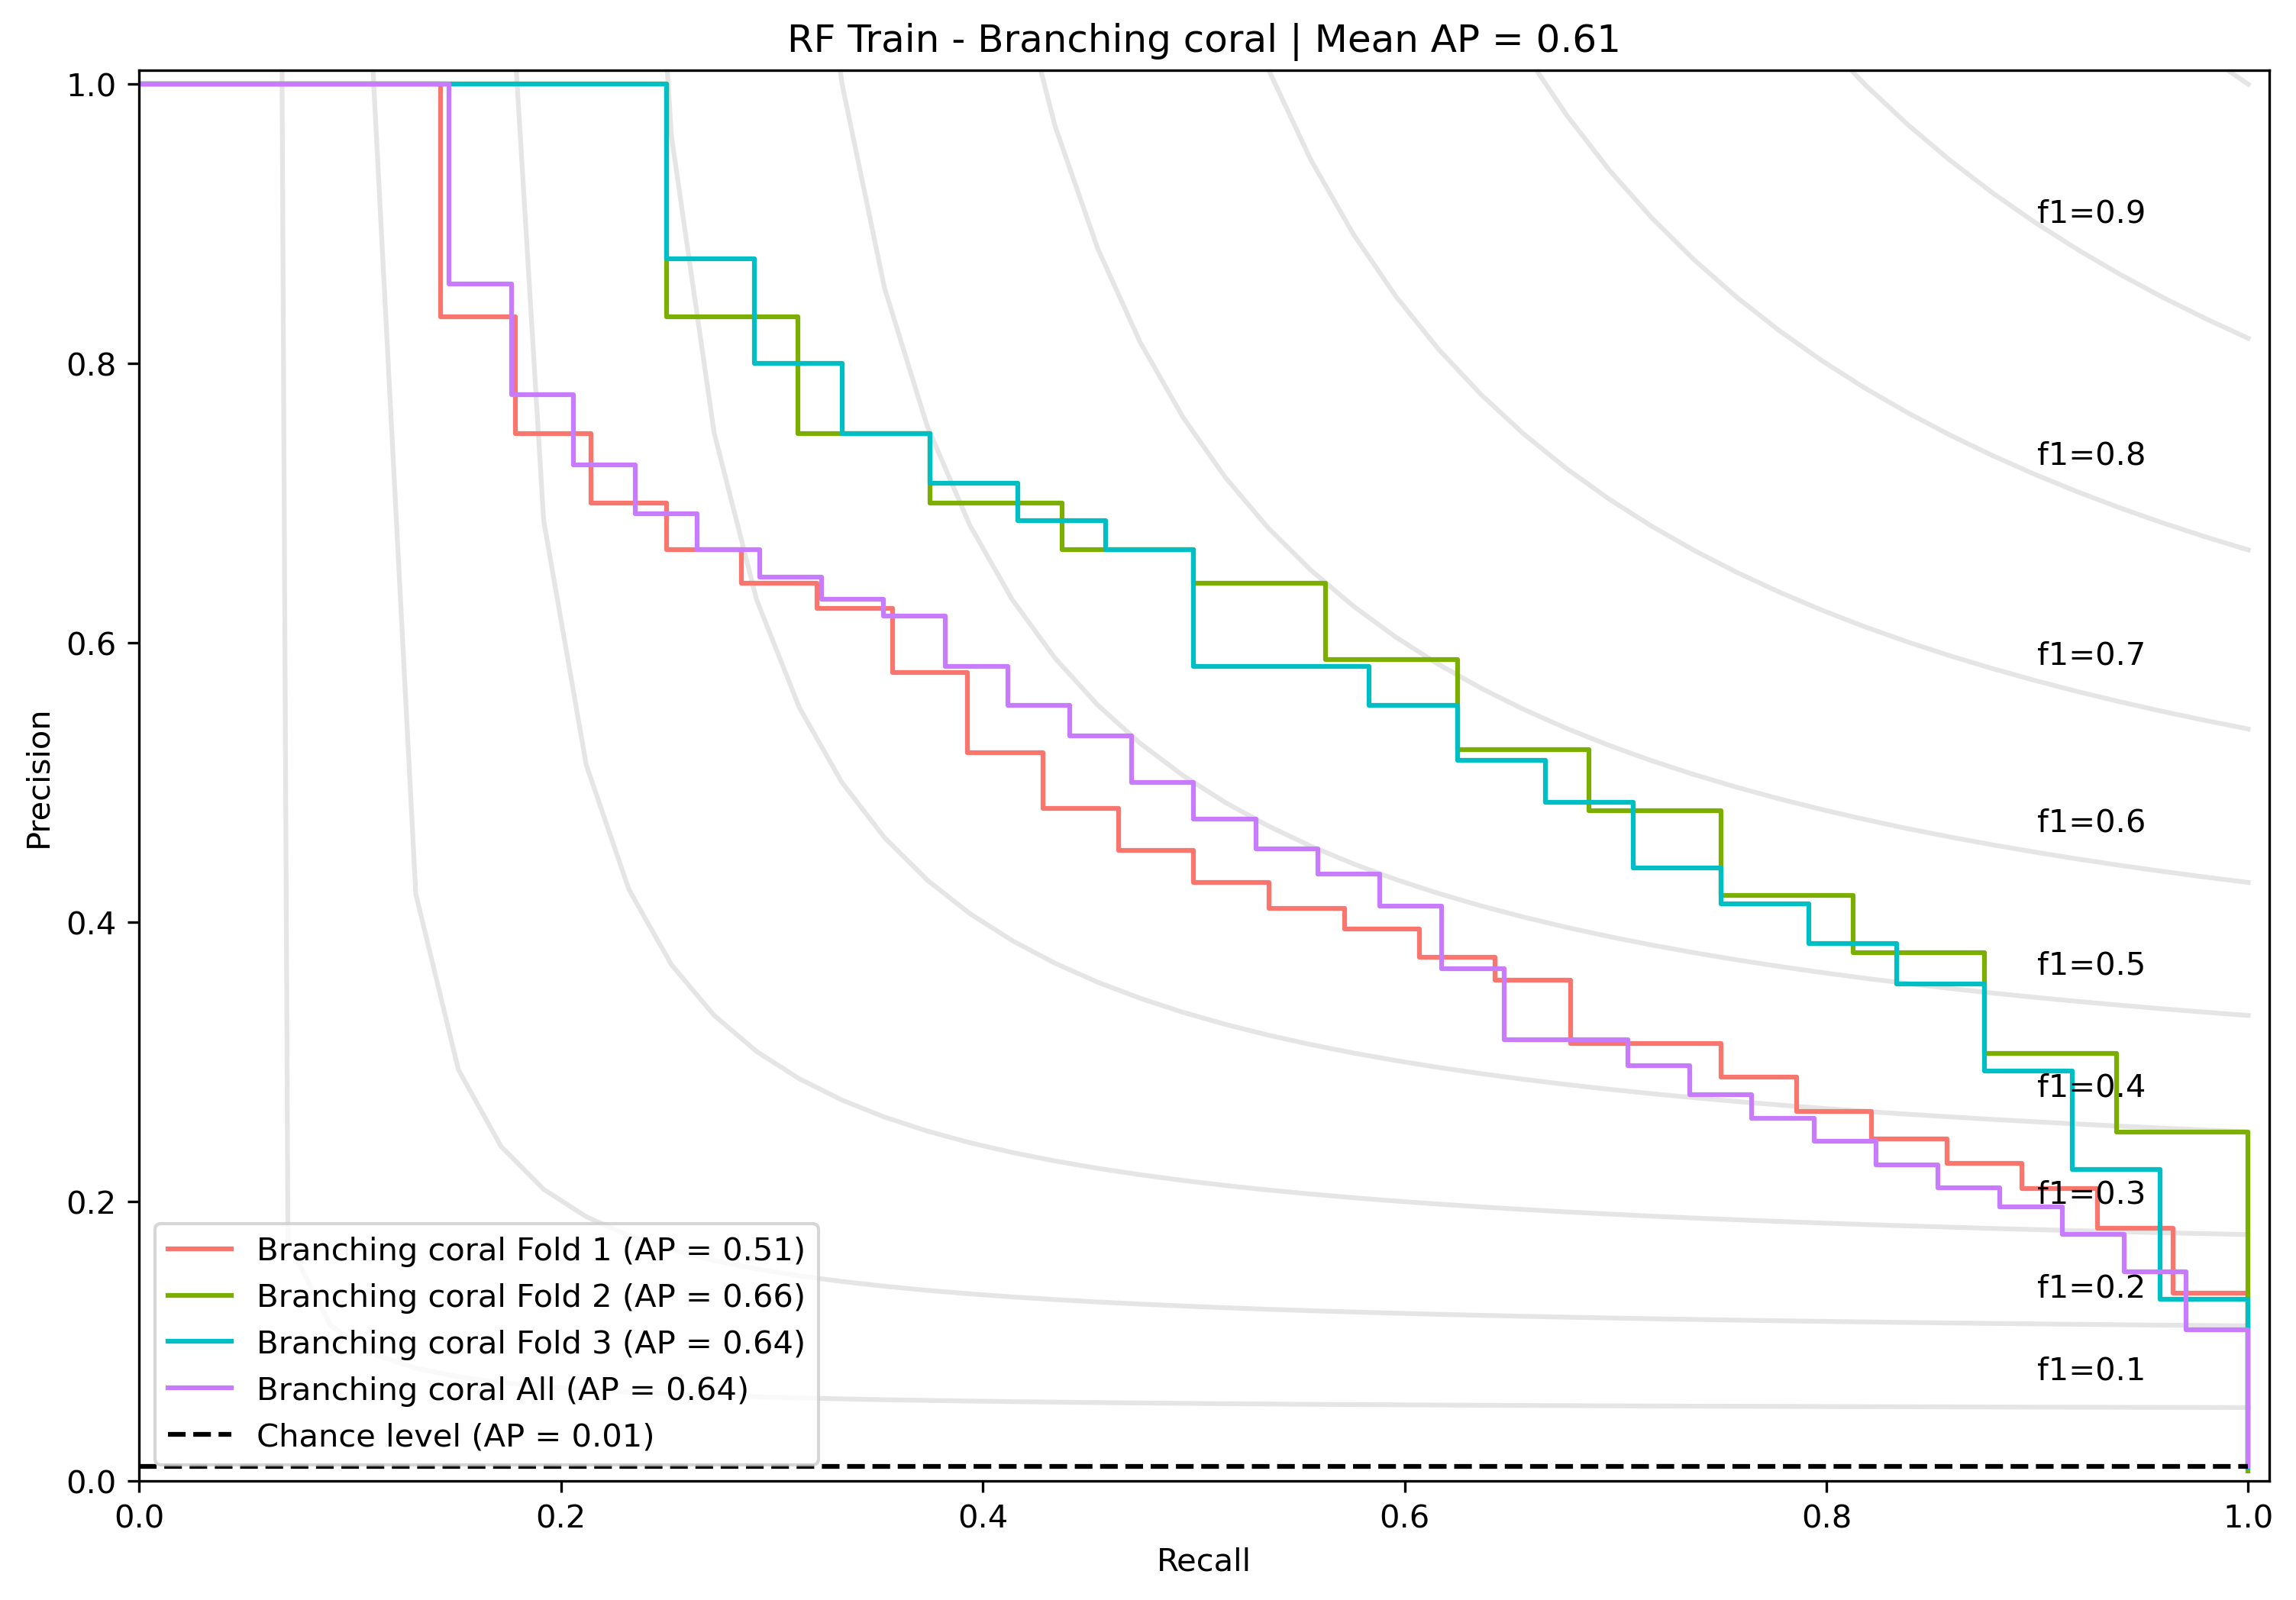
\includegraphics{03-Chapitre3/figures/supplementary/03-precision_recall_curve_train_rf_Branching coral.png}
\caption{AUPRC curves of the explanatory power for the Branching coral.
The grey lines represent isolines of F1-score.}\label{fig:chap3figS22}
}
\end{figure}

\begin{figure}
\hypertarget{fig:chap3figS23}{%
\centering
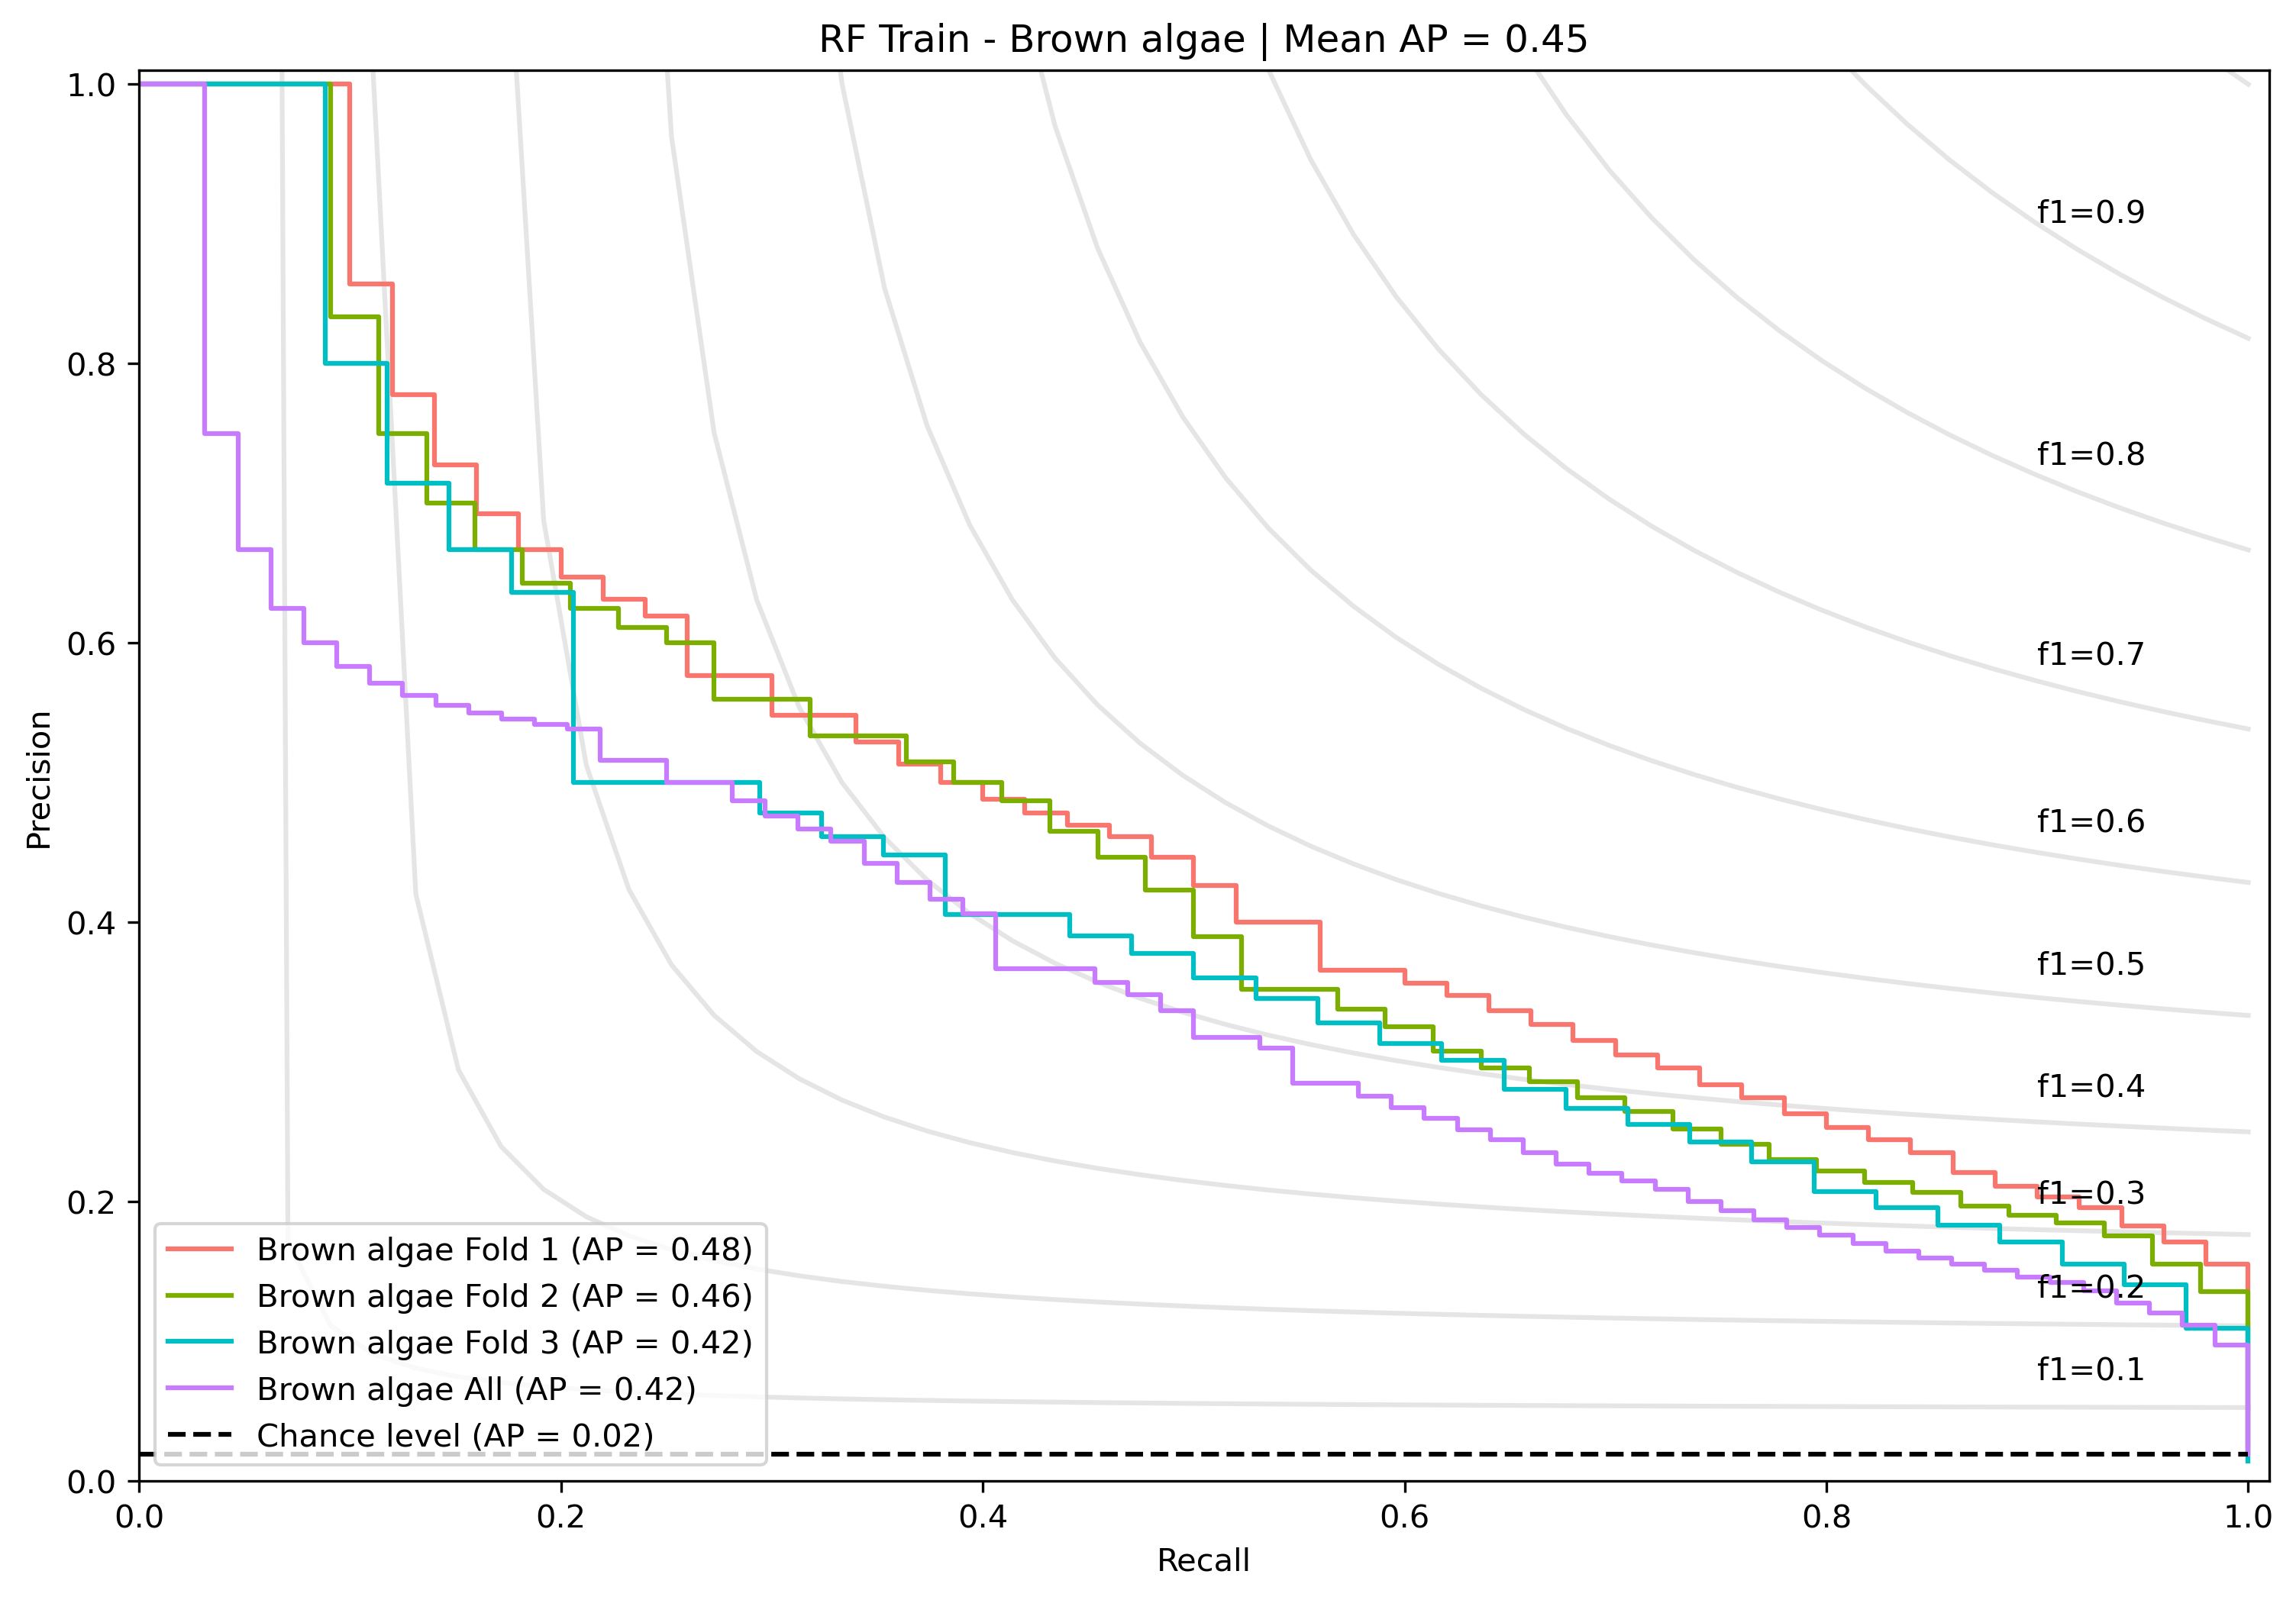
\includegraphics{03-Chapitre3/figures/supplementary/03-precision_recall_curve_train_rf_Brown algae.png}
\caption{AUPRC curves of the explanatory power for the Brown algae. The
grey lines represent isolines of F1-score.}\label{fig:chap3figS23}
}
\end{figure}

\begin{figure}
\hypertarget{fig:chap3figS24}{%
\centering
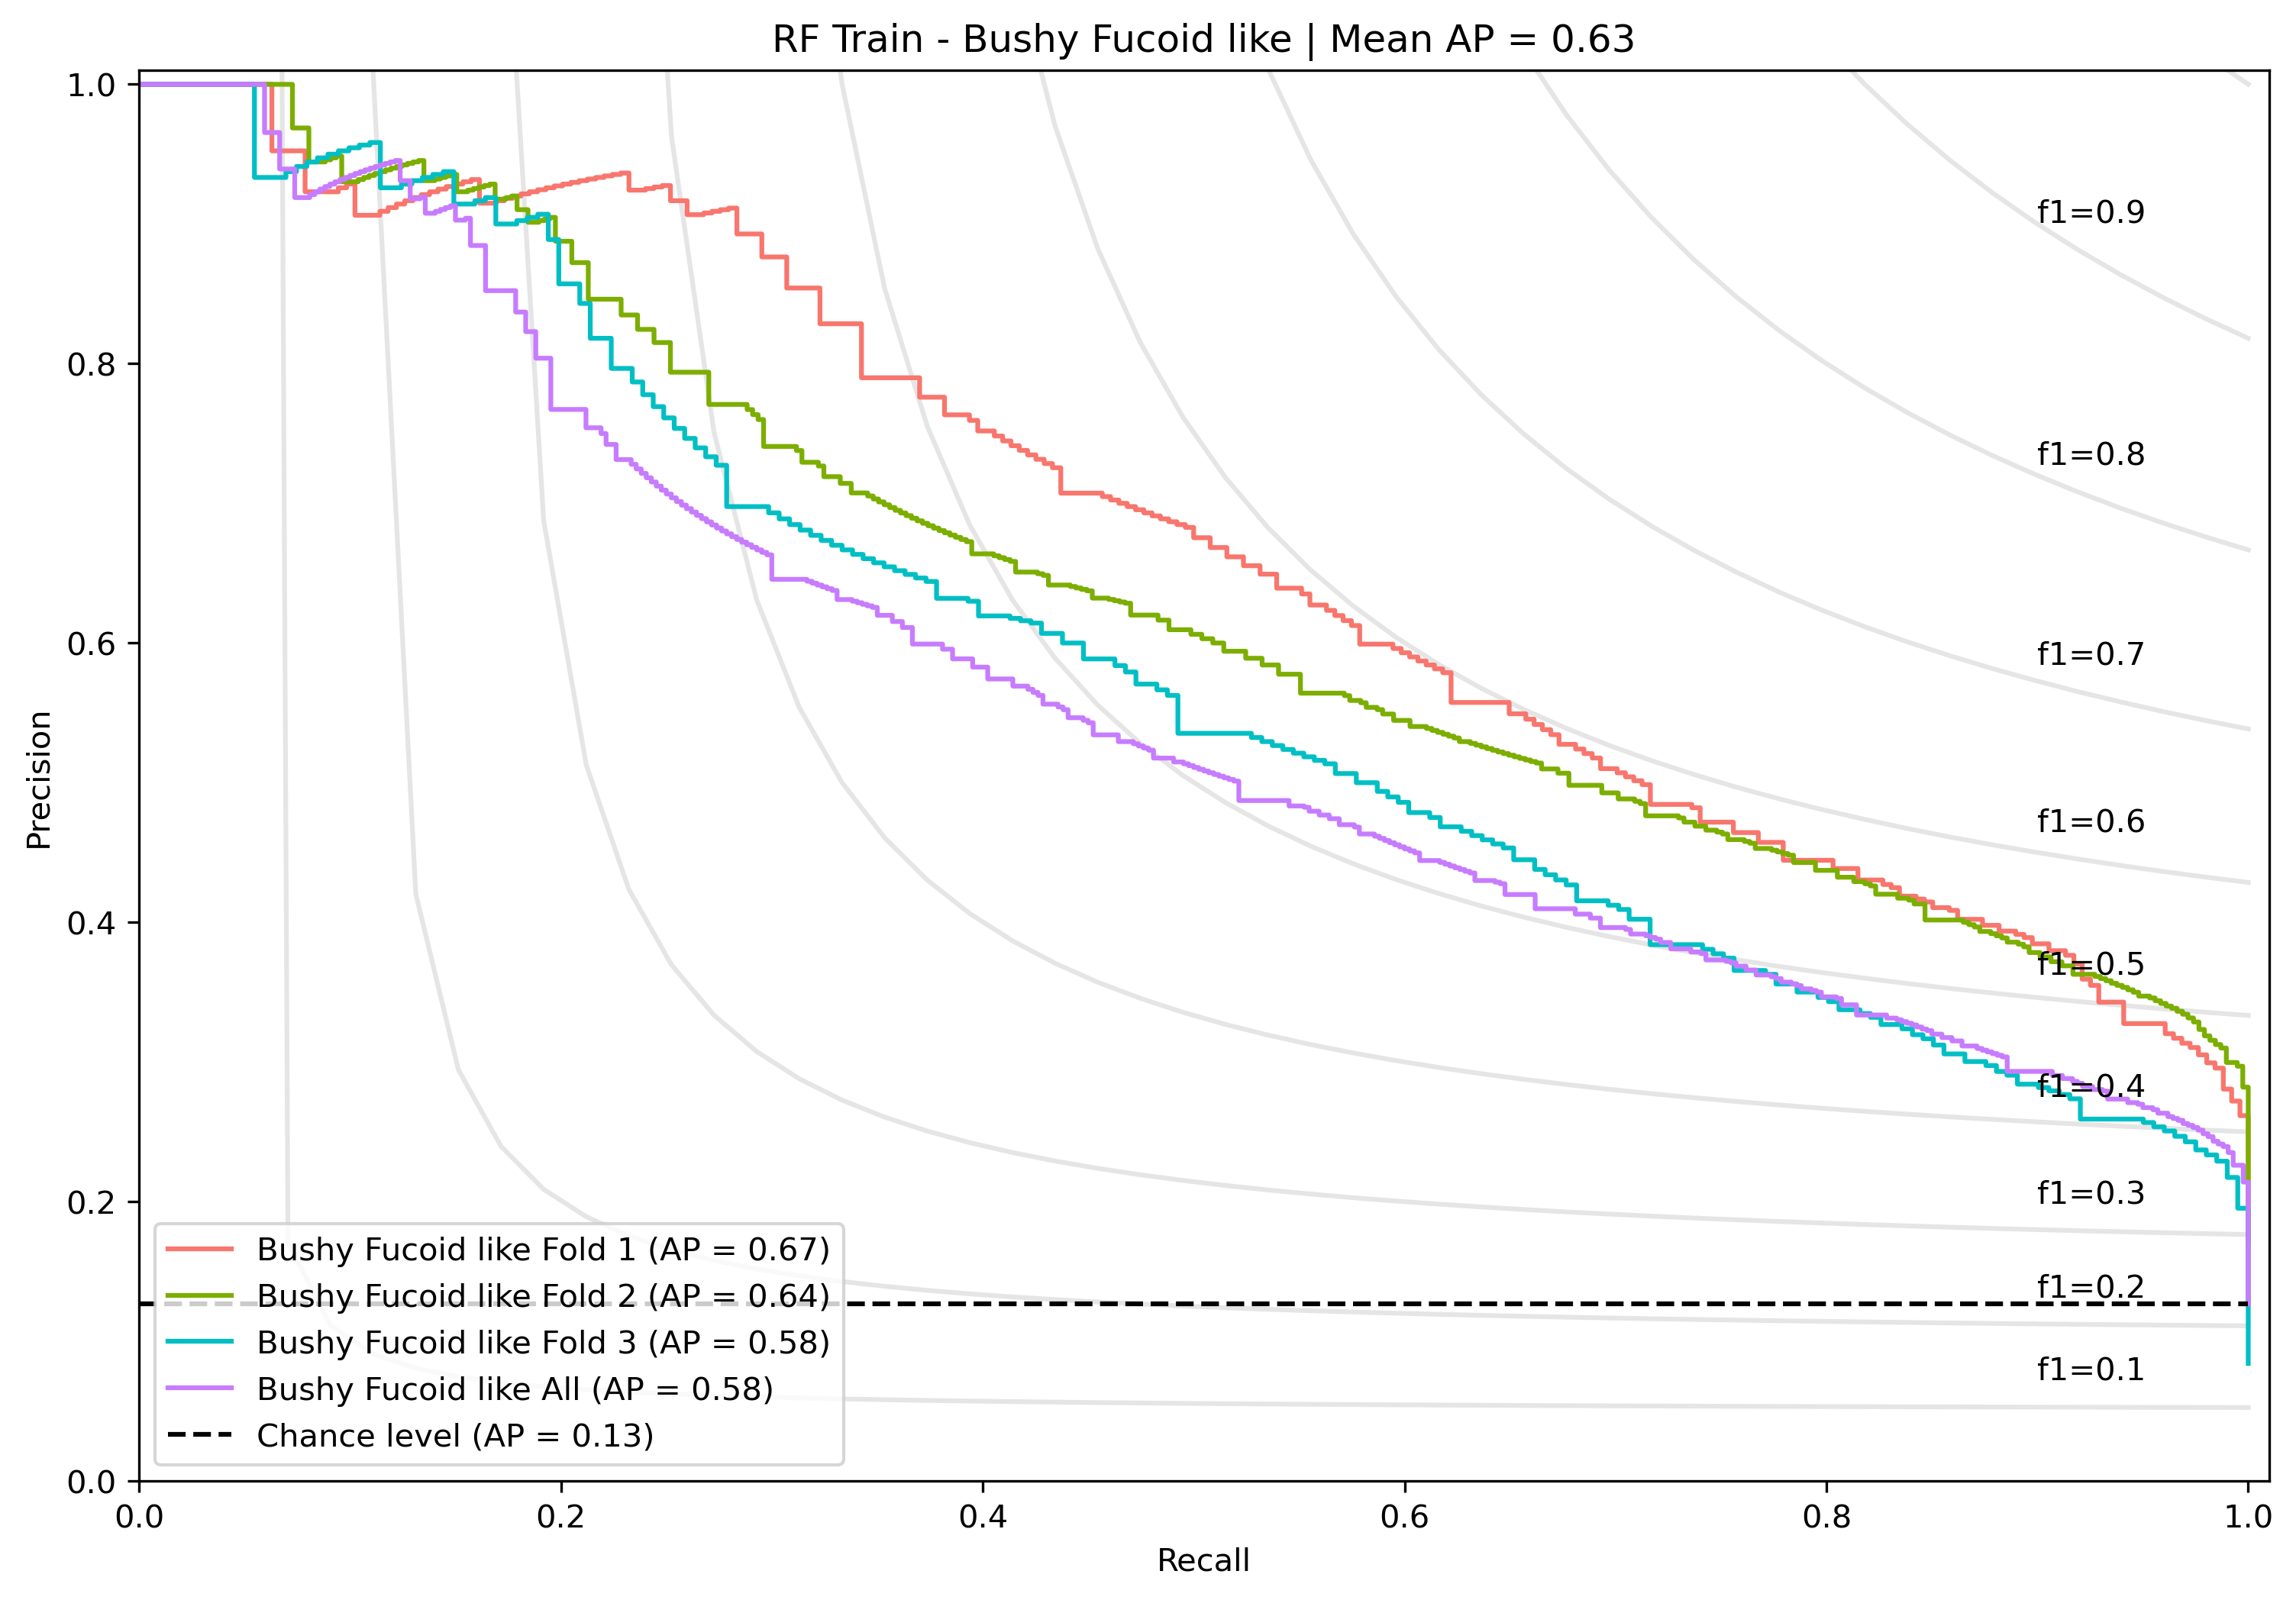
\includegraphics{03-Chapitre3/figures/supplementary/03-precision_recall_curve_train_rf_Bushy Fucoid like.png}
\caption{AUPRC curves of the explanatory power for the Bushy Fucoid
like. The grey lines represent isolines of
F1-score.}\label{fig:chap3figS24}
}
\end{figure}

\begin{figure}
\hypertarget{fig:chap3figS25}{%
\centering
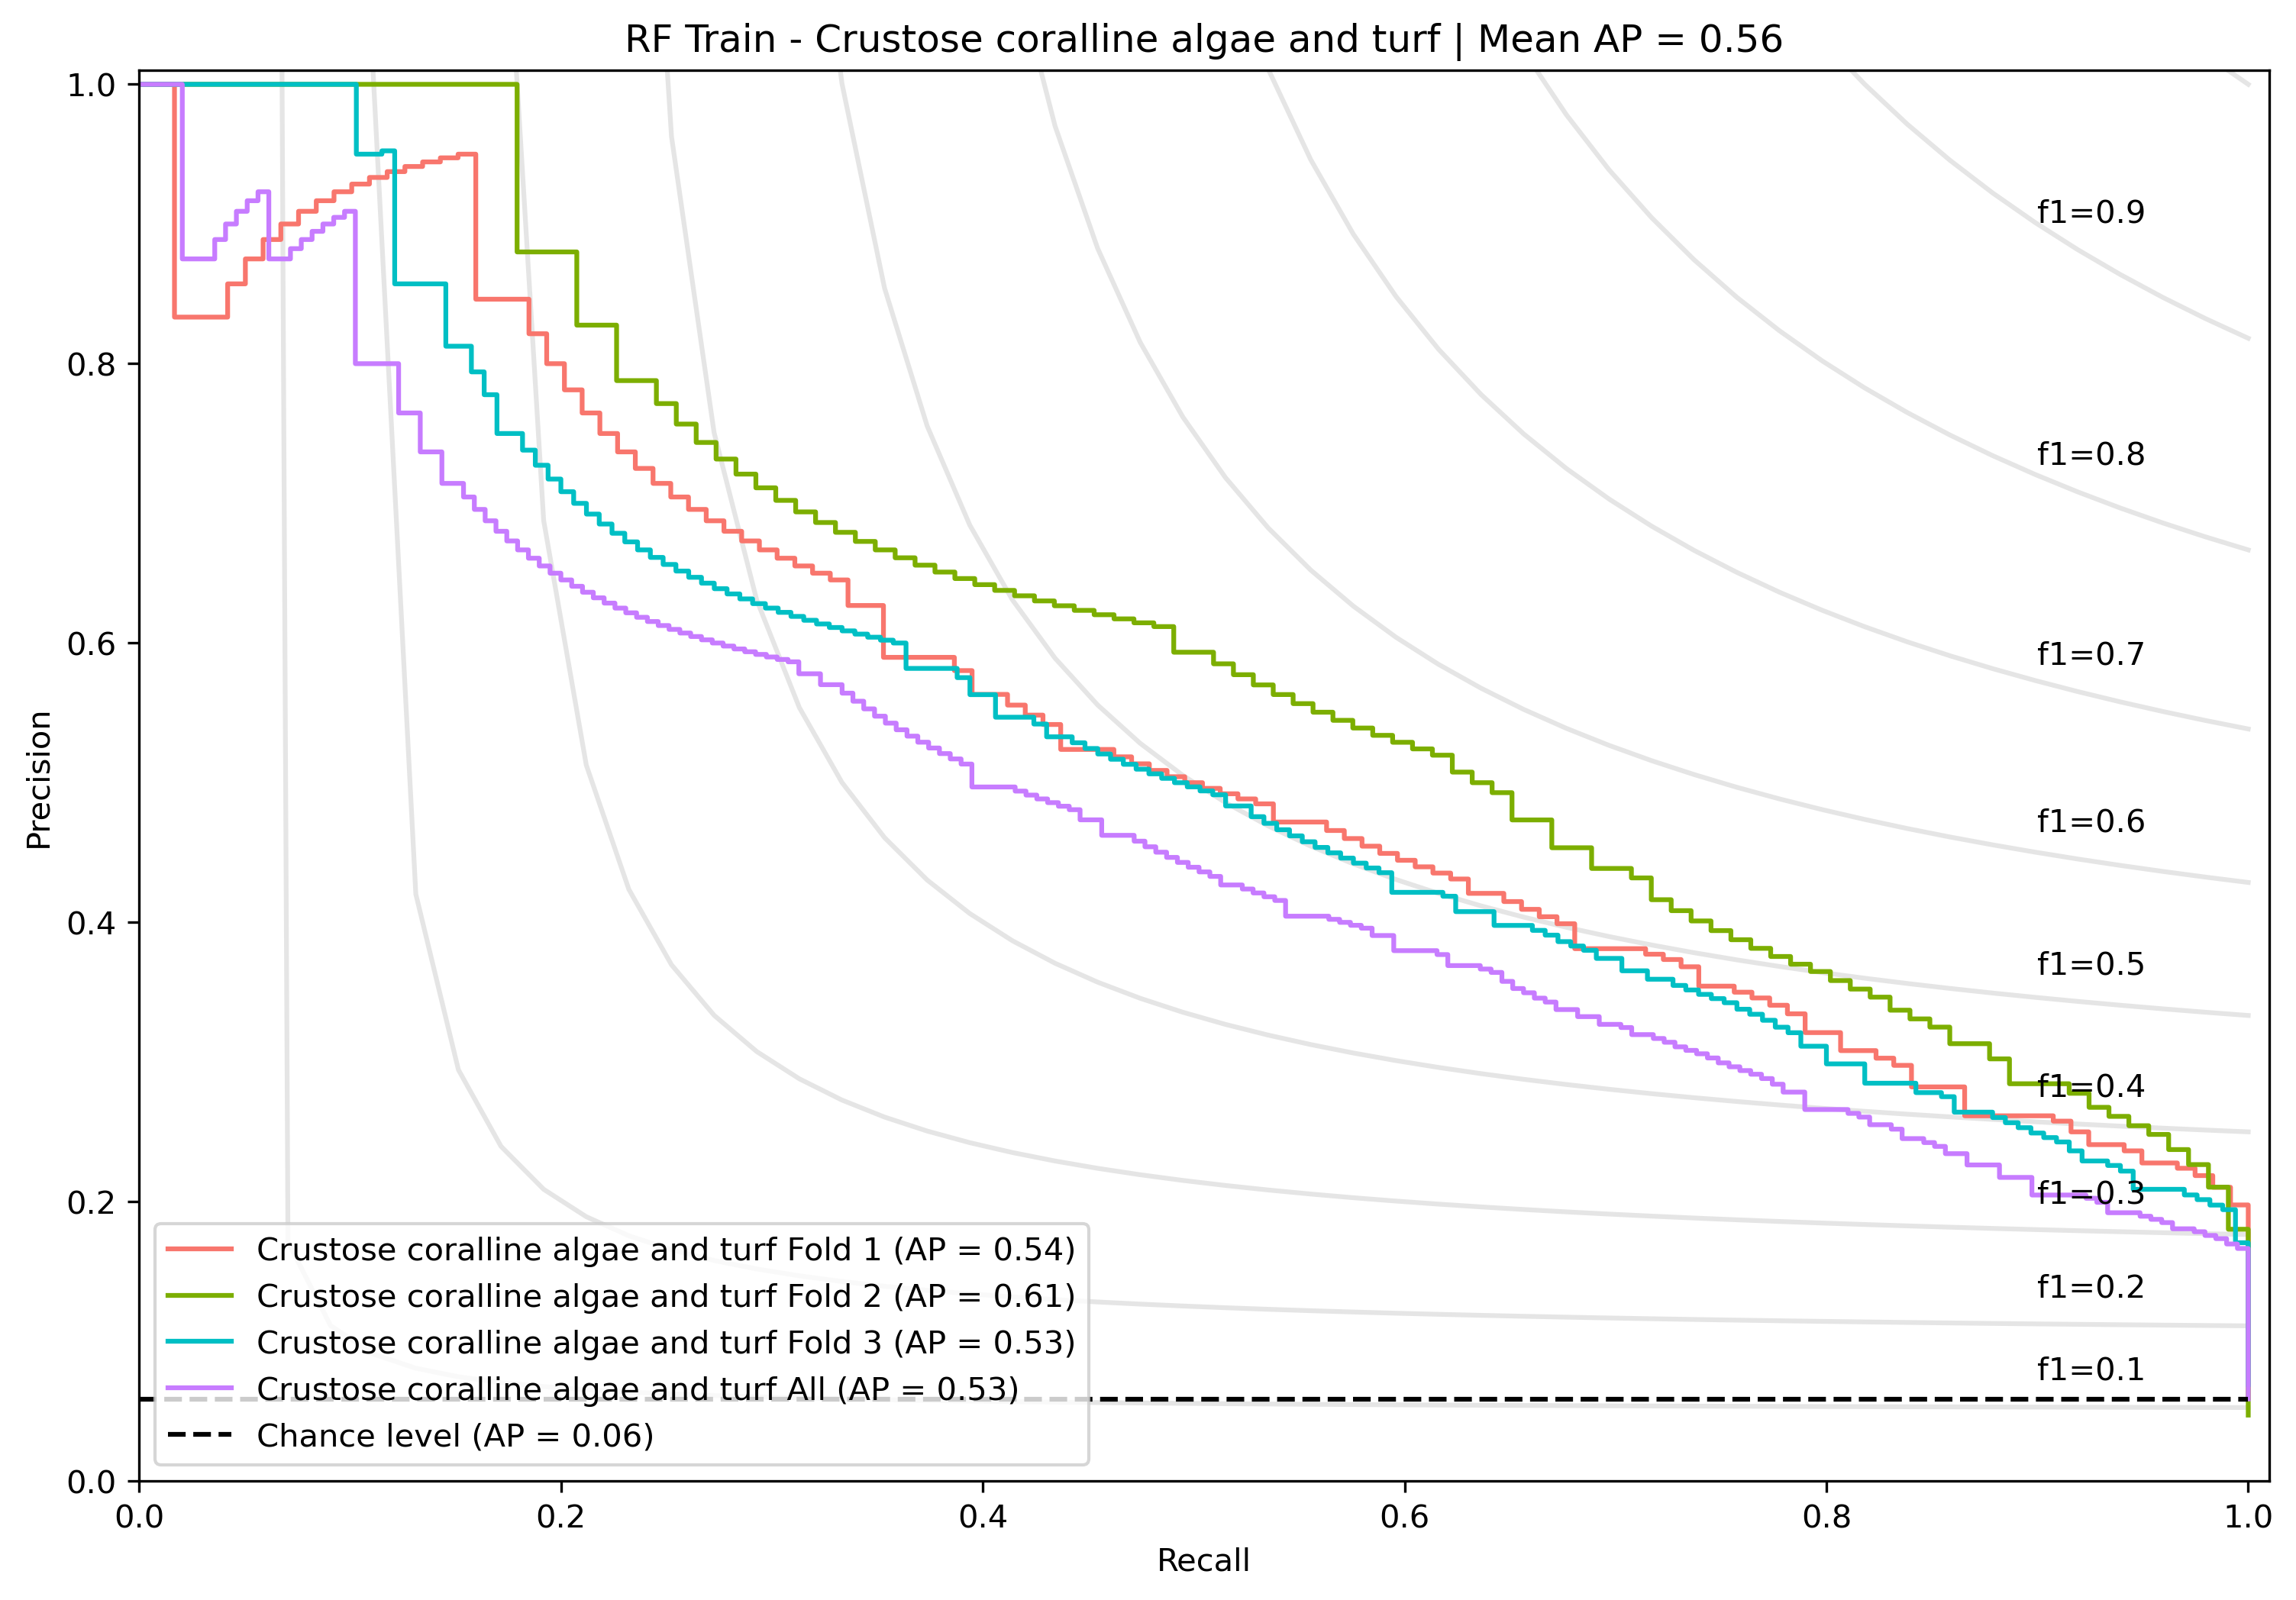
\includegraphics{03-Chapitre3/figures/supplementary/03-precision_recall_curve_train_rf_Crustose coralline algae and turf.png}
\caption{AUPRC curves of the explanatory power for the Crustose
coralline algae and turf. The grey lines represent isolines of
F1-score.}\label{fig:chap3figS25}
}
\end{figure}

\begin{figure}
\hypertarget{fig:chap3figS26}{%
\centering
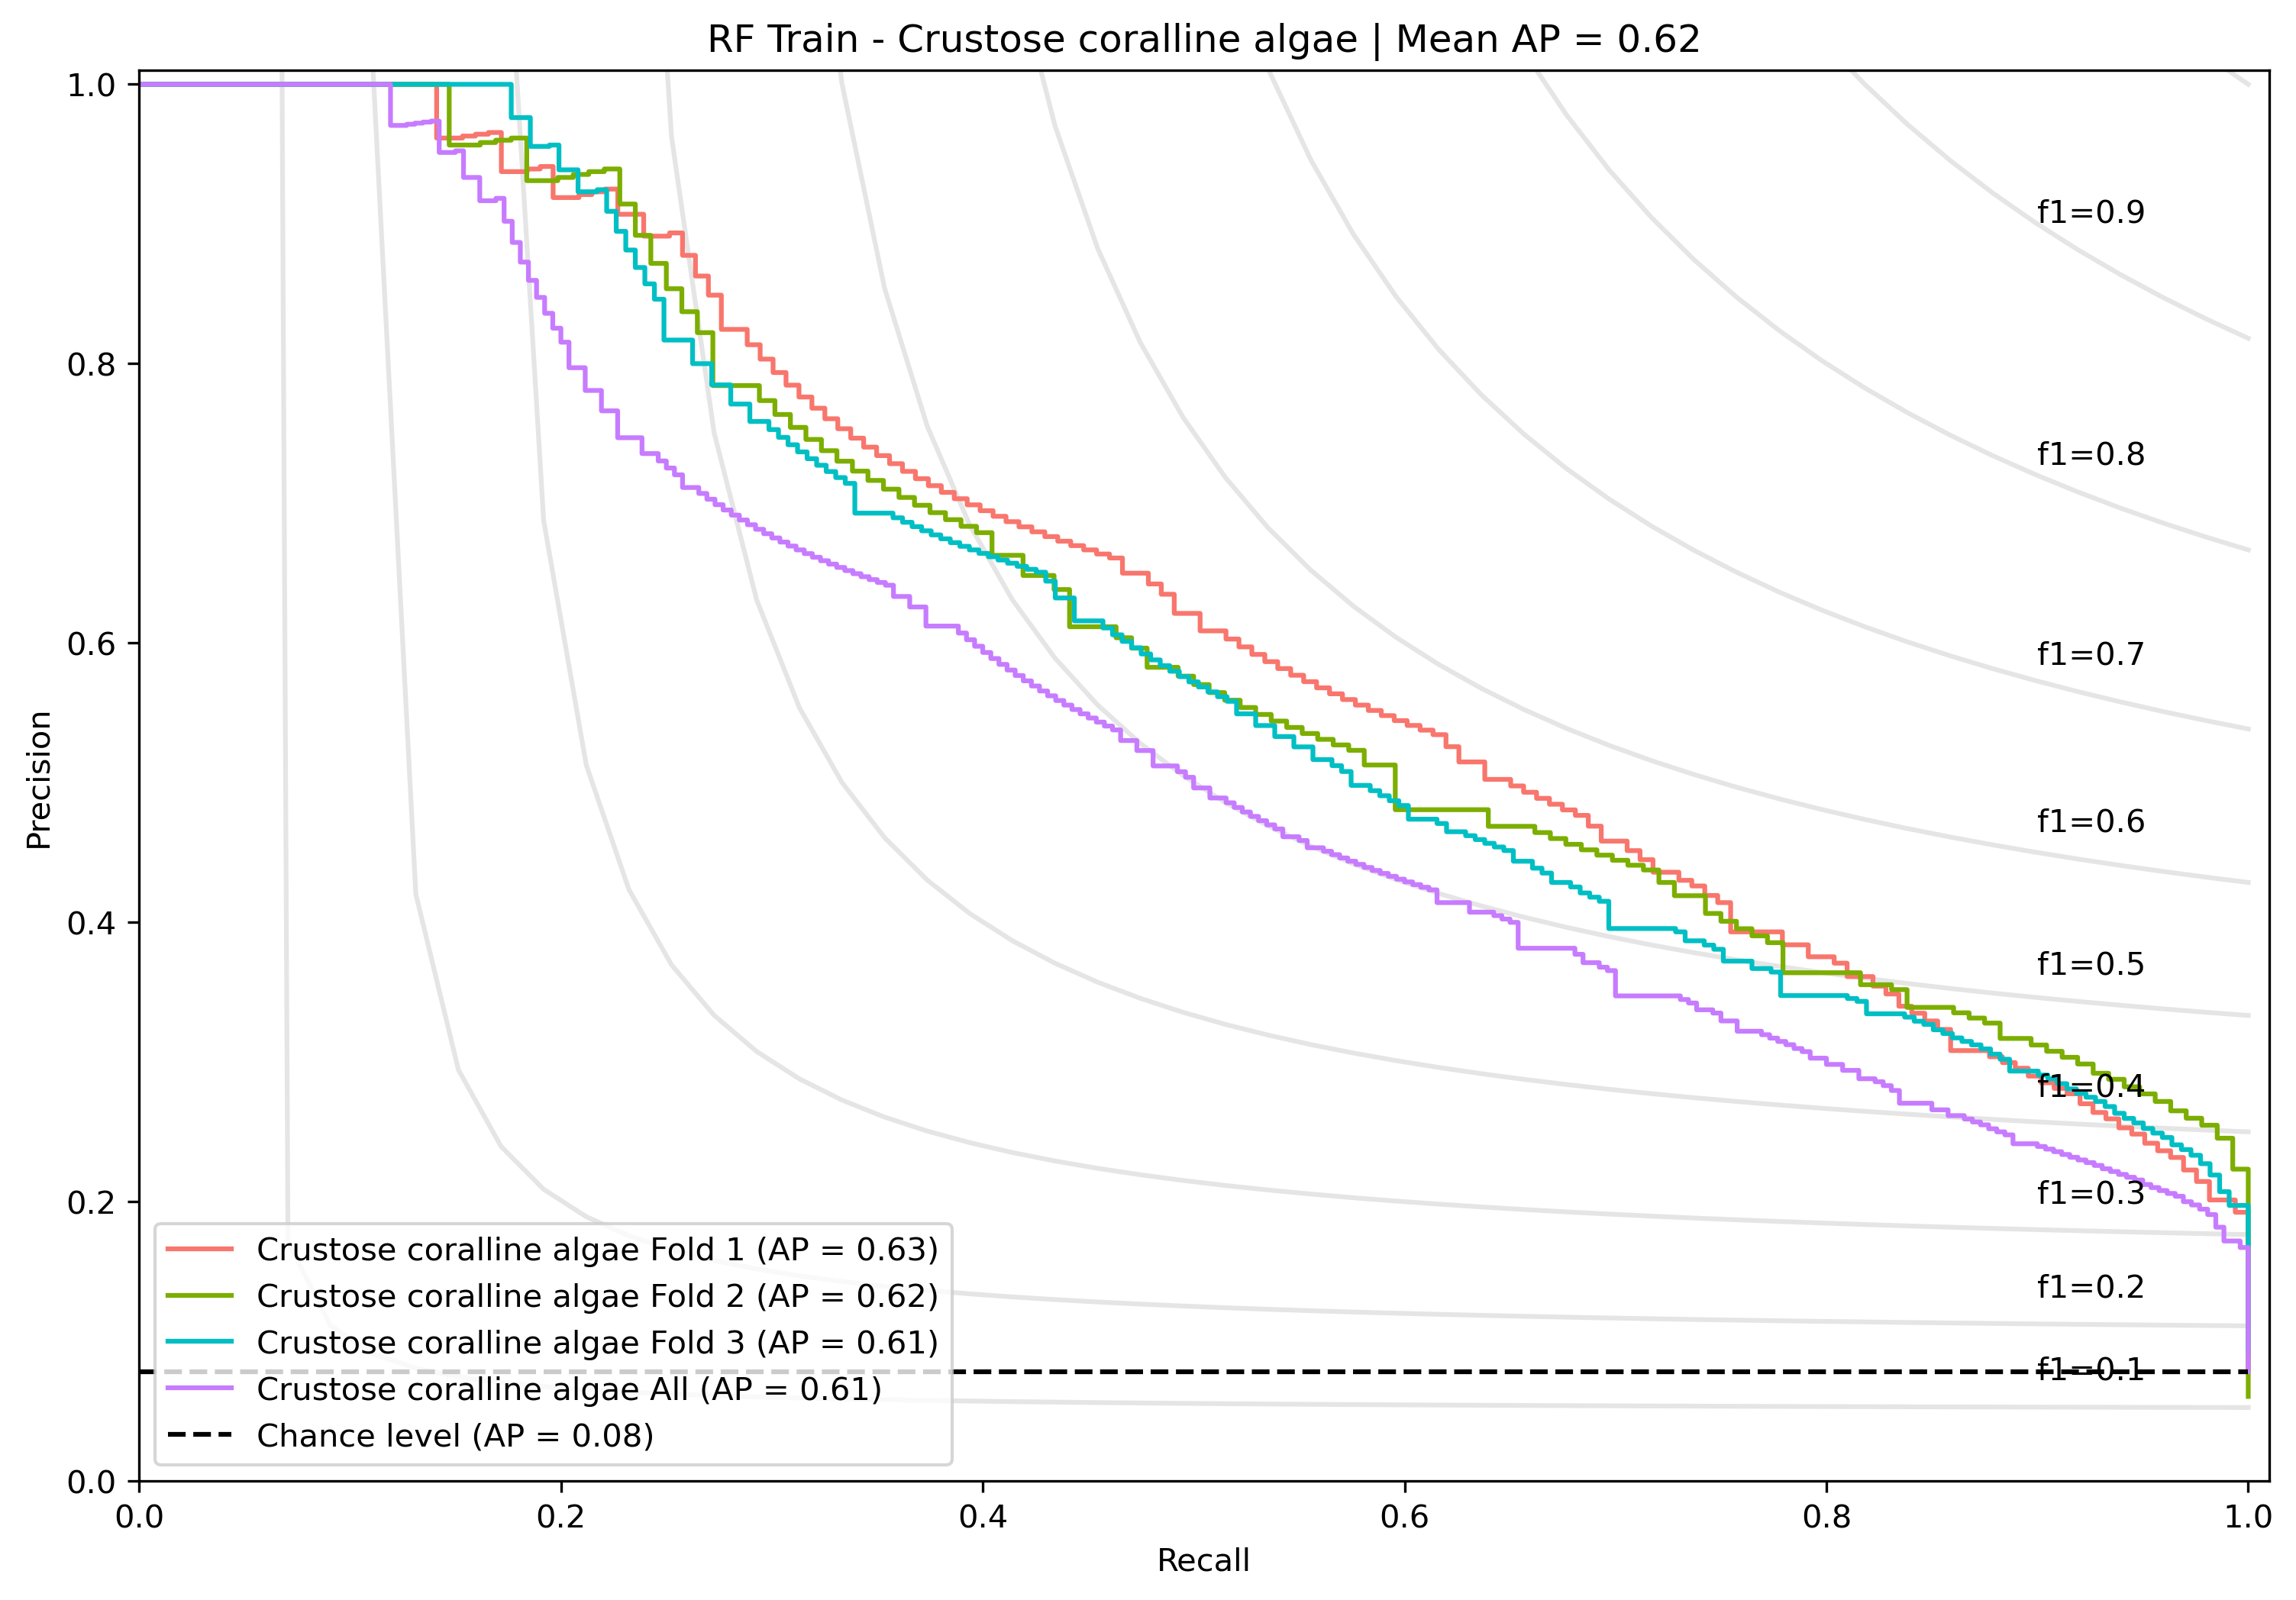
\includegraphics{03-Chapitre3/figures/supplementary/03-precision_recall_curve_train_rf_Crustose coralline algae.png}
\caption{AUPRC curves of the explanatory power for the Crustose
coralline algae. The grey lines represent isolines of
F1-score.}\label{fig:chap3figS26}
}
\end{figure}

\begin{figure}
\hypertarget{fig:chap3figS27}{%
\centering
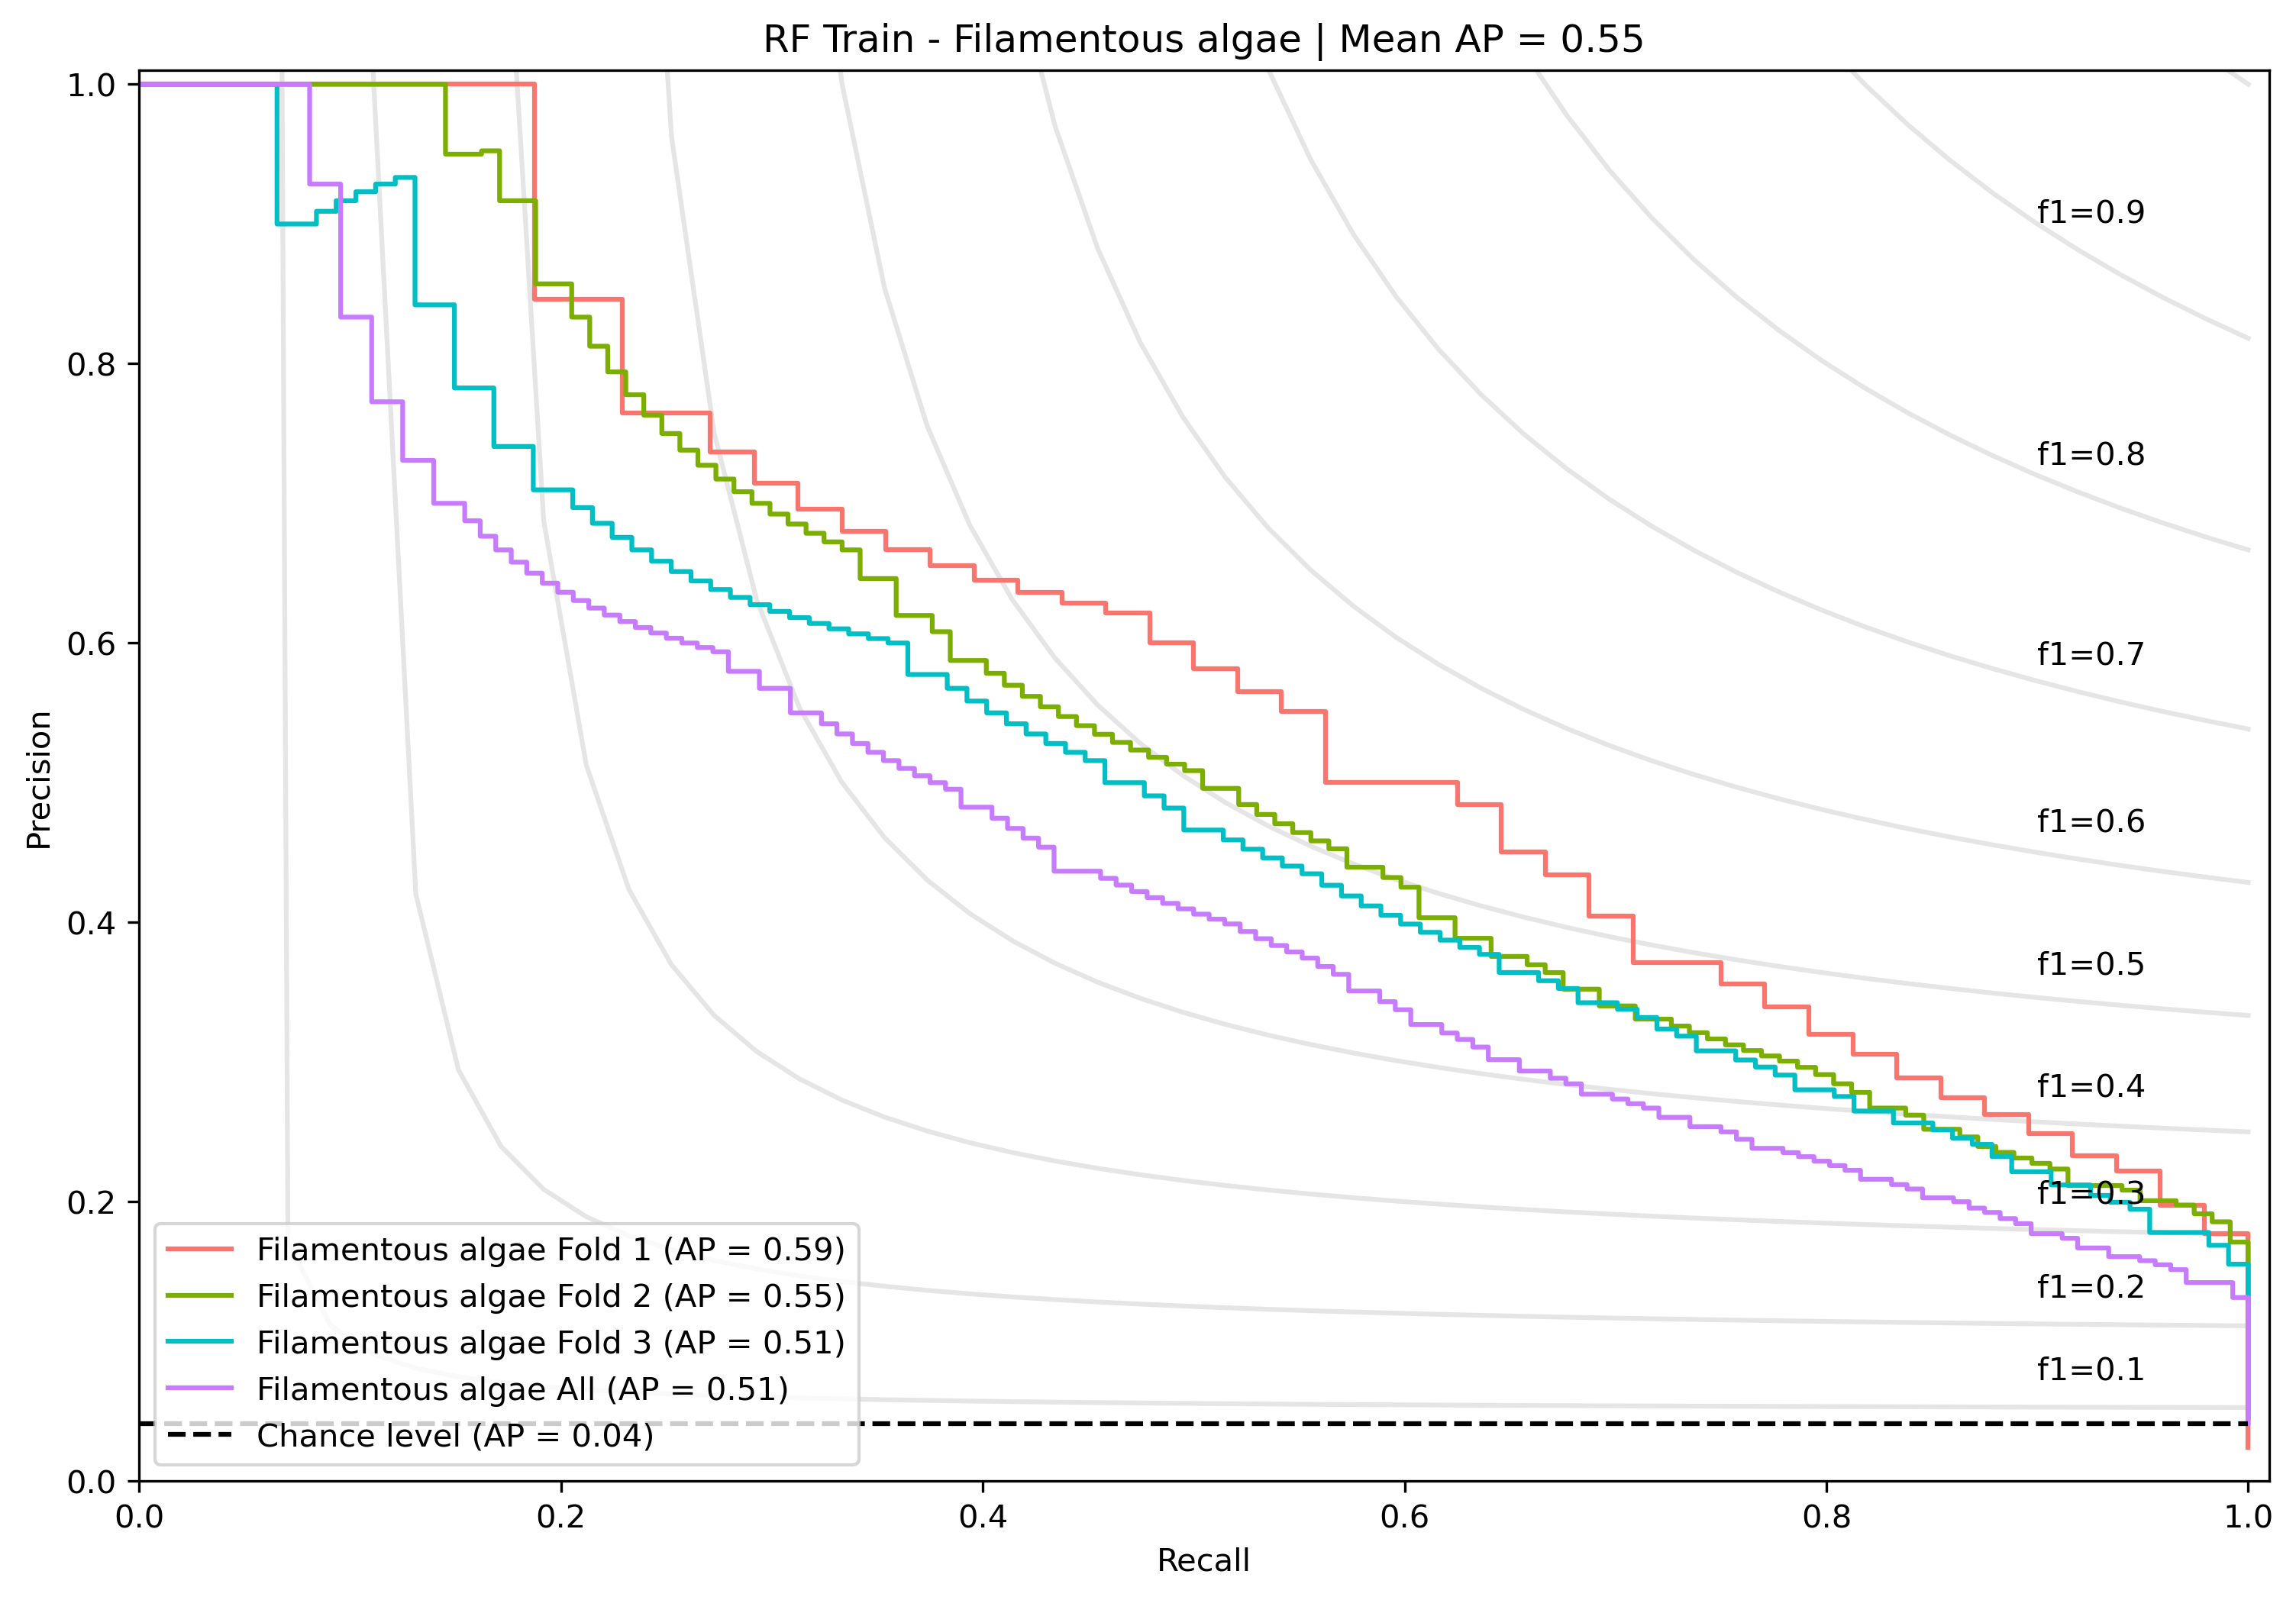
\includegraphics{03-Chapitre3/figures/supplementary/03-precision_recall_curve_train_rf_Filamentous algae.png}
\caption{AUPRC curves of the explanatory power for the Filamentous
algae. The grey lines represent isolines of
F1-score.}\label{fig:chap3figS27}
}
\end{figure}

\begin{figure}
\hypertarget{fig:chap3figS28}{%
\centering
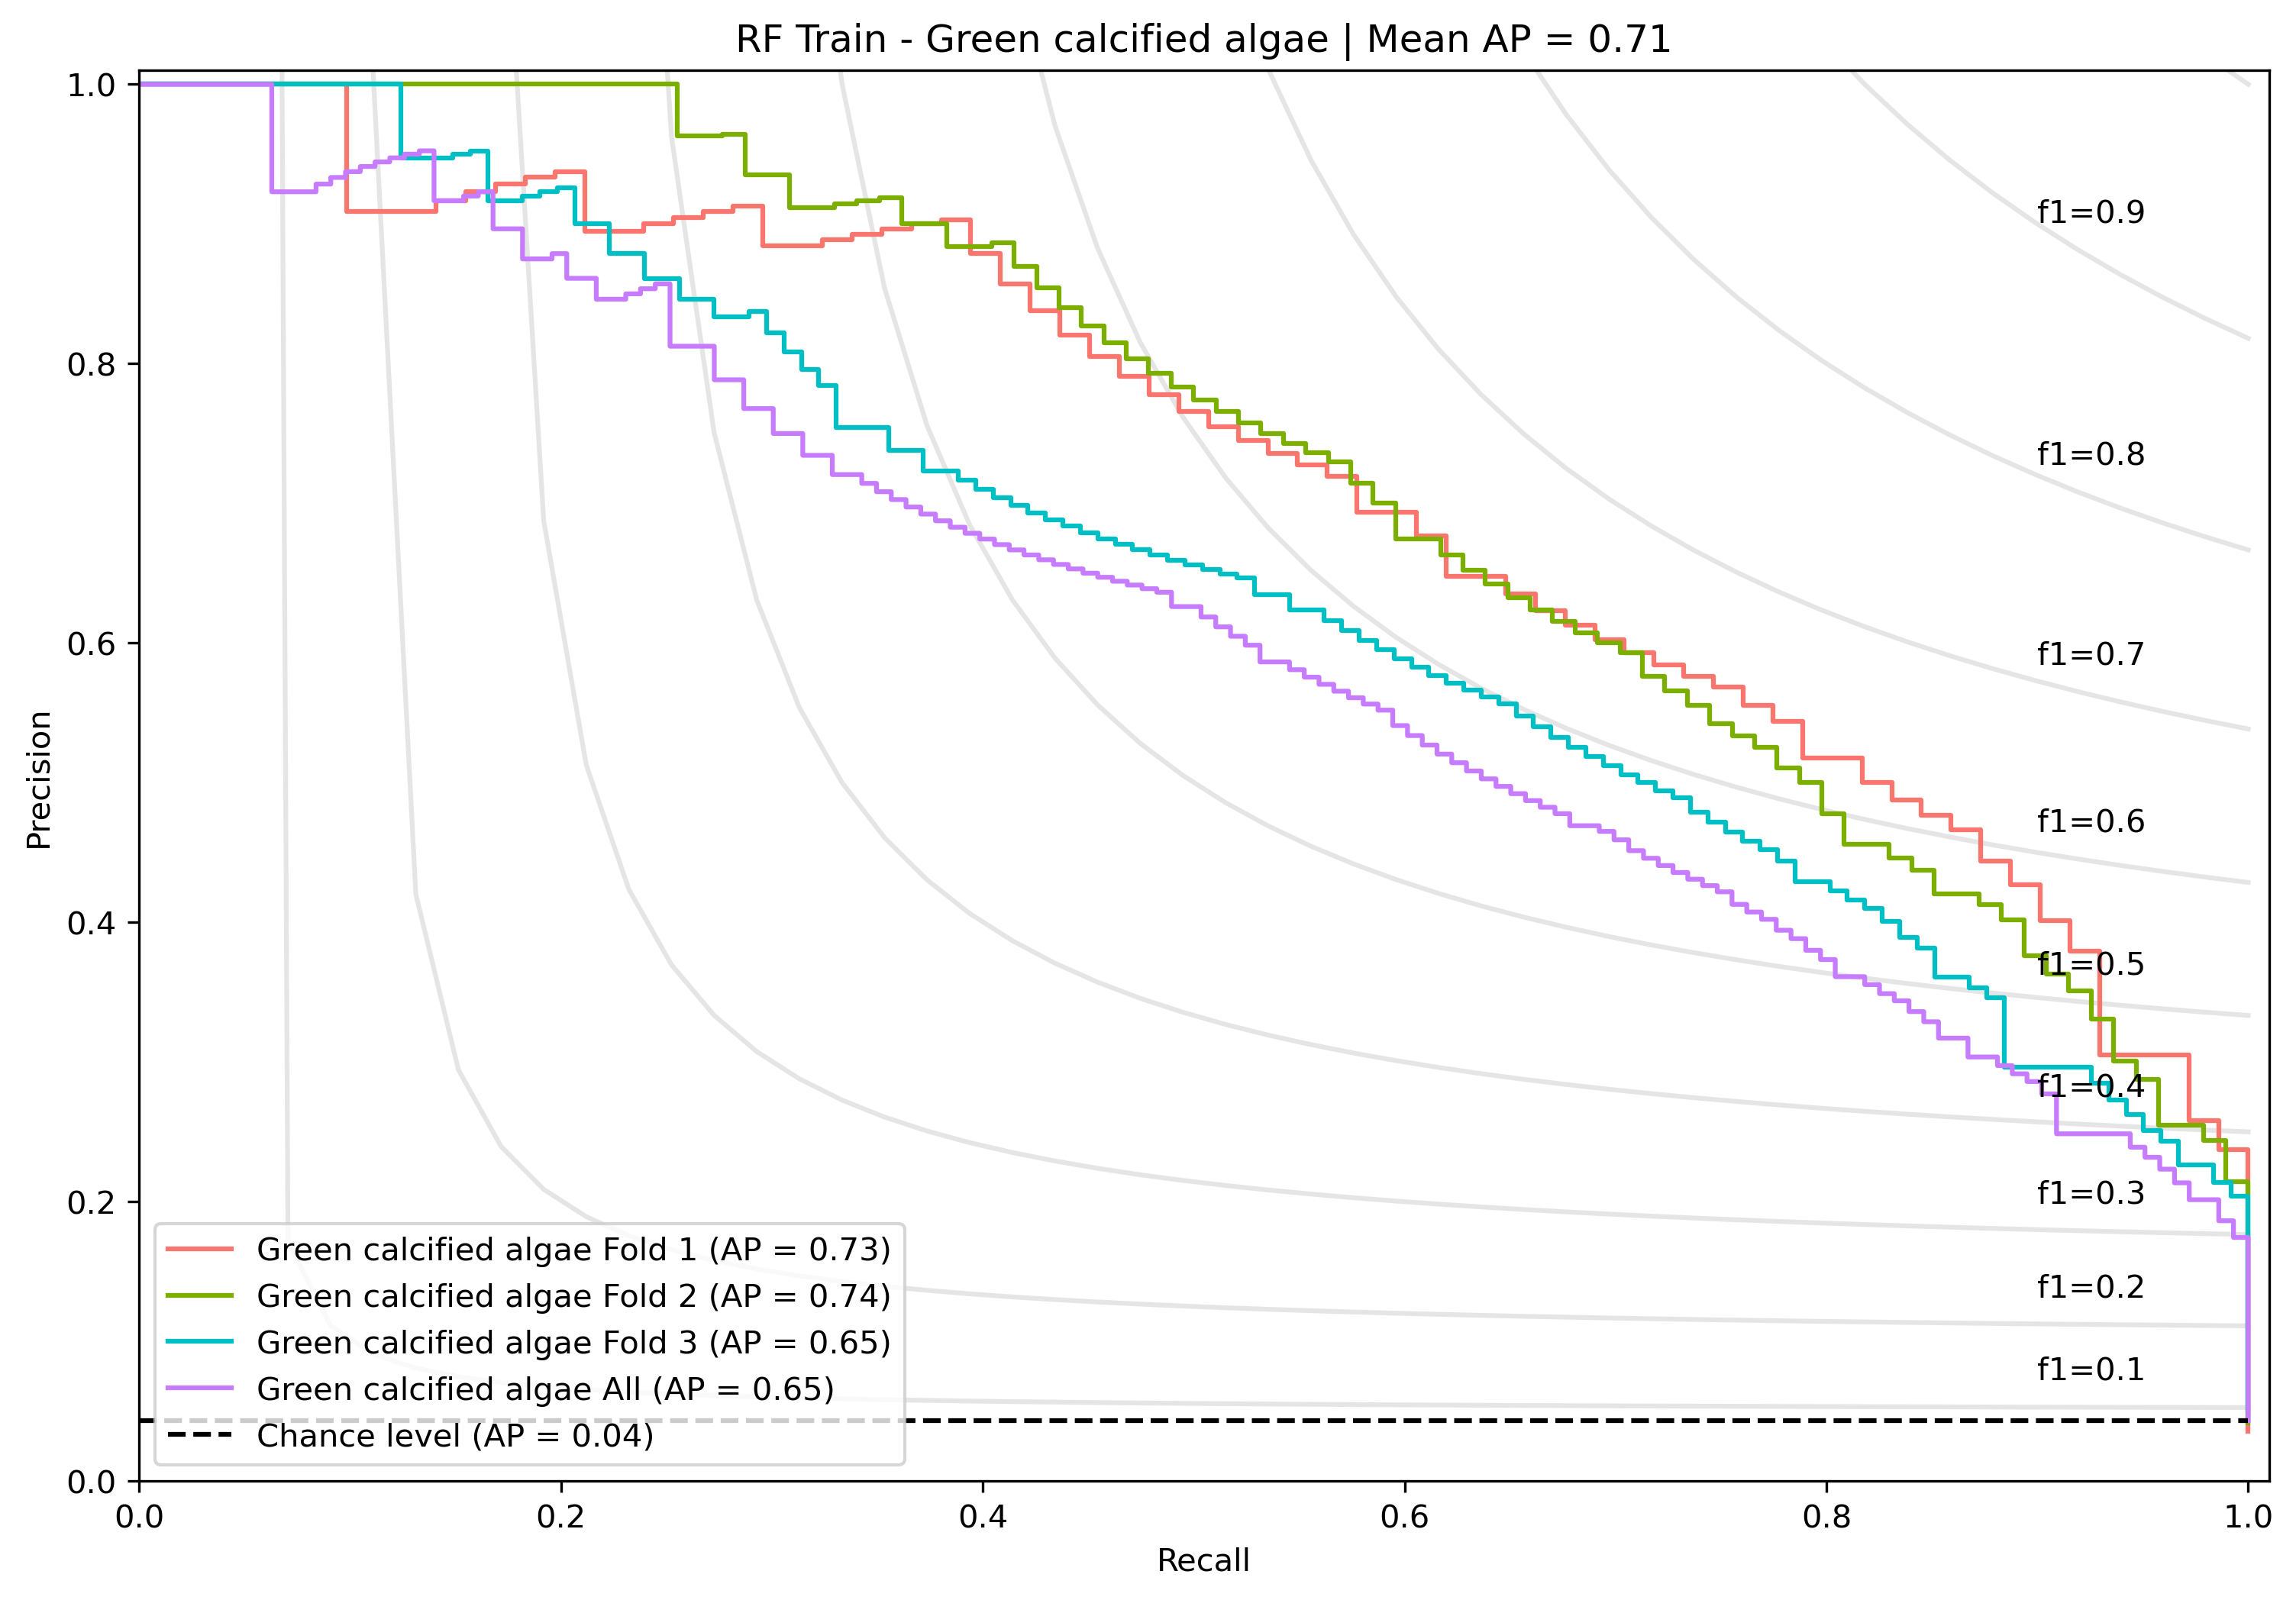
\includegraphics{03-Chapitre3/figures/supplementary/03-precision_recall_curve_train_rf_Green calcified algae.png}
\caption{AUPRC curves of the explanatory power for the Green Calcified
algae. The grey lines represent isolines of
F1-score.}\label{fig:chap3figS28}
}
\end{figure}

\begin{figure}
\hypertarget{fig:chap3figS29}{%
\centering
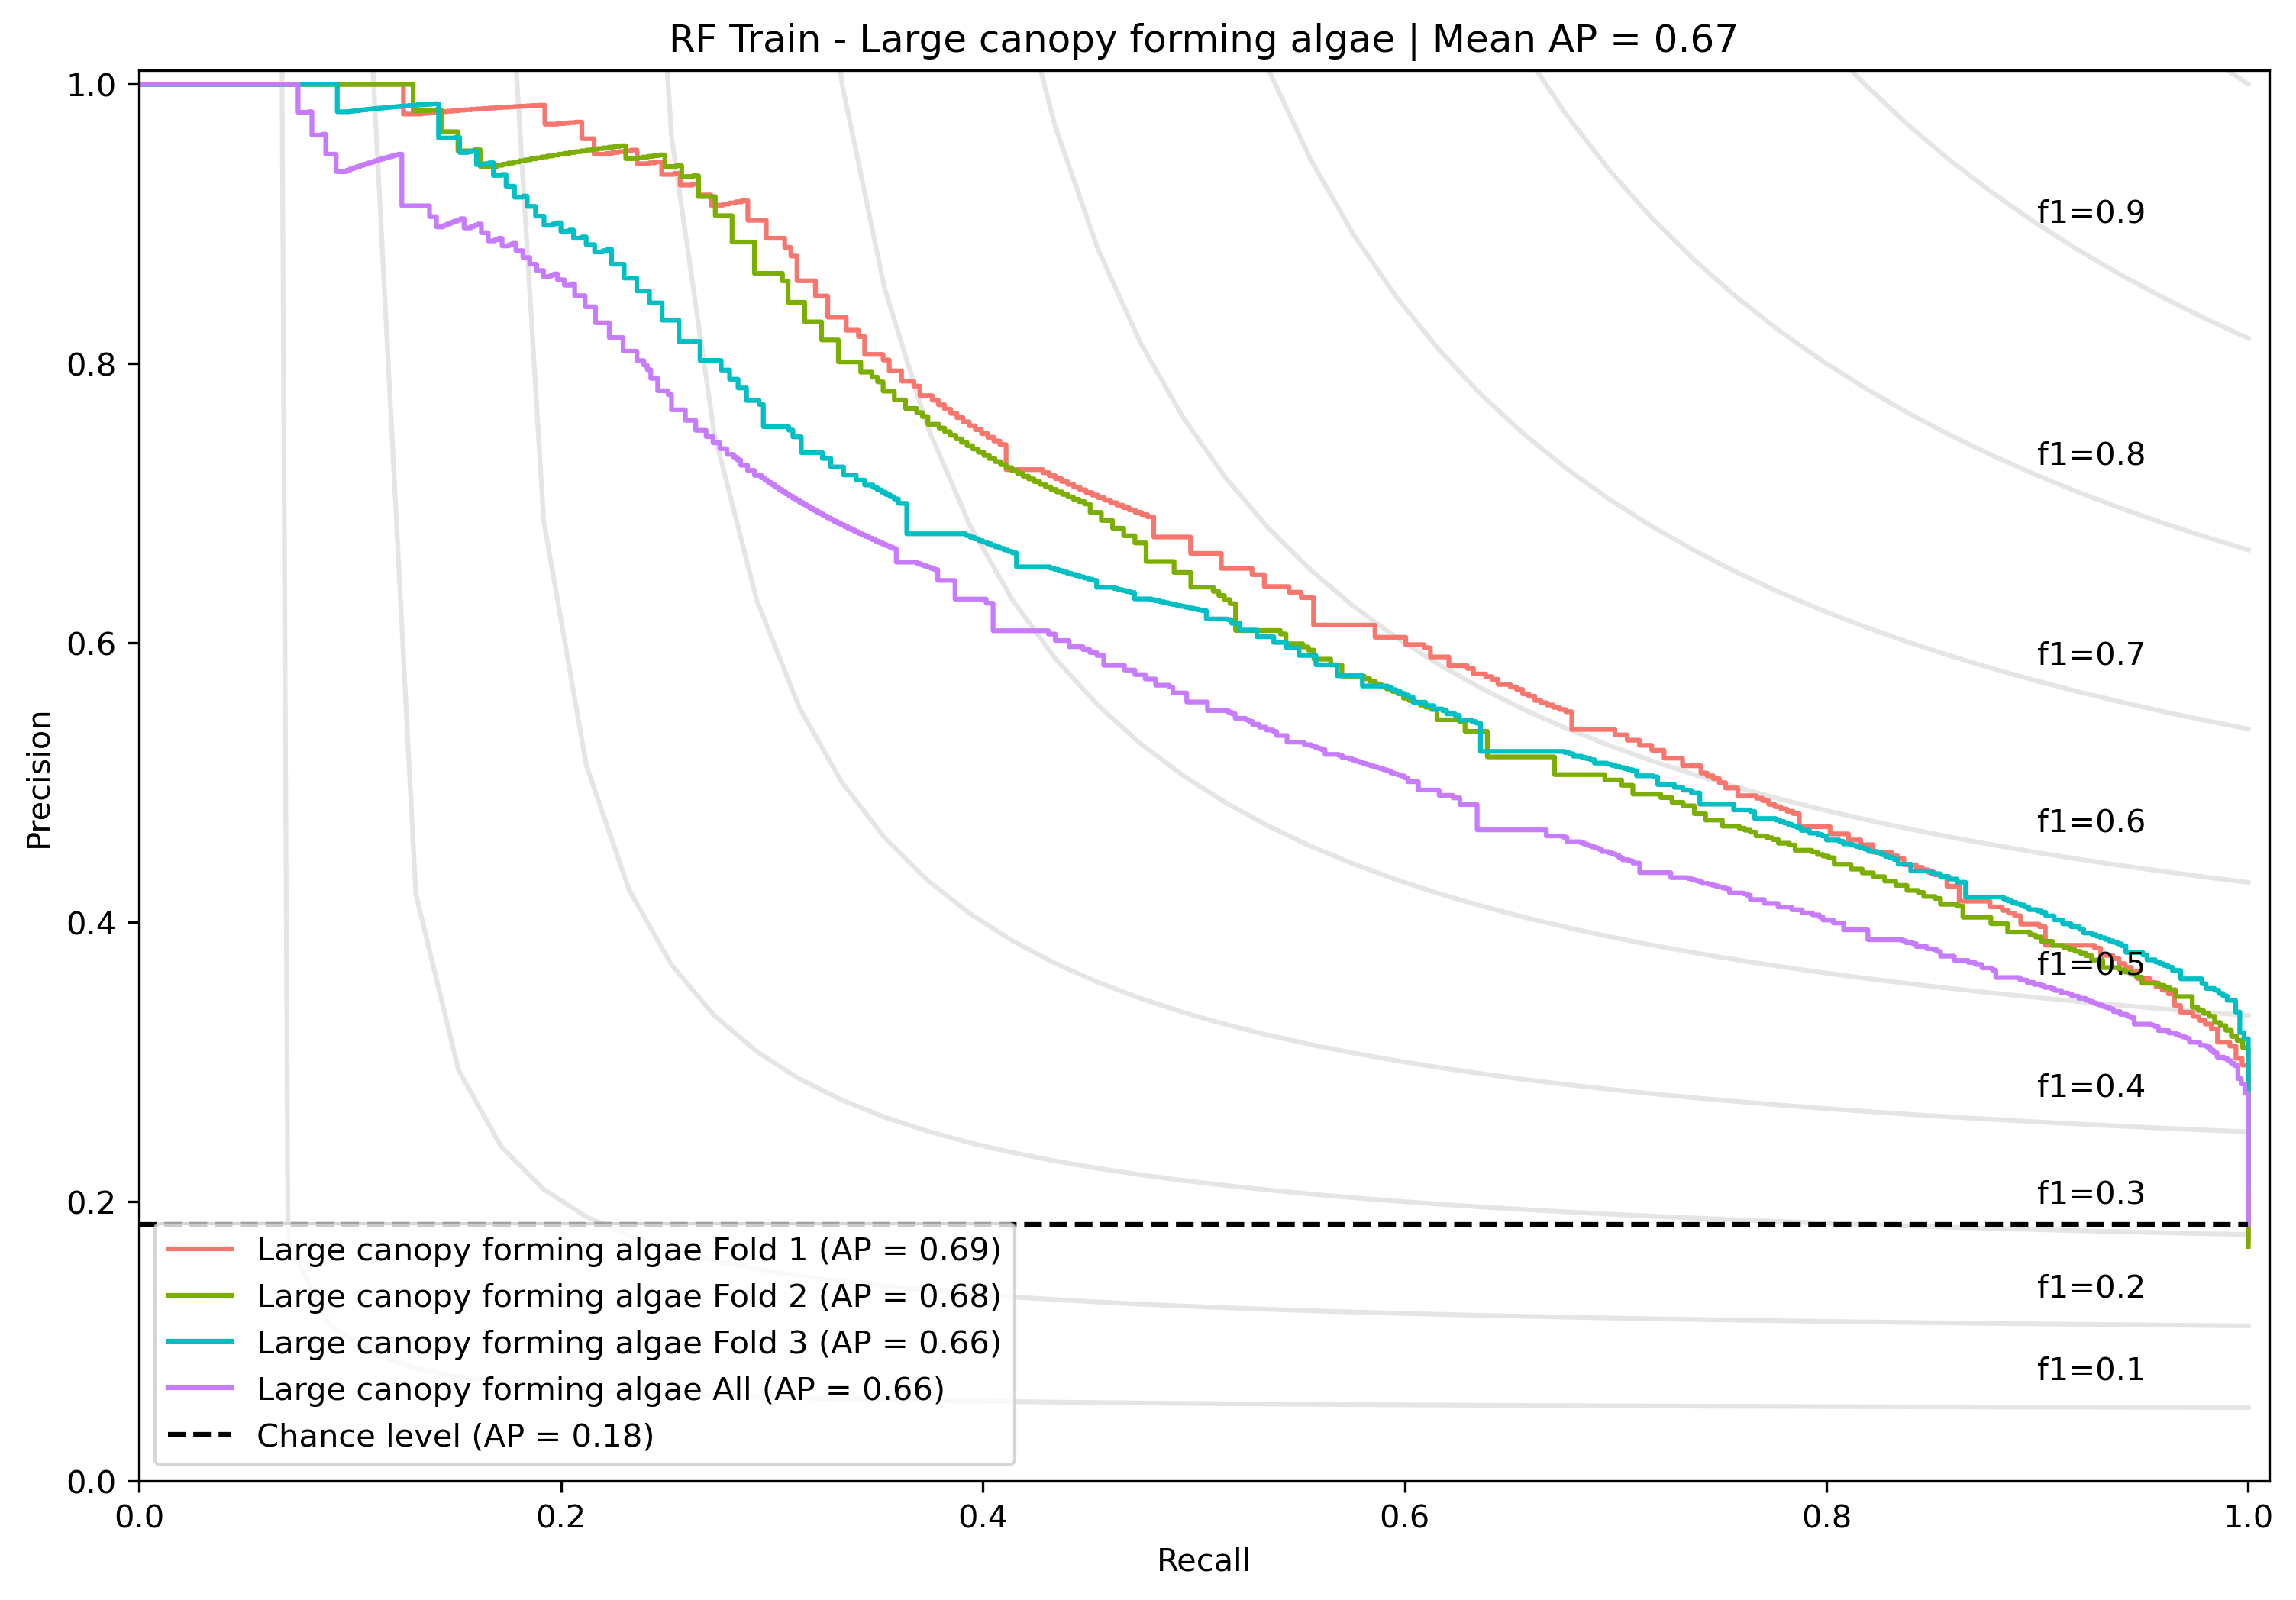
\includegraphics{03-Chapitre3/figures/supplementary/03-precision_recall_curve_train_rf_Large canopy forming algae.png}
\caption{AUPRC curves of the explanatory power for the Large canopy
forming algae. The grey lines represent isolines of
F1-score.}\label{fig:chap3figS29}
}
\end{figure}

\begin{figure}
\hypertarget{fig:chap3figS30}{%
\centering
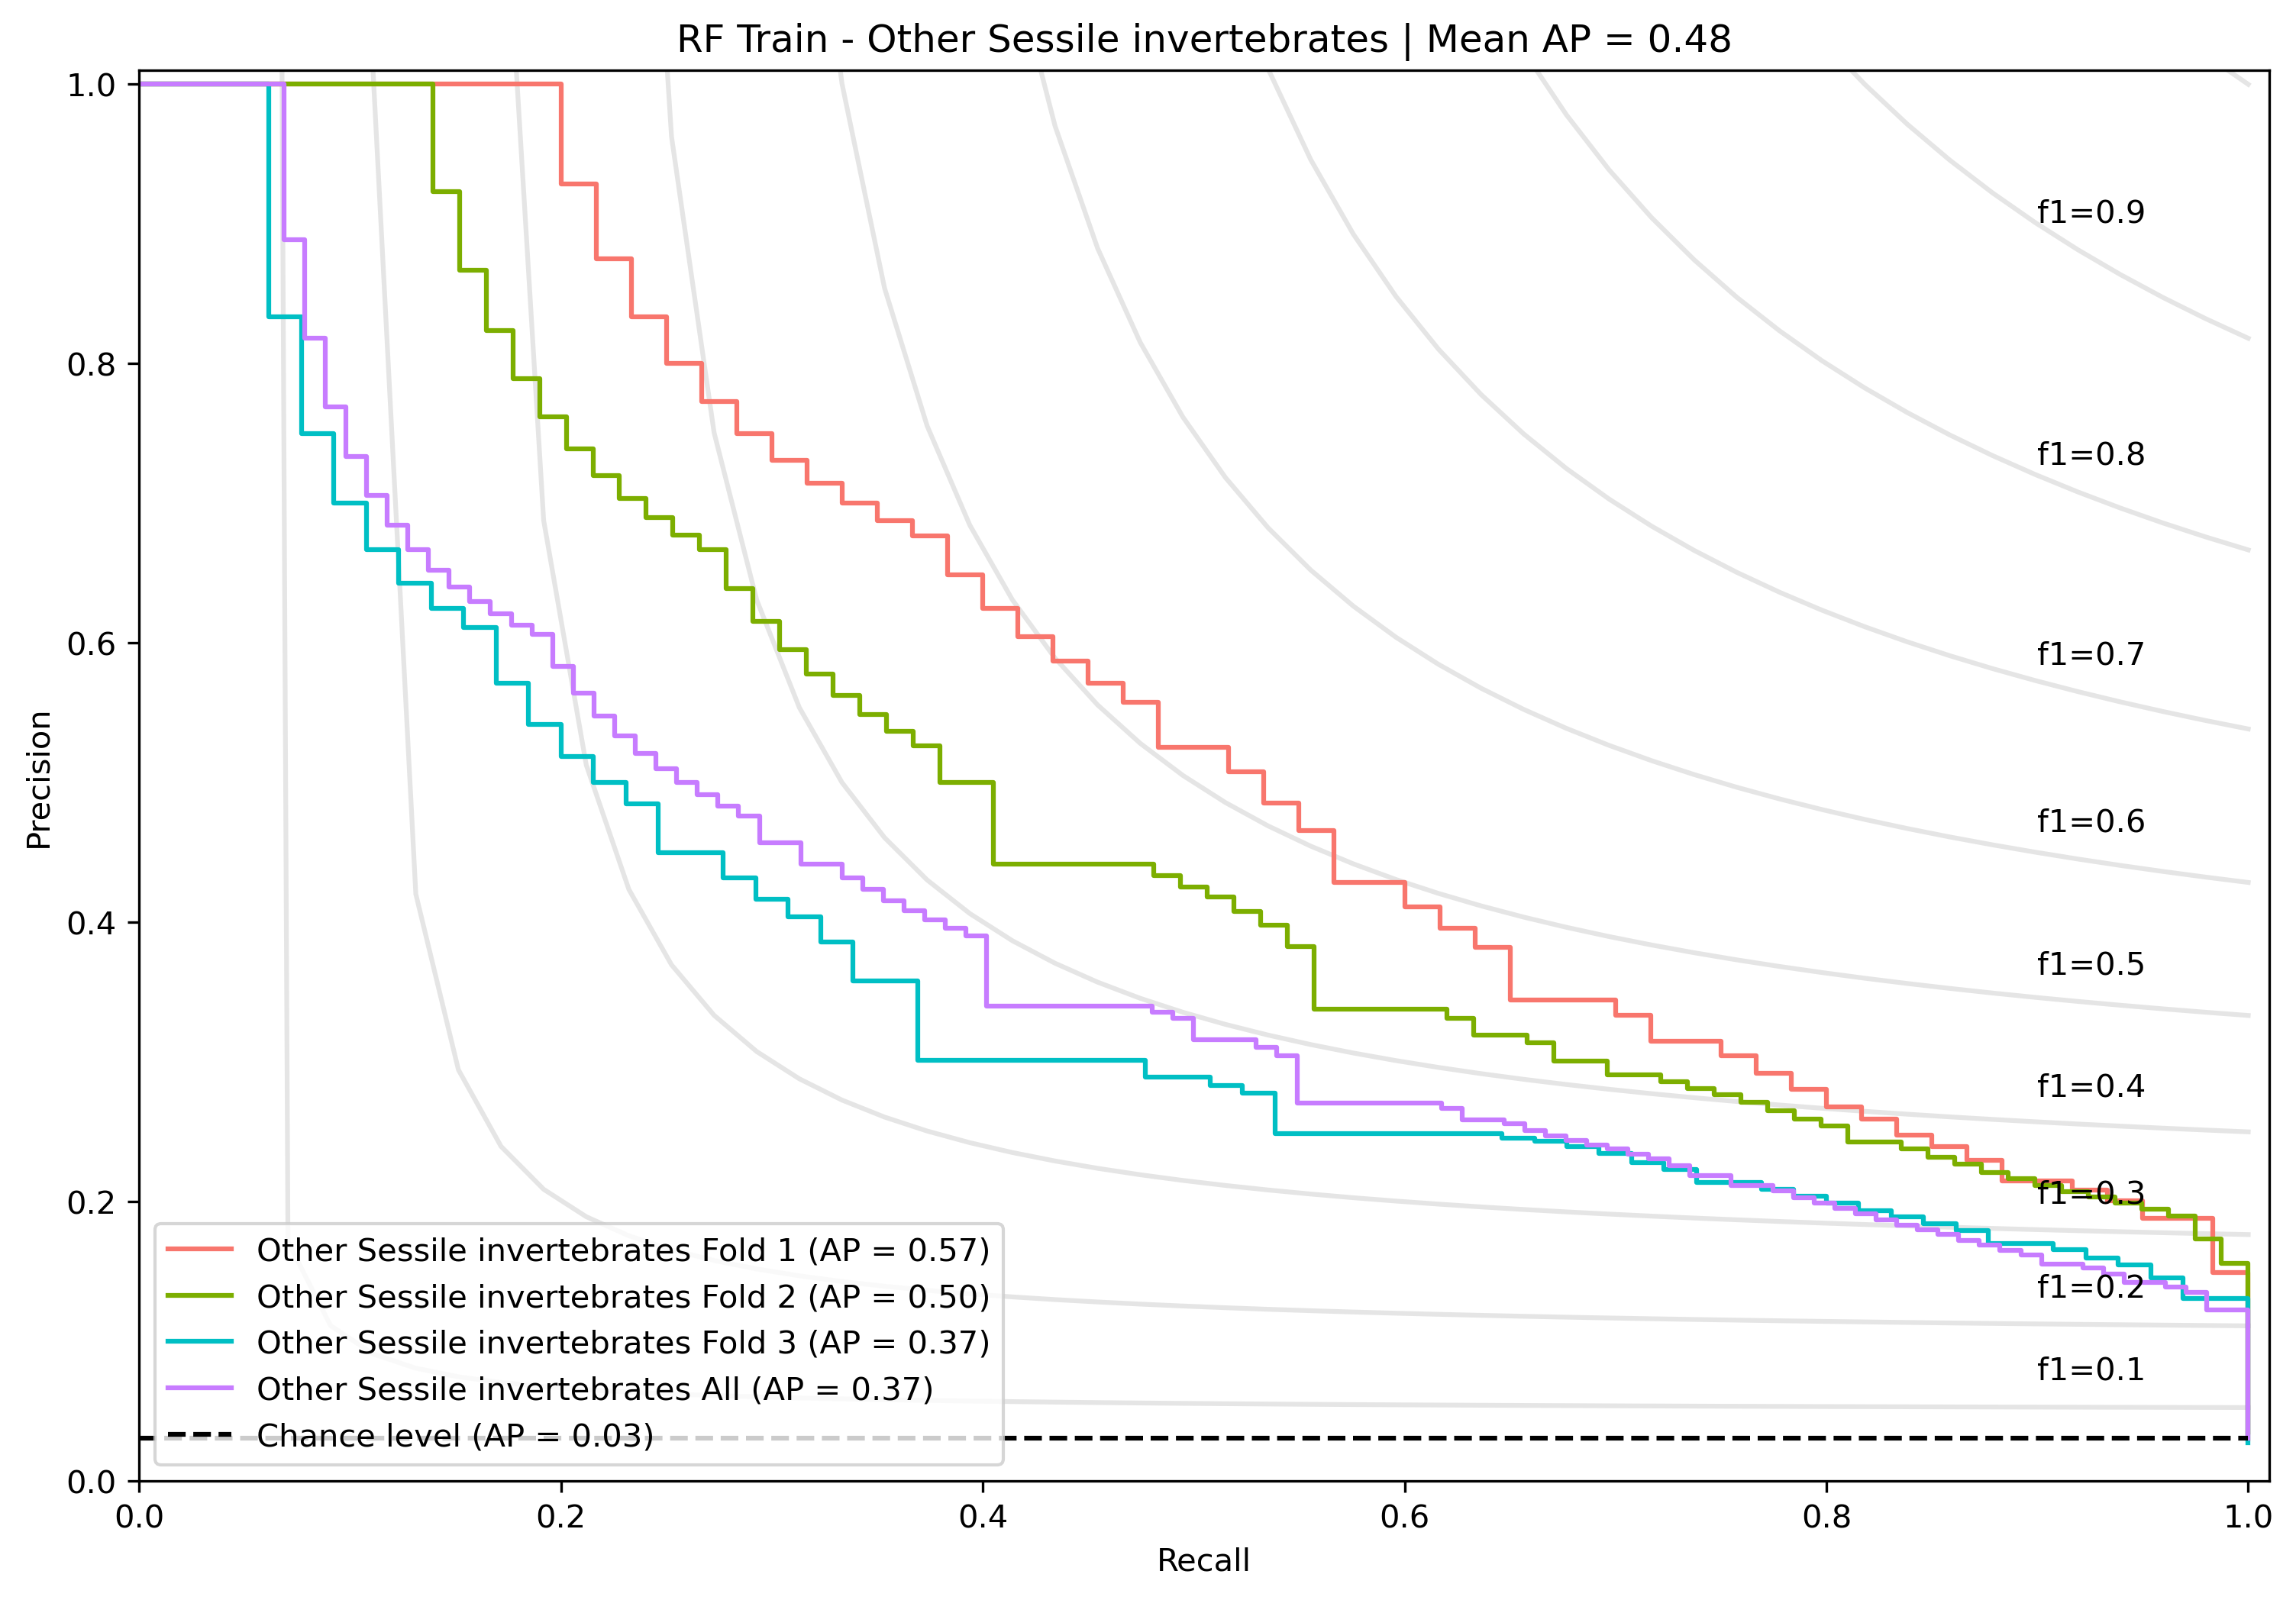
\includegraphics{03-Chapitre3/figures/supplementary/03-precision_recall_curve_train_rf_Other Sessile invertebrates.png}
\caption{AUPRC curves of the explanatory power for the Other Sessile
invertebrates. The grey lines represent isolines of
F1-score.}\label{fig:chap3figS30}
}
\end{figure}

\begin{figure}
\hypertarget{fig:chap3figS31}{%
\centering
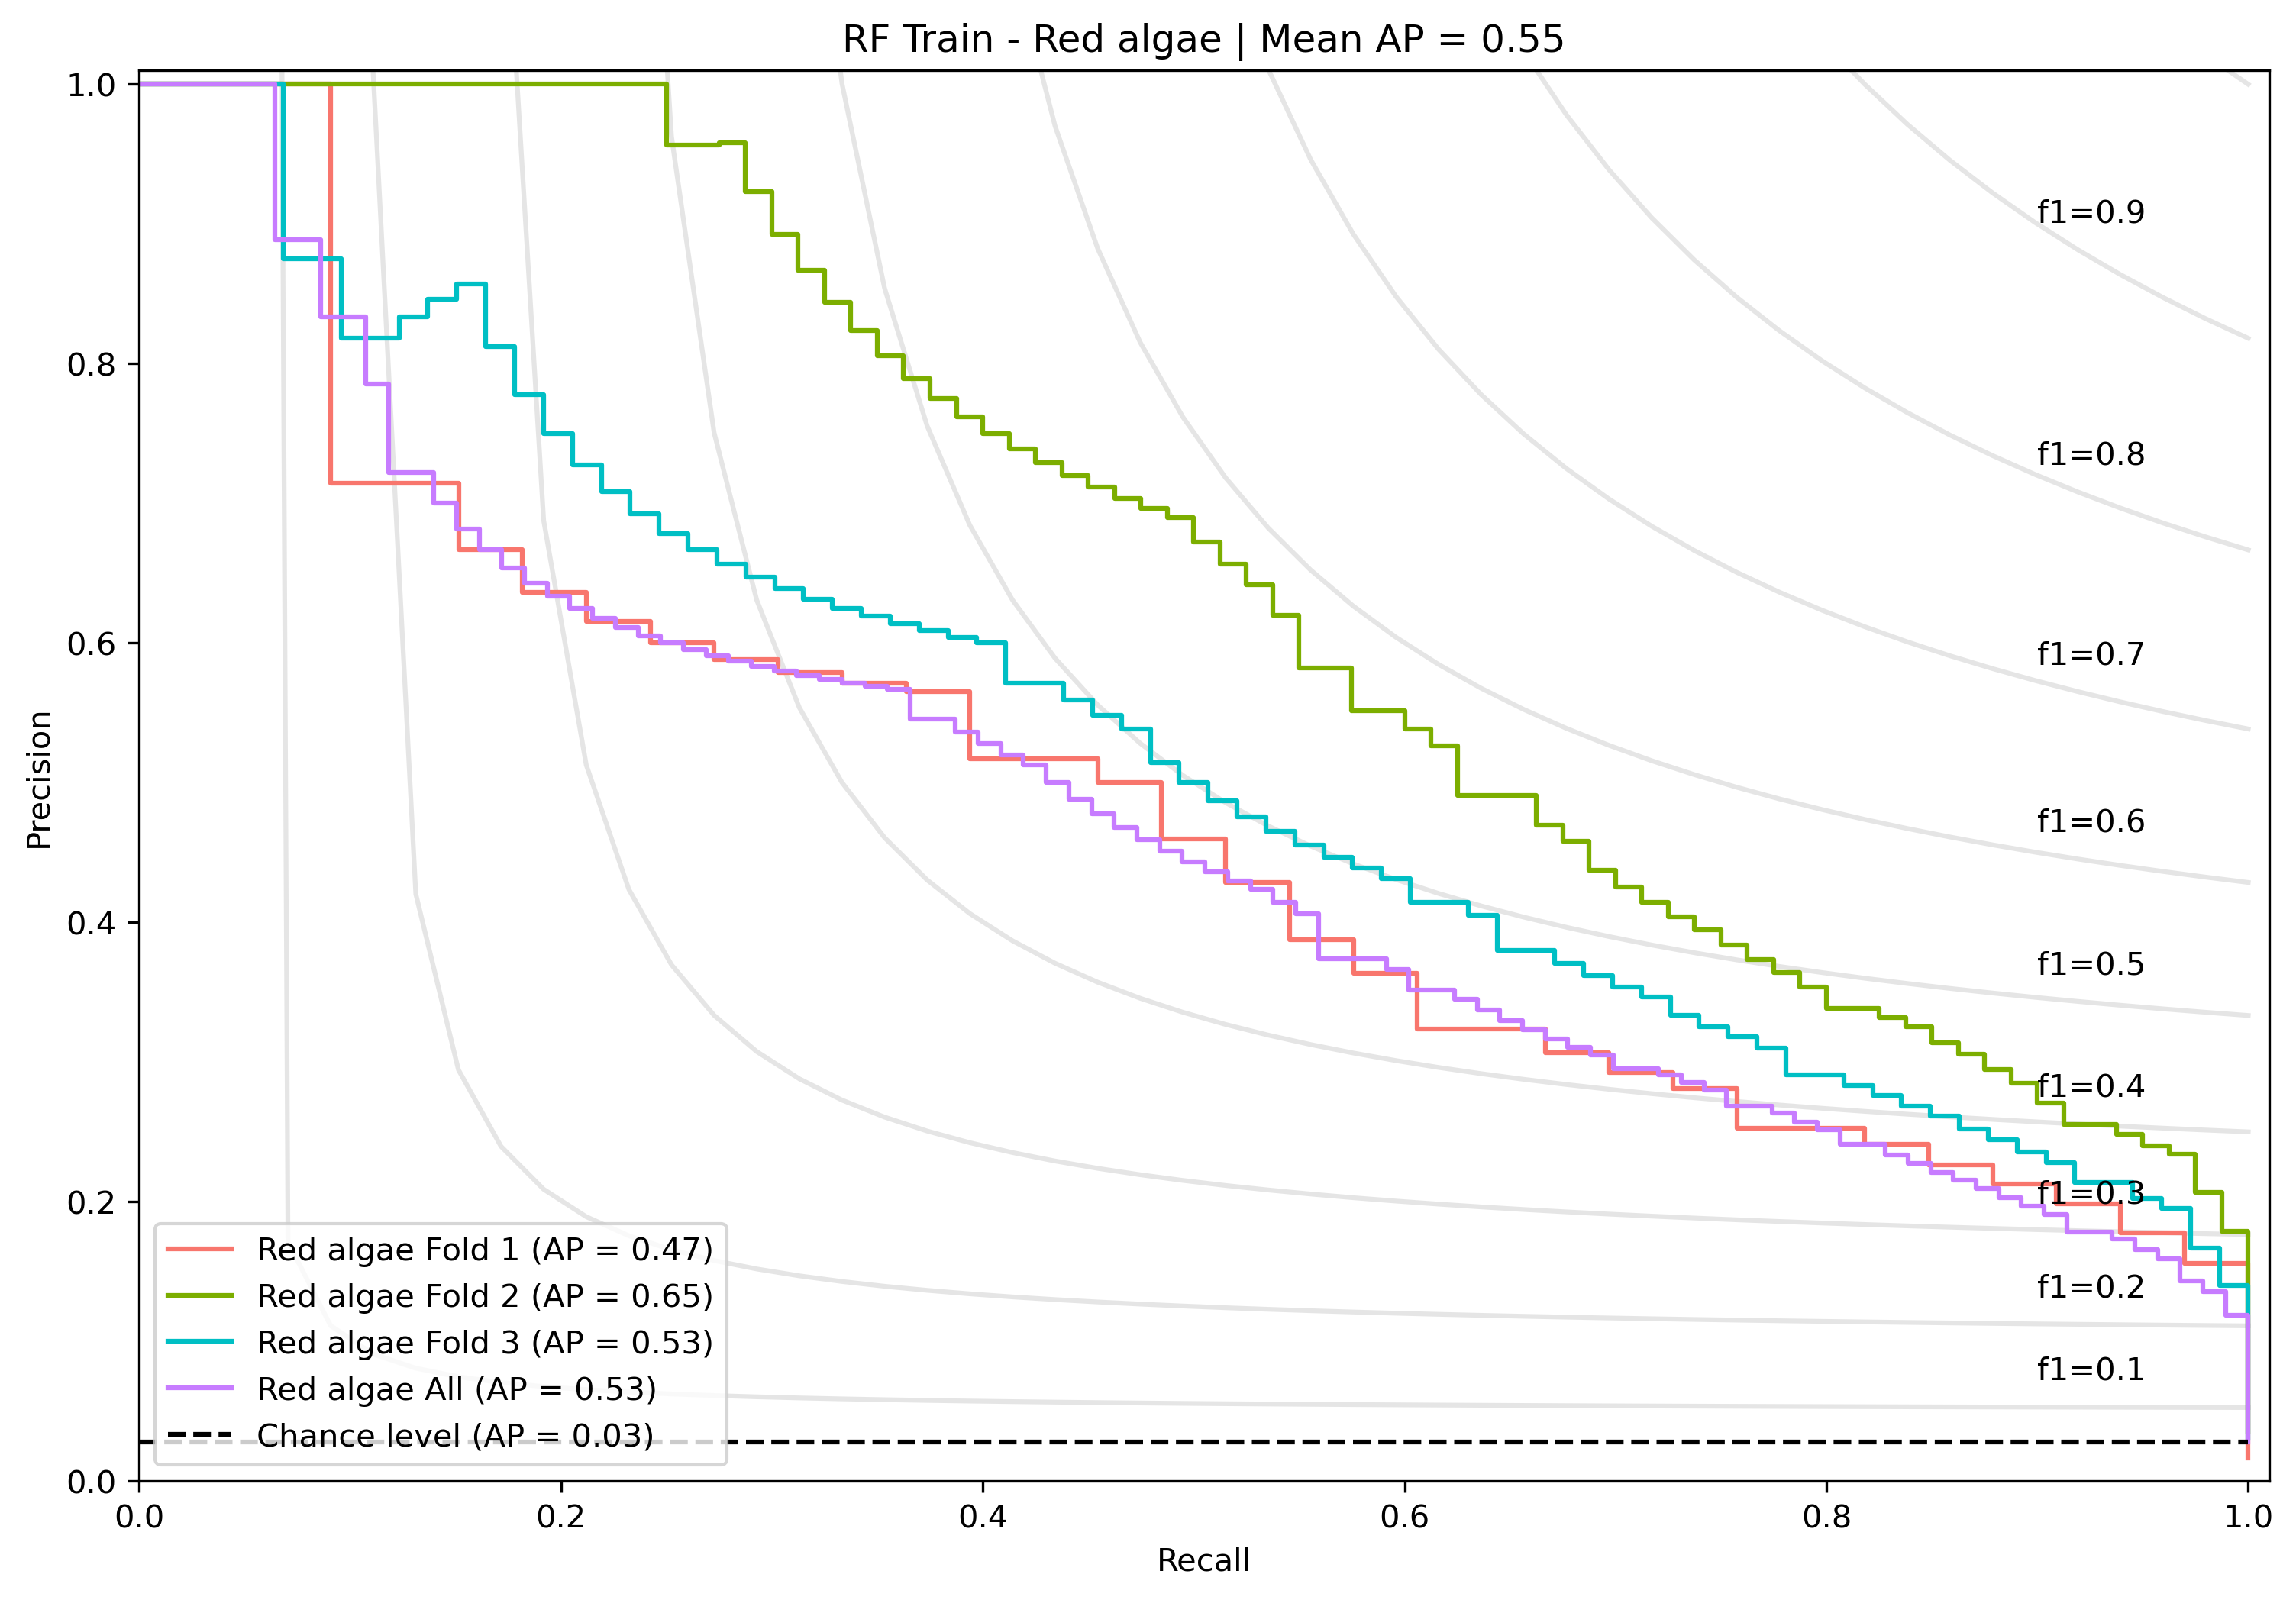
\includegraphics{03-Chapitre3/figures/supplementary/03-precision_recall_curve_train_rf_Red algae.png}
\caption{AUPRC curves of the explanatory power for the Red algae. The
grey lines represent isolines of F1-score.}\label{fig:chap3figS31}
}
\end{figure}

\begin{figure}
\hypertarget{fig:chap3figS32}{%
\centering
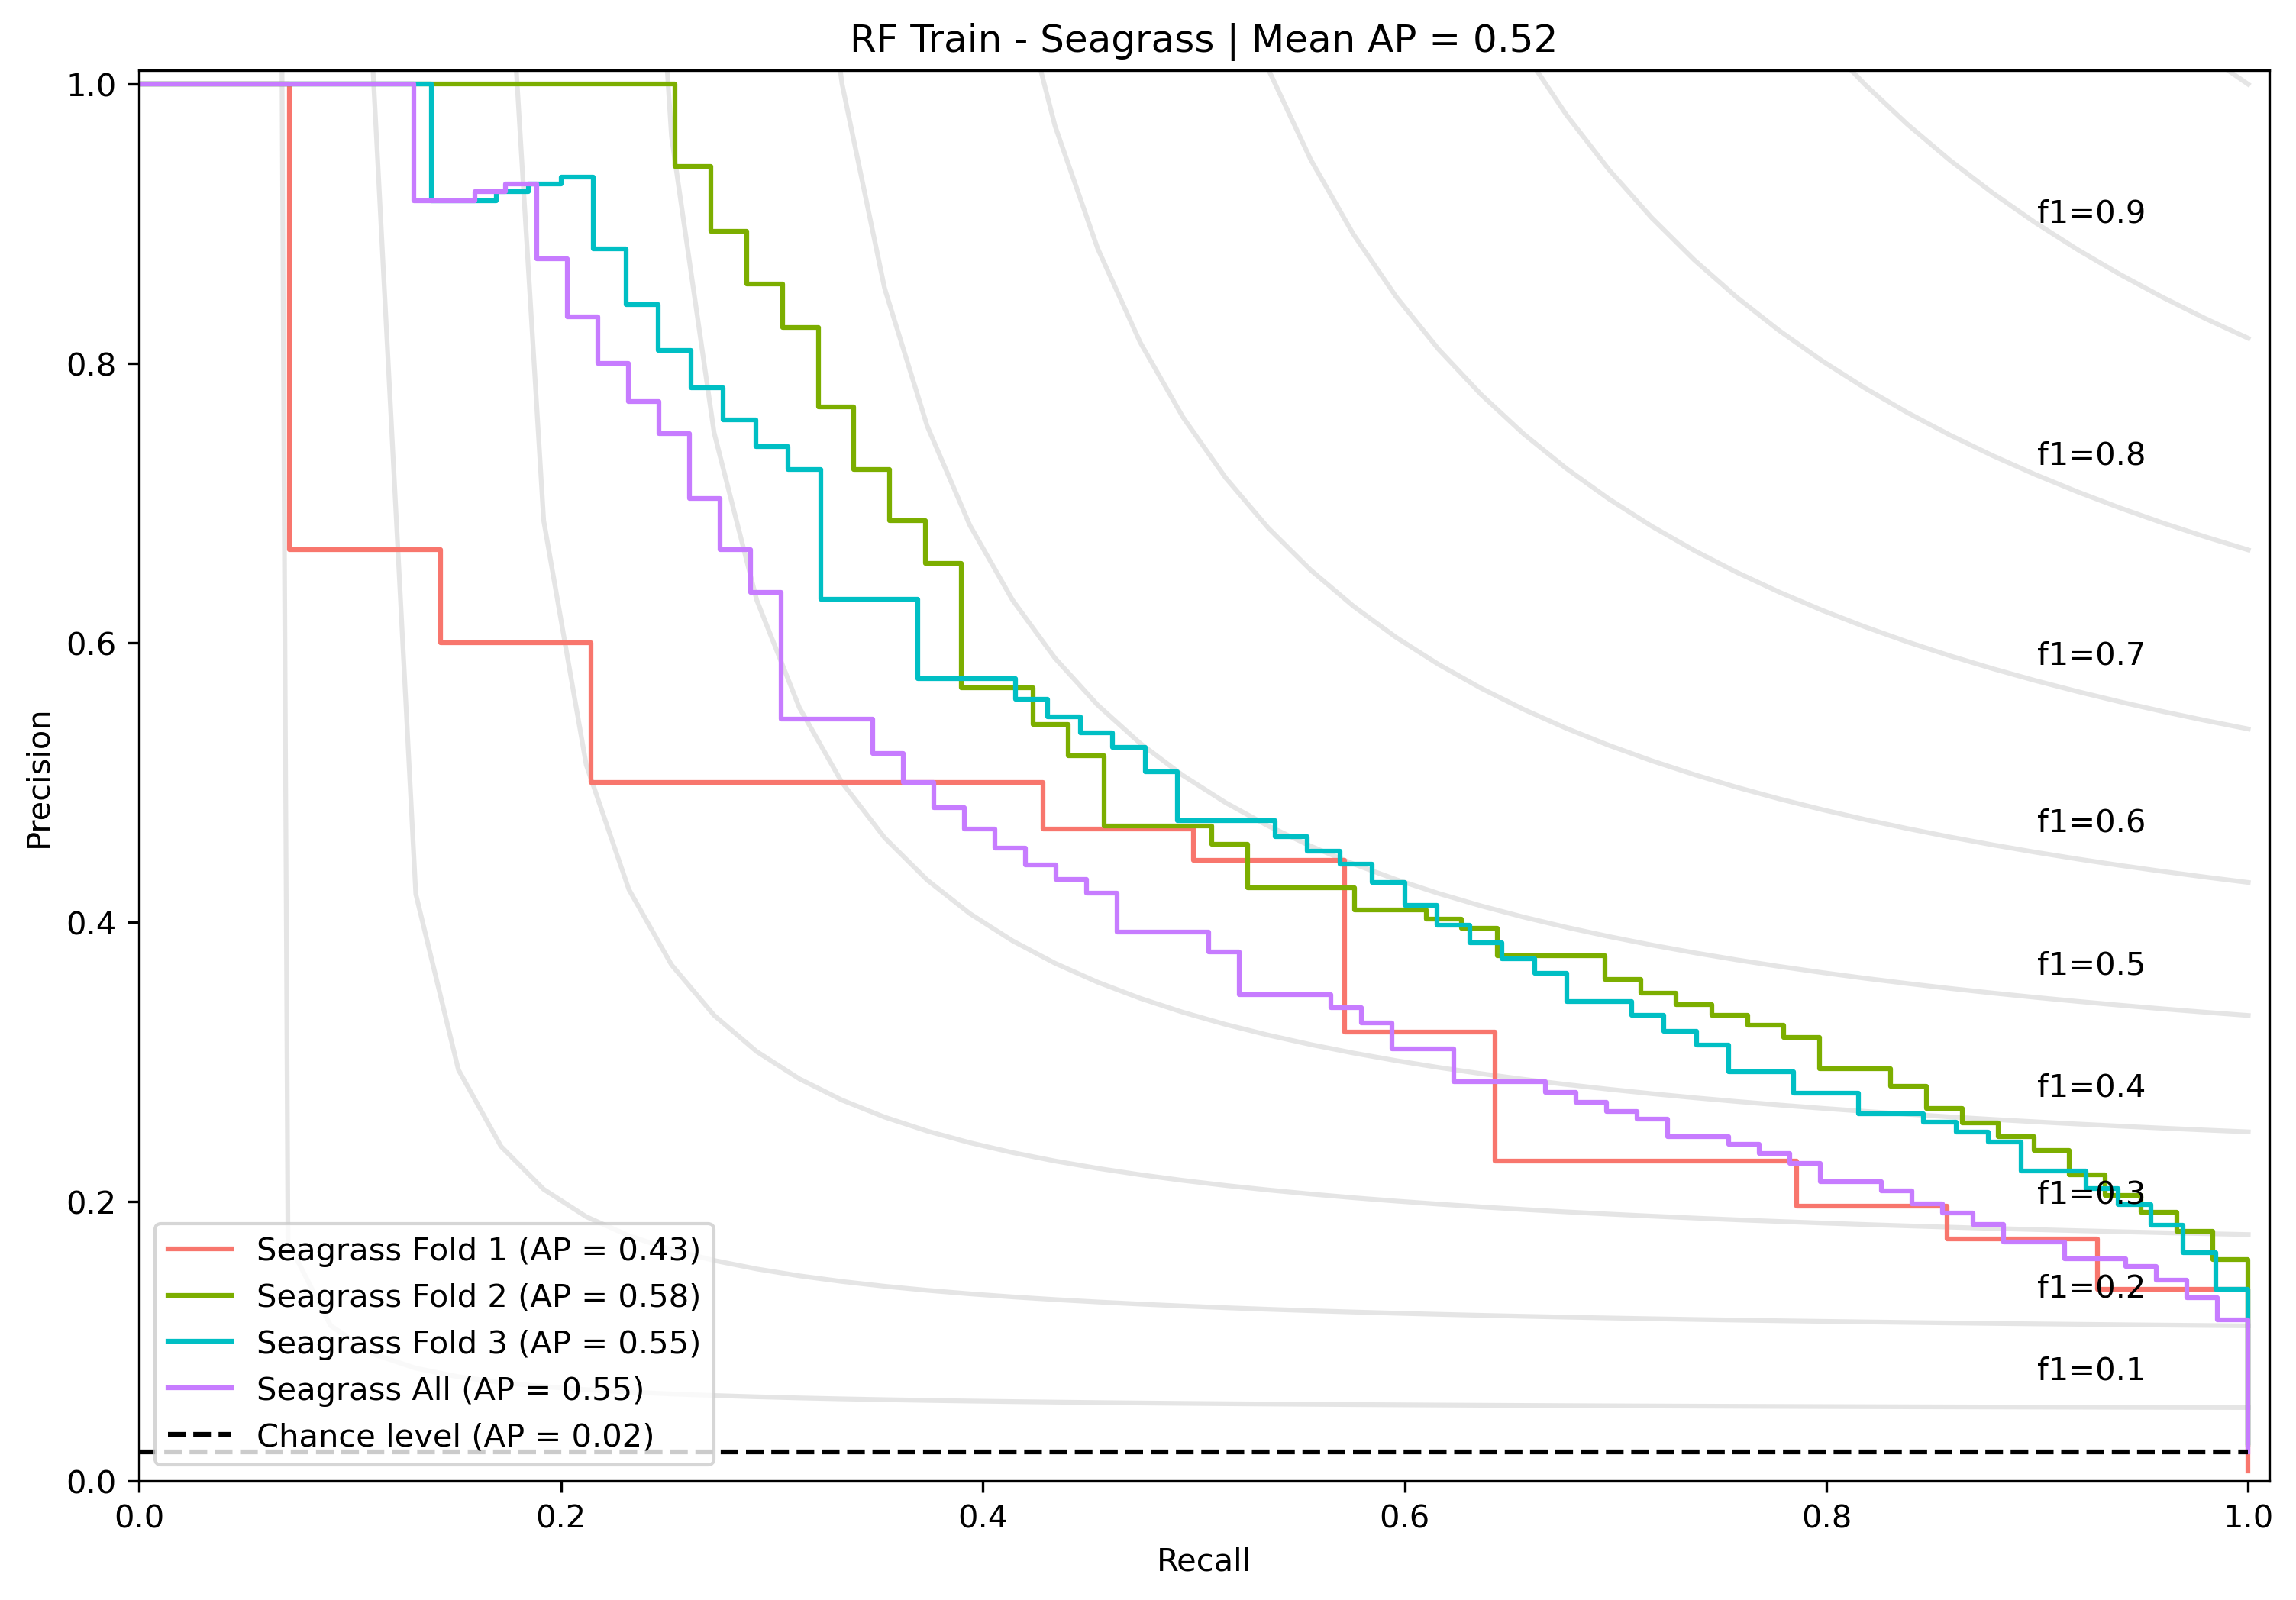
\includegraphics{03-Chapitre3/figures/supplementary/03-precision_recall_curve_train_rf_Seagrass.png}
\caption{AUPRC curves of the explanatory power for the Seagrass. The
grey lines represent isolines of F1-score.}\label{fig:chap3figS32}
}
\end{figure}

\begin{figure}
\hypertarget{fig:chap3figS33}{%
\centering
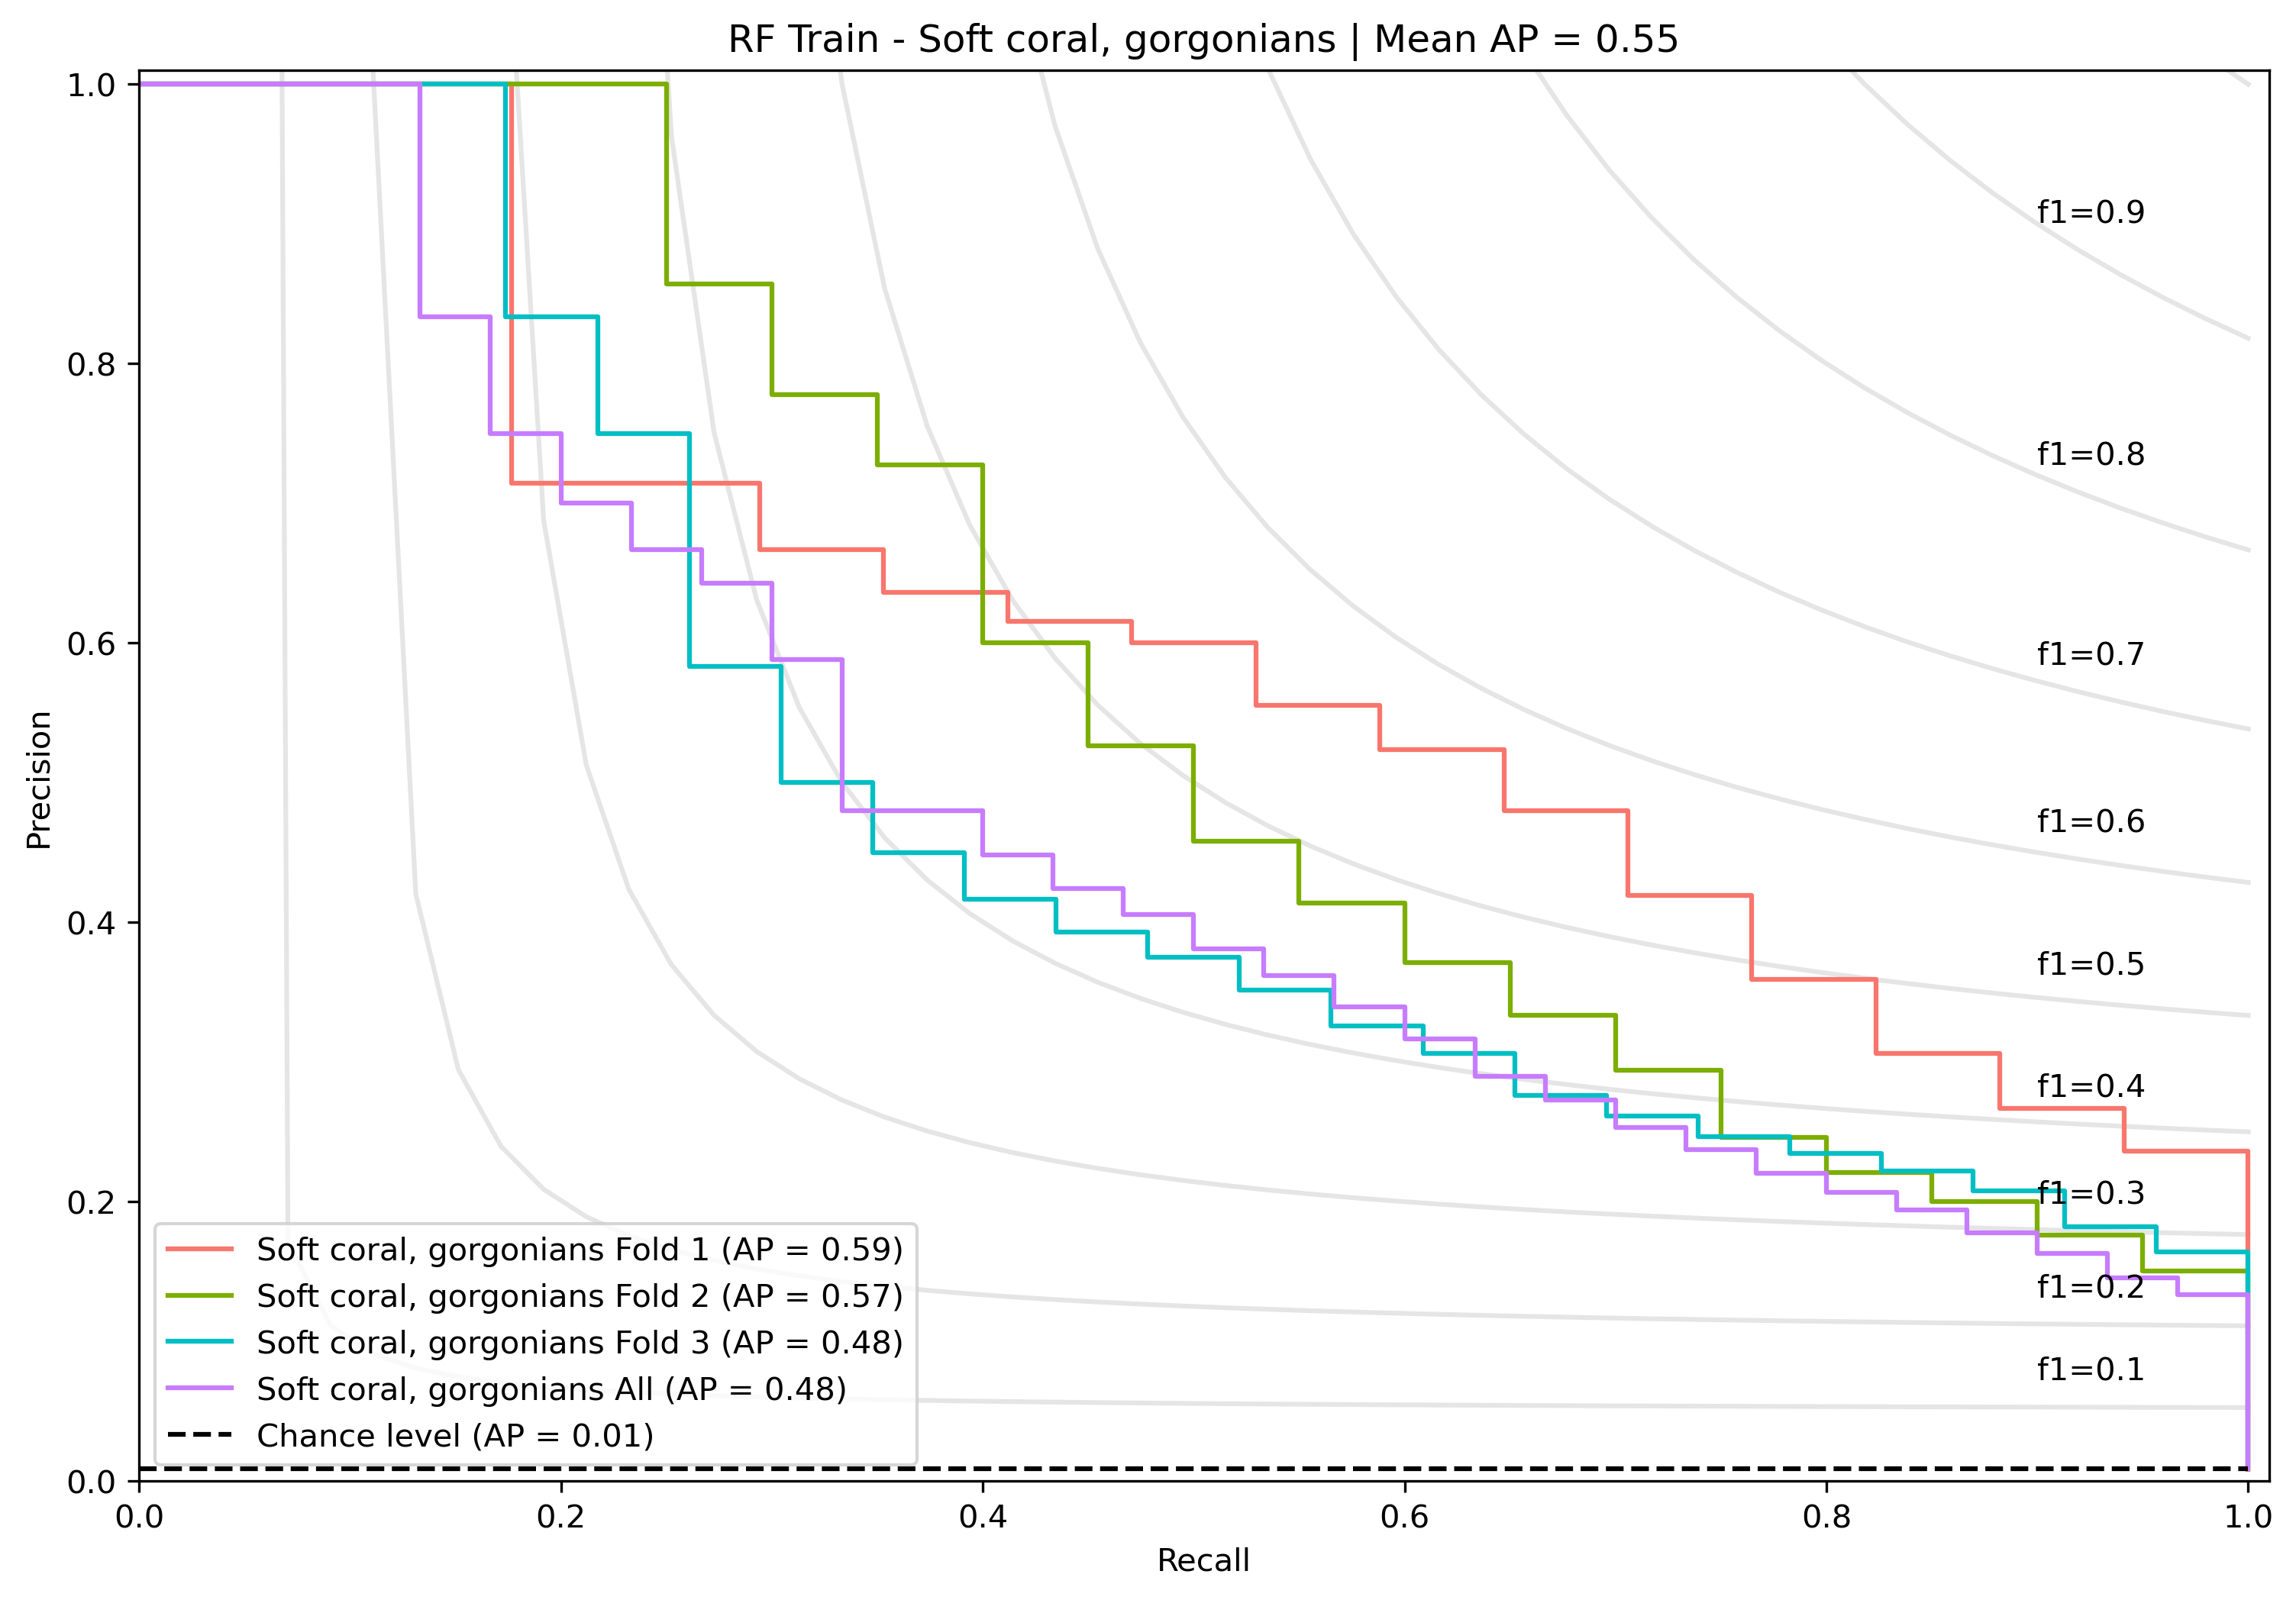
\includegraphics{03-Chapitre3/figures/supplementary/03-precision_recall_curve_train_rf_Soft coral, gorgonians.png}
\caption{AUPRC curves of the explanatory power for the Soft coral and
gorgonians. The grey lines represent isolines of
F1-score.}\label{fig:chap3figS33}
}
\end{figure}

\begin{figure}
\hypertarget{fig:chap3figS34}{%
\centering
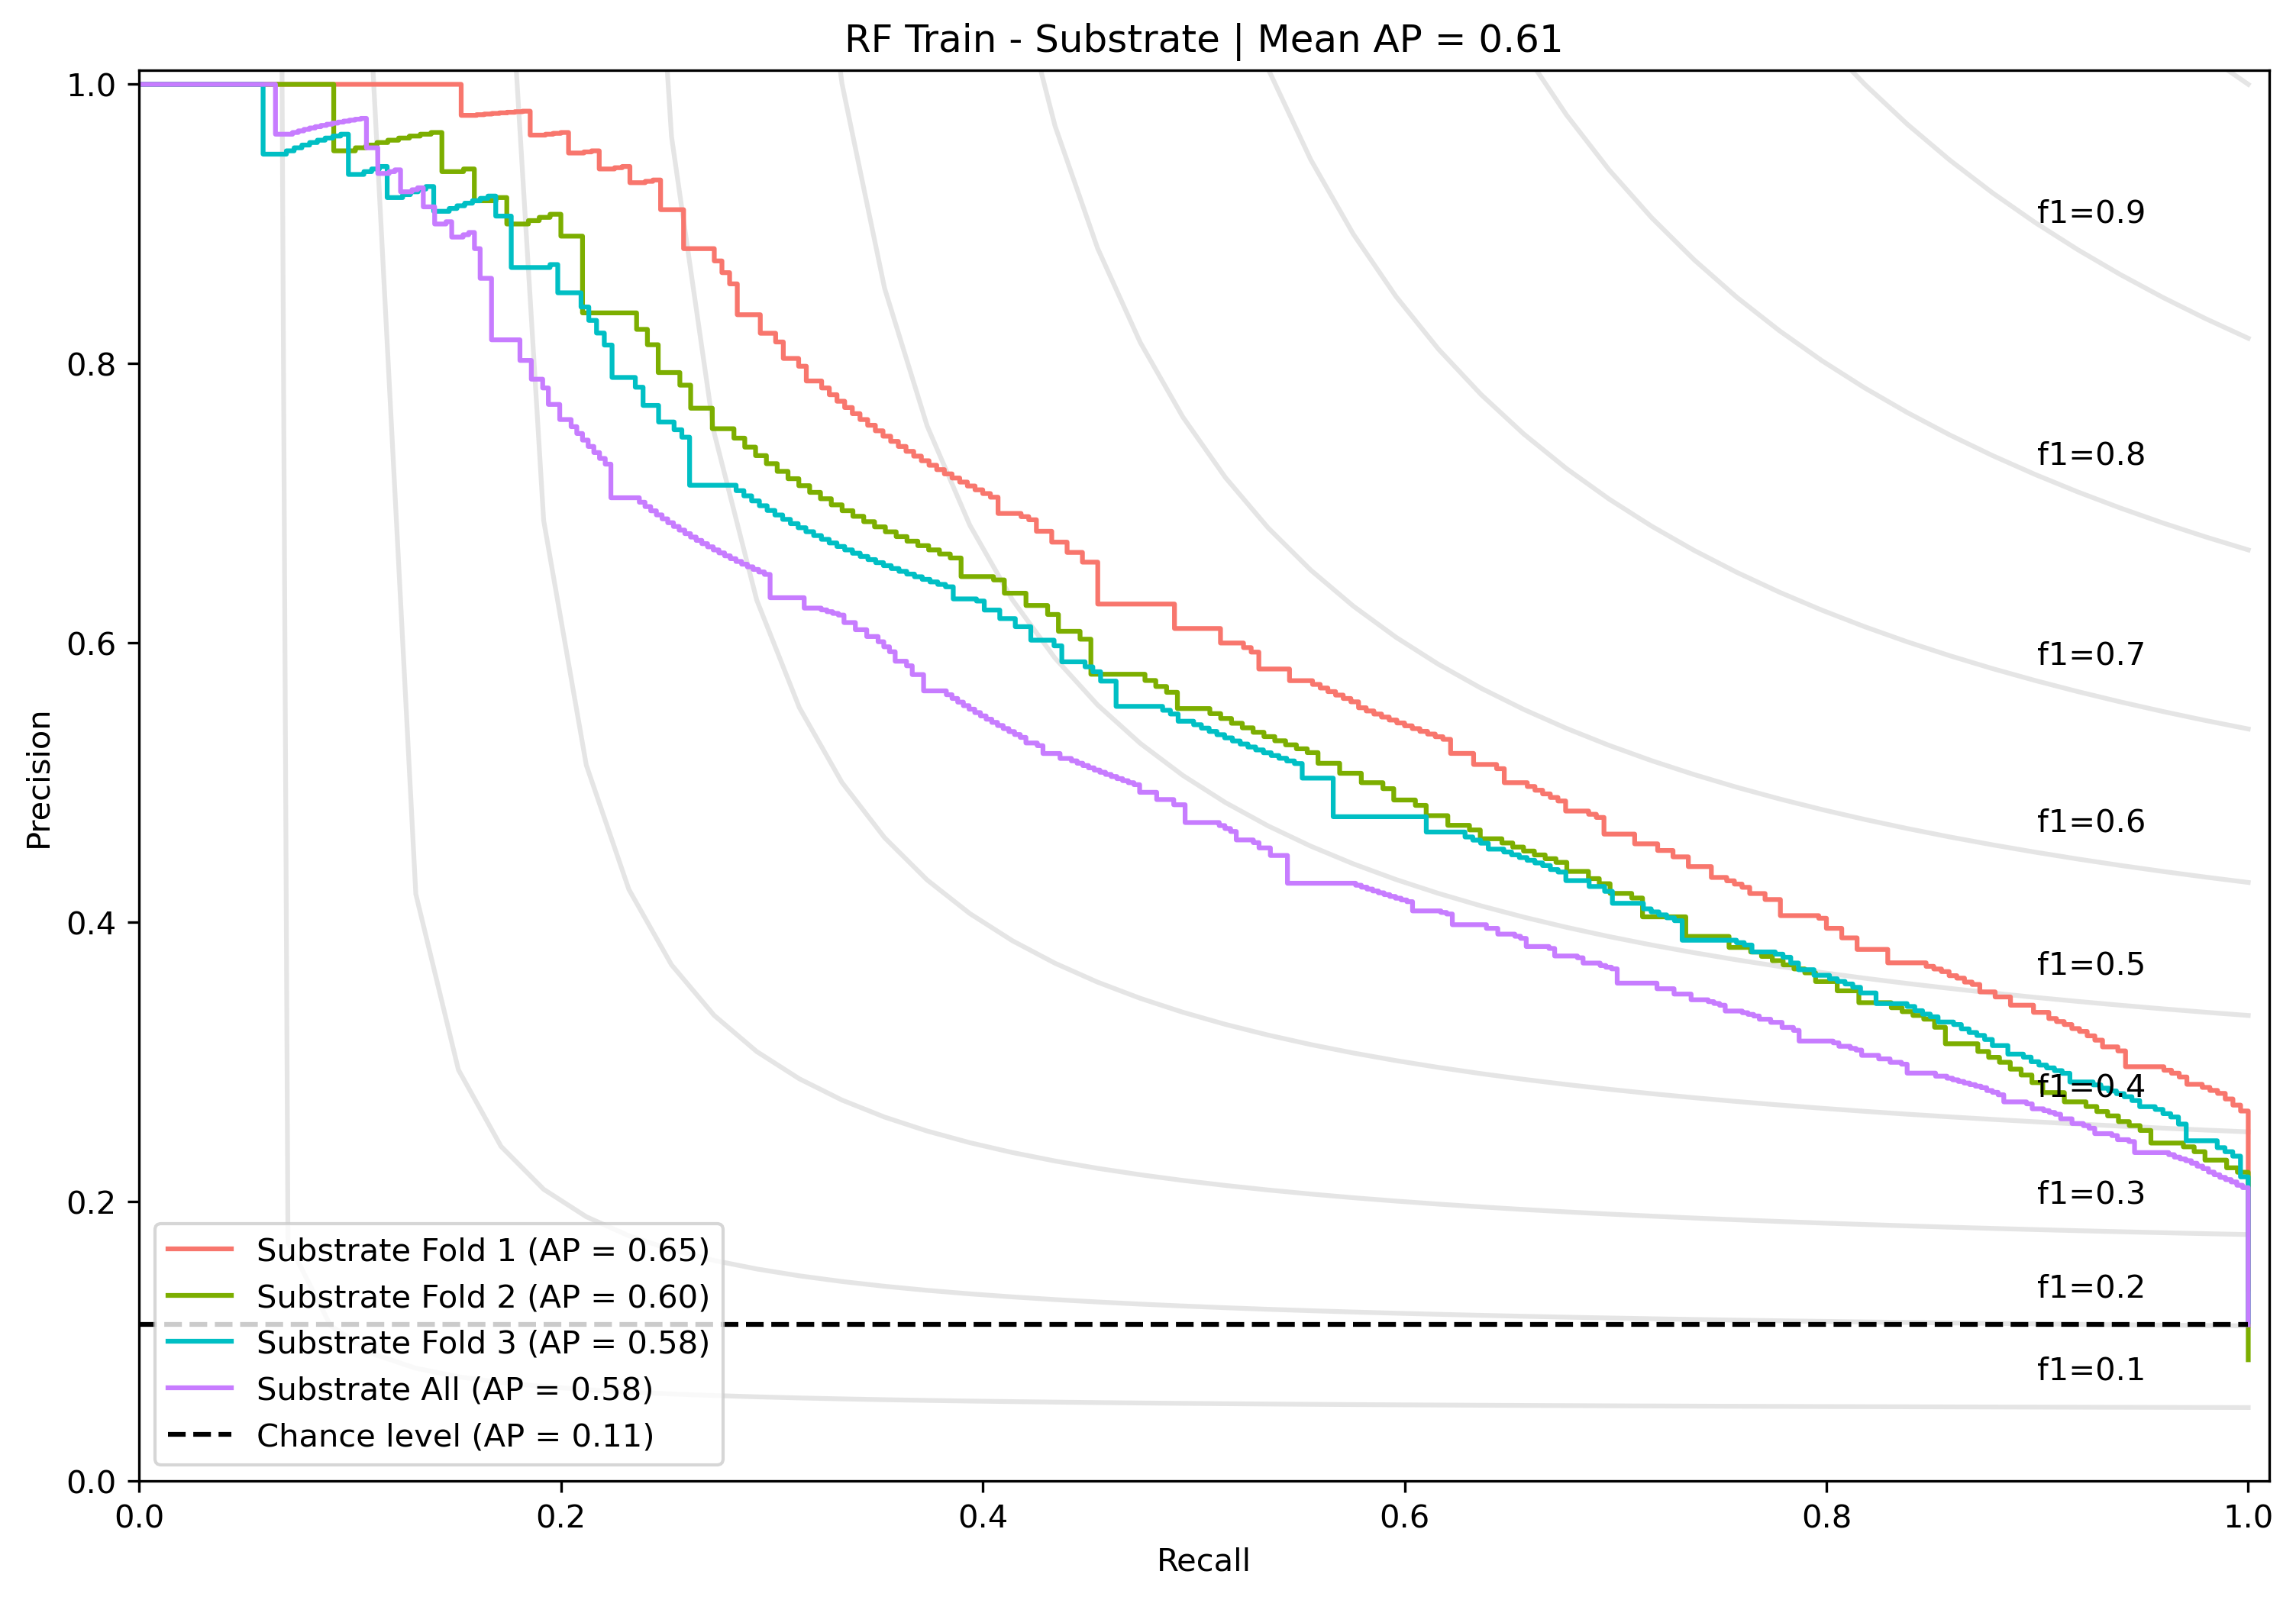
\includegraphics{03-Chapitre3/figures/supplementary/03-precision_recall_curve_train_rf_Substrate.png}
\caption{AUPRC curves of the explanatory power for the Substrate.The
grey lines represent isolines of F1-score.}\label{fig:chap3figS34}
}
\end{figure}

\begin{figure}
\hypertarget{fig:chap3figS35}{%
\centering
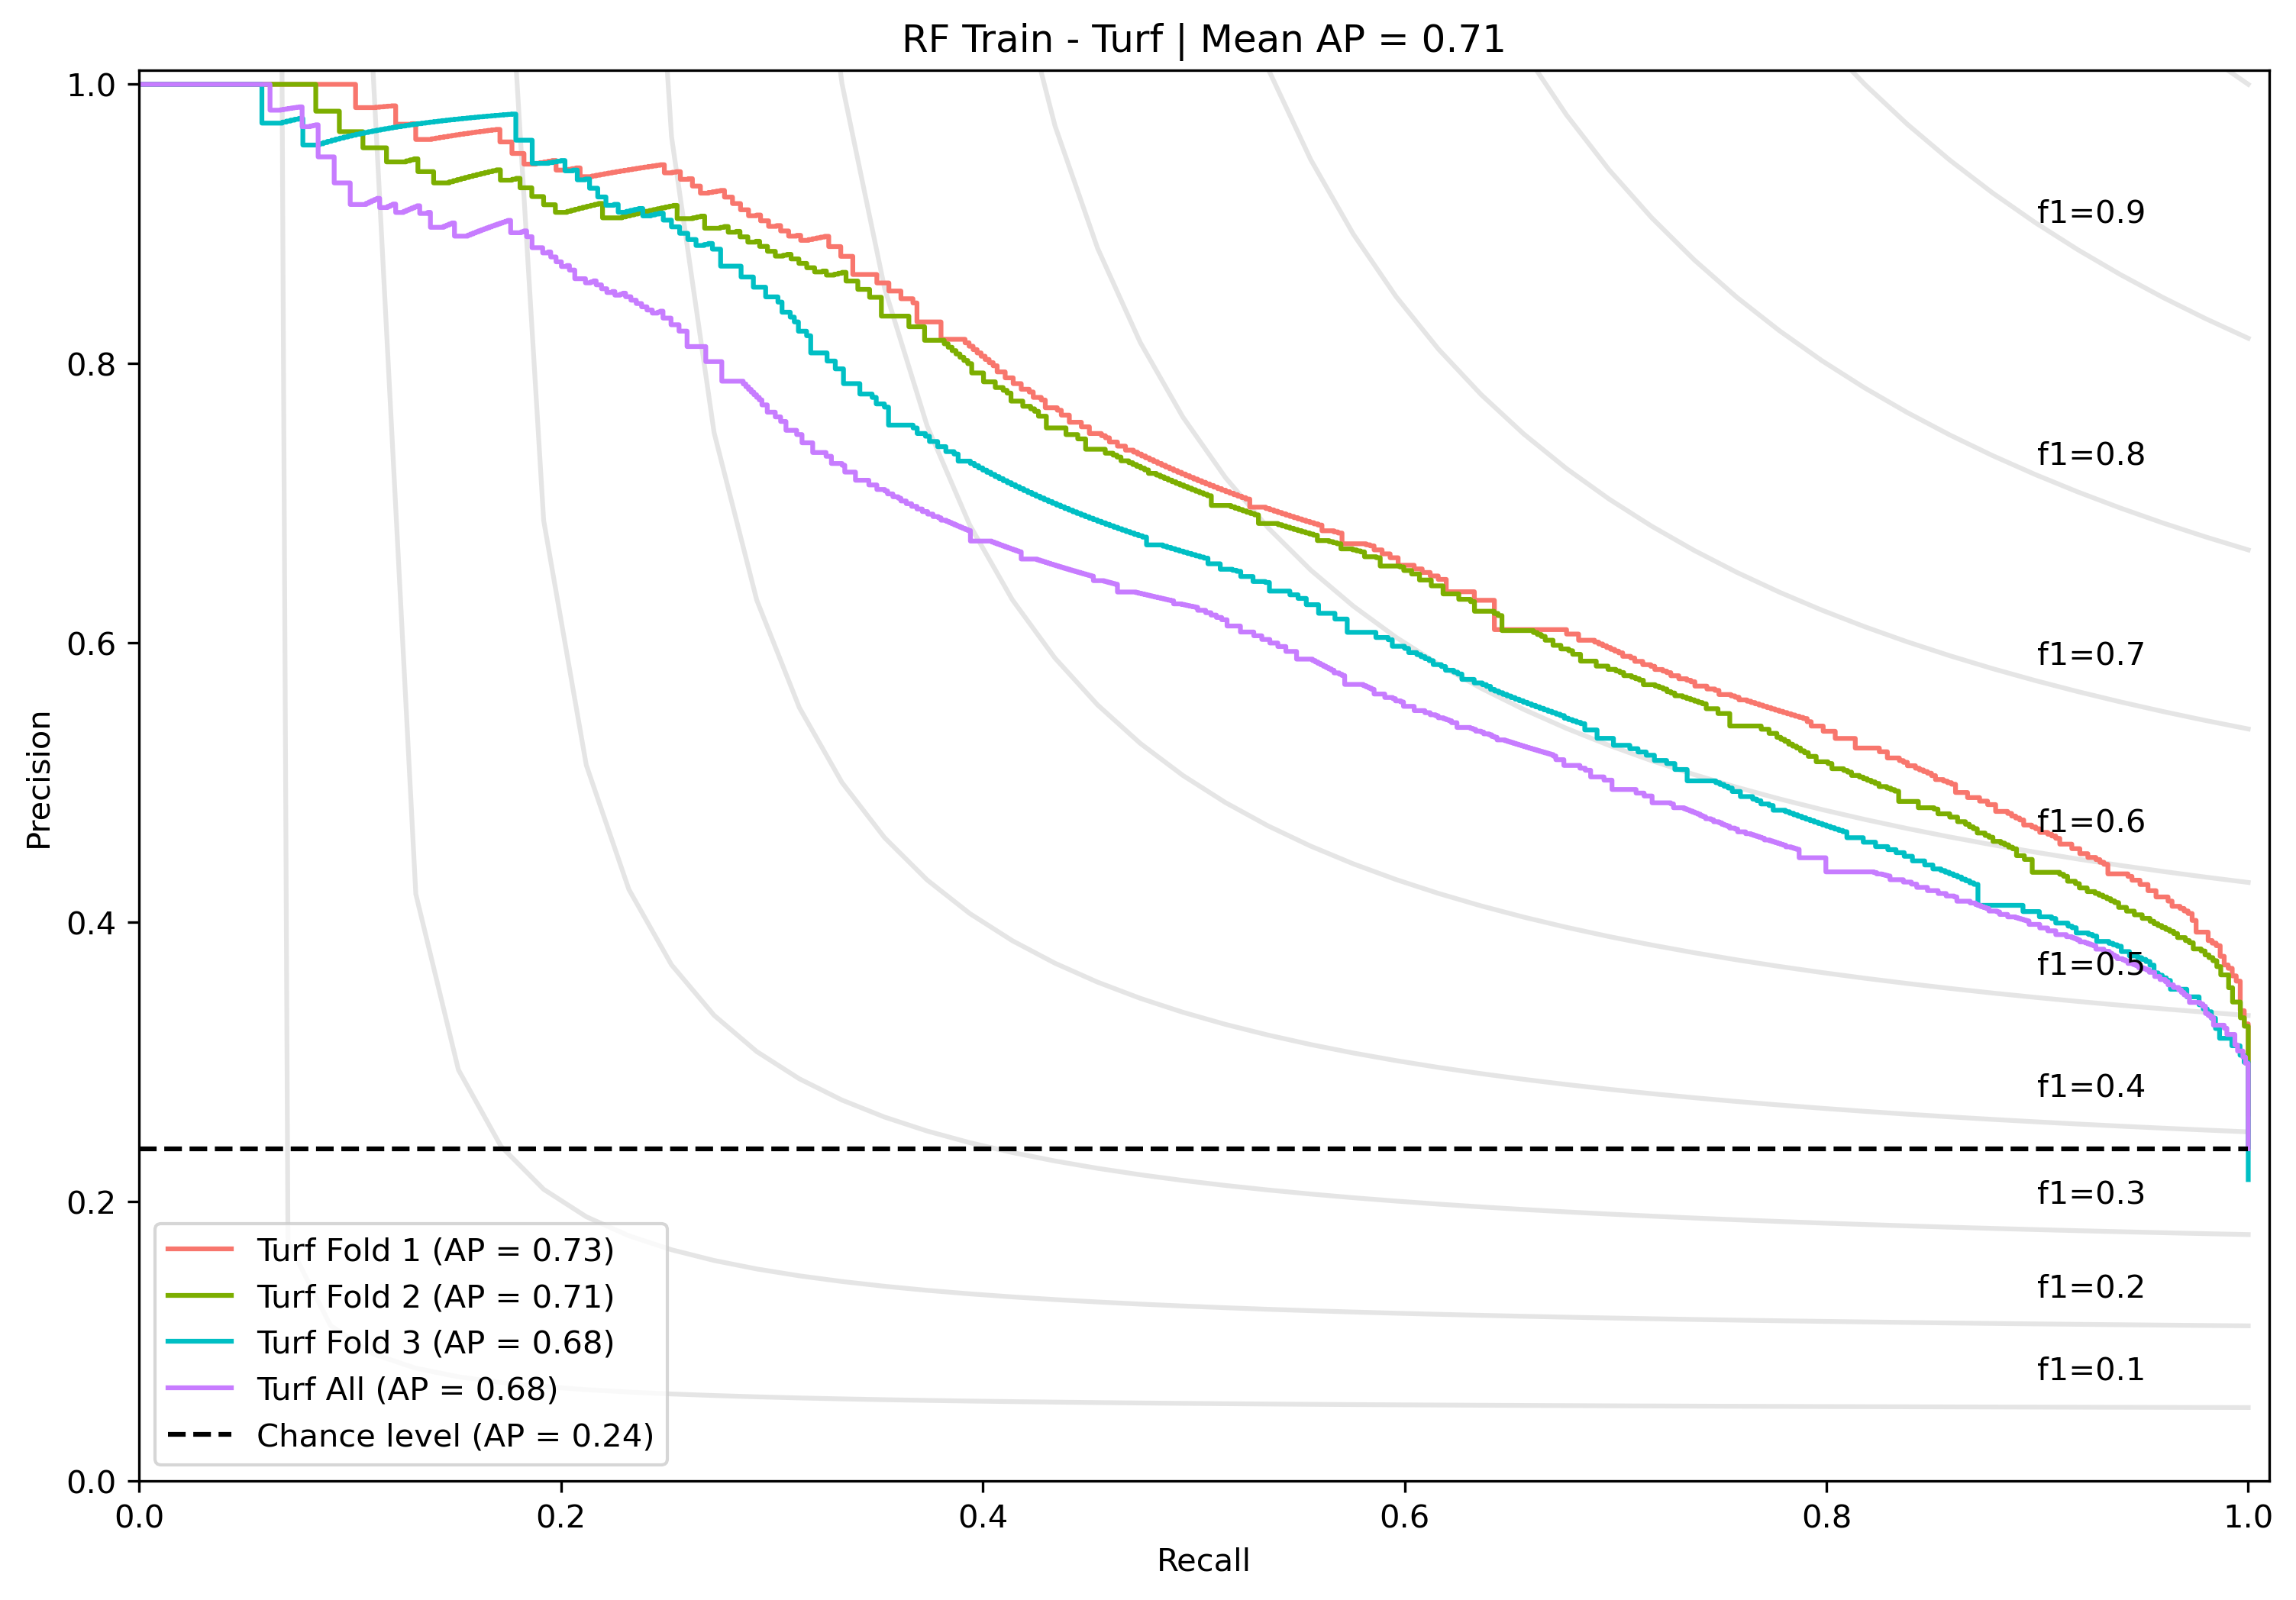
\includegraphics{03-Chapitre3/figures/supplementary/03-precision_recall_curve_train_rf_Turf.png}
\caption{AUPRC curves of the explanatory power for the Turf. The grey
lines represent isolines of F1-score.}\label{fig:chap3figS35}
}
\end{figure}

\clearpage

\hypertarget{appendixC-chapter3}{%
\section*{Appendix C - Model Explanation}\label{appendixC-chapter3}}
\addcontentsline{toc}{section}{Appendix C - Model Explanation}

\begin{figure}
\hypertarget{fig:chap3figS36}{%
\centering
\includegraphics{03-Chapitre3/figures/supplementary/04-pdp_Branching coral.png}
\caption{a. Bar plot of the three most important variables according to
the SHAP framework for Branching coral habitat state. The bars are
coloured according to the type of pressure. b. to d.~Partial Dependence
plot of these three most important variables.}\label{fig:chap3figS36}
}
\end{figure}

\begin{figure}
\hypertarget{fig:chap3figS37}{%
\centering
\includegraphics{03-Chapitre3/figures/supplementary/04-pdp_Brown algae.png}
\caption{a. Bar plot of the three most important variables according to
the SHAP framework for Brown algae habitat state. The bars are coloured
according to the type of pressure. b. to d.~Partial Dependence plot of
these three most important variables.}\label{fig:chap3figS37}
}
\end{figure}

\begin{figure}
\hypertarget{fig:chap3figS38}{%
\centering
\includegraphics{03-Chapitre3/figures/supplementary/04-pdp_Bushy Fucoid like.png}
\caption{a. Bar plot of the three most important variables according to
the SHAP framework for Bushy Fucoid like habitat state. The bars are
coloured according to the type of pressure. b. to d.~Partial Dependence
plot of these three most important variables.}\label{fig:chap3figS38}
}
\end{figure}

\begin{figure}
\hypertarget{fig:chap3figS39}{%
\centering
\includegraphics{03-Chapitre3/figures/supplementary/04-pdp_Bushy Fucoid like.png}
\caption{a. Bar plot of the three most important variables according to
the SHAP framework for Bushy Fucoid like habitat state. The bars are
coloured according to the type of pressure. b. to d.~Partial Dependence
plot of these three most important variables.}\label{fig:chap3figS39}
}
\end{figure}

\begin{figure}
\hypertarget{fig:chap3figS40}{%
\centering
\includegraphics{03-Chapitre3/figures/supplementary/04-pdp_Crustose coralline algae and turf.png}
\caption{a. Bar plot of the three most important variables according to
the SHAP framework for Crustose coralline algae and turf habitat state.
The bars are coloured according to the type of pressure. b. to
d.~Partial Dependence plot of these three most important
variables.}\label{fig:chap3figS40}
}
\end{figure}

\begin{figure}
\hypertarget{fig:chap3figS41}{%
\centering
\includegraphics{03-Chapitre3/figures/supplementary/04-pdp_Crustose coralline algae.png}
\caption{a. Bar plot of the three most important variables according to
the SHAP framework for Crustose coralline algae habitat state. The bars
are coloured according to the type of pressure. b. to d.~Partial
Dependence plot of these three most important
variables.}\label{fig:chap3figS41}
}
\end{figure}

\begin{figure}
\hypertarget{fig:chap3figS42}{%
\centering
\includegraphics{03-Chapitre3/figures/supplementary/04-pdp_Filamentous algae.png}
\caption{a. Bar plot of the three most important variables according to
the SHAP framework for Filamentous algae habitat state. The bars are
coloured according to the type of pressure. b. to d.~Partial Dependence
plot of these three most important variables.}\label{fig:chap3figS42}
}
\end{figure}

\begin{figure}
\hypertarget{fig:chap3figS43}{%
\centering
\includegraphics{03-Chapitre3/figures/supplementary/04-pdp_Green calcified algae.png}
\caption{a. Bar plot of the three most important variables according to
the SHAP framework for Green calcified algae habitat state. The bars are
coloured according to the type of pressure. b. to d.~Partial Dependence
plot of these three most important variables.}\label{fig:chap3figS43}
}
\end{figure}

\begin{figure}
\hypertarget{fig:chap3figS44}{%
\centering
\includegraphics{03-Chapitre3/figures/supplementary/04-pdp_Large canopy forming algae.png}
\caption{a. Bar plot of the three most important variables according to
the SHAP framework for Large canopy forming algae habitat state. The
bars are coloured according to the type of pressure. b. to d.~Partial
Dependence plot of these three most important
variables.}\label{fig:chap3figS44}
}
\end{figure}

\begin{figure}
\hypertarget{fig:chap3figS45}{%
\centering
\includegraphics{03-Chapitre3/figures/supplementary/04-pdp_Other Sessile invertebrates.png}
\caption{a. Bar plot of the three most important variables according to
the SHAP framework for Other Sessile invertebrates habitat state. The
bars are coloured according to the type of pressure. b. to d.~Partial
Dependence plot of these three most important
variables.}\label{fig:chap3figS45}
}
\end{figure}

\begin{figure}
\hypertarget{fig:chap3figS46}{%
\centering
\includegraphics{03-Chapitre3/figures/supplementary/04-pdp_Red algae.png}
\caption{a. Bar plot of the three most important variables according to
the SHAP framework for Red algae habitat state. The bars are coloured
according to the type of pressure. b. to d.~Partial Dependence plot of
these three most important variables.}\label{fig:chap3figS46}
}
\end{figure}

\begin{figure}
\hypertarget{fig:chap3figS47}{%
\centering
\includegraphics{03-Chapitre3/figures/supplementary/04-pdp_Seagrass.png}
\caption{a. Bar plot of the three most important variables according to
the SHAP framework for Seagrass habitat state. The bars are coloured
according to the type of pressure. b. to d.~Partial Dependence plot of
these three most important variables.}\label{fig:chap3figS47}
}
\end{figure}

\begin{figure}
\hypertarget{fig:chap3figS48}{%
\centering
\includegraphics{03-Chapitre3/figures/supplementary/04-pdp_Soft coral, gorgonians.png}
\caption{a. Bar plot of the three most important variables according to
the SHAP framework for Soft coral and gorgonians habitat state. The bars
are coloured according to the type of pressure. b. to d.~Partial
Dependence plot of these three most important
variables.}\label{fig:chap3figS48}
}
\end{figure}

\begin{figure}
\hypertarget{fig:chap3figS49}{%
\centering
\includegraphics{03-Chapitre3/figures/supplementary/04-pdp_Substrate.png}
\caption{a. Bar plot of the three most important variables according to
the SHAP framework for Substrate habitat state. The bars are coloured
according to the type of pressure. b. to d.~Partial Dependence plot of
these three most important variables.}\label{fig:chap3figS49}
}
\end{figure}

\begin{figure}
\hypertarget{fig:chap3figS50}{%
\centering
\includegraphics{03-Chapitre3/figures/supplementary/04-pdp_Turf.png}
\caption{a. Bar plot of the three most important variables according to
the SHAP framework for Turf habitat state. The bars are coloured
according to the type of pressure. b. to d.~Partial Dependence plot of
these three most important variables.}\label{fig:chap3figS50}
}
\end{figure}

% Restore all parameters as default

\let\sectionmark\oldsectionmark

\captionsetup[figure]{list=yes}
\captionsetup[table]{list=yes}

\renewcommand{\thefigure}{\arabic{figure}}
\renewcommand{\thetable}{\arabic{table}}   

% \setcounter{figure}{\value{savedfigure}}
% \setcounter{table}{\value{savedtable}}
\counterwithin{figure}{chapter}
\counterwithin{table}{chapter}

% End of subappendices environment
\AtEndEnvironment{subappendices}{%
}